% $Author$
% $Date$
% $Revision$

% HISTORY: [see also Metaprogramming2.tex]
% 2007-05-22 - Damien Pollet started (translation from French article by ...?)
% 2008-01-15 - Alex added text
% 2008-12-15 - Oscar revised
% 2009-03-24 - Stef started new chapter (acttalk ... see separate file)
% 2009-06-01 - Oscar started to revise again

%=================================================================
\ifx\wholebook\relax\else
% --------------------------------------------
% Lulu:
	\documentclass[a4paper,10pt,twoside]{book}
	\usepackage[
		papersize={6in,9in},
		hmargin={.75in,.75in},
		vmargin={.75in,1in},
		ignoreheadfoot
	]{geometry}
	% $Author$
% $Date$
% $Revision$

% HISTORY:
% 2006-10-31 - Oscar code macros
% ...

%=============================================================
% NB: documentclass must be set in main document.
% Allows book to be generated in multiple formats.
%=============================================================
%:Packages
\usepackage[T1]{fontenc}  %%%%%% really important to get the code directly in the text!
\usepackage{lmodern}
%\usepackage[scaled=0.85]{bookmanx} % needs another scale factor if used with \renewcommand{\sfdefault}{cmbr}
\usepackage{palatino}
\usepackage[scaled=0.85]{helvet}
\usepackage[protrusion,expansion=false]{microtype}
\usepackage{graphicx}
\usepackage{theorem}
\usepackage[english]{babel}
% ON: pdfsync breaks the use of p{width} for tabular columns!
\ifdefined\usepdfsync\usepackage{pdfsync}\fi % Requires texlive 2007
%=============================================================
%:More packages
%Stef should check which ones are used!
%\usepackage{picinpar}
%\usepackage{layout}
%\usepackage{color}
%\usepackage{enum}
%\usepackage{a4wide}
% \usepackage{fancyhdr}
\usepackage{ifthen}
\usepackage{float}
\usepackage{longtable}
\usepackage{makeidx}
\usepackage[nottoc]{tocbibind}
\usepackage{multicol}
\usepackage{booktabs}	% book-style tables
\usepackage{topcapt}	% enables \topcaption
\usepackage{multirow}
\usepackage{tabularx}
%\usepackage[bottom]{footmisc}
\usepackage{xspace}
\usepackage{alltt}
\usepackage{amssymb,textcomp}
\usepackage[usenames,dvipsnames]{color}
%\usepackage{colortbl}
\usepackage[hang]{subfigure}\makeatletter\def\p@subfigure{\thefigure\,}\makeatother
\usepackage{rotating}
\usepackage{enumitem}	% apb: allows more control over tags in enumerations
\usepackage{verbatim}     % for comment environment
\usepackage{varioref}	% for page references that work
\labelformat{footnote}{\thechapter--#1} % to distinguish citations from jurabib
\usepackage{needspace}
\usepackage{isodateo} % enable \isodate
\usepackage[newparttoc]{titlesec}
\usepackage{titletoc}
\usepackage{wrapfig}
\usepackage[
	super,
	citefull=first,
	authorformat={allreversed,and},
	titleformat={commasep,italic}
]{jurabib} % citations as footnotes
\usepackage[
	colorlinks=true,
	linkcolor=black,
	urlcolor=black,
	citecolor=black
]{hyperref}   % should come last
%=============================================================
%:PDF version
\pdfminorversion=3 % Set PDF to 1.3 for Lulu
%=============================================================
%:URL style
\makeatletter
\def\url@leostyle{%
  \@ifundefined{selectfont}{\def\UrlFont{\sf}}{\def\UrlFont{\sffamily}}}
\makeatother
% Now actually use the newly defined style.
\urlstyle{leo}
%=============================================================
%:Booleans
\newboolean{lulu}
\setboolean{lulu}{false}
\newcommand{\ifluluelse}[2]{\ifthenelse{\boolean{lulu}}{#1}{#2}}
%=============================================================
%:Names
\newcommand{\SUnit}{SUnit\xspace}
\newcommand{\sunit}{SUnit\xspace}
\newcommand{\xUnit}{$x$Unit\xspace}
\newcommand{\JUnit}{JUnit\xspace}
\newcommand{\st}{Smalltalk\xspace}
\newcommand{\pharo}{Pharo\xspace} % Use this, not \Pharo
%\newcommand{\sqmap}{SqueakMap\xspace}
\newcommand{\squeak}{Squeak\xspace} % use this, not \Squeak or \sq
\newcommand{\sqsrc}{SqueakSource\xspace}
\newcommand{\sbe}{\url{http://SqueakByExample.org}\xspace}
\newcommand{\pharoweb}{\url{http://pharo-project.org}\xspace}
\newcommand{\pbe}{\url{http://PharoByExample.org}\xspace}
\newcommand{\sba}{\url{http://SquareBracketAssociates.org}\xspace}
\newcommand{\bam}{\lct{Bounc\-ing\-Atoms\-Morph}\xspace}
%=============================================================
%:Markup macros for proof-reading
\usepackage[normalem]{ulem} % for \sout
\usepackage{xcolor}
\newcommand{\ra}{$\rightarrow$}
\newcommand{\ugh}[1]{\textcolor{red}{\uwave{#1}}} % please rephrase
\newcommand{\ins}[1]{\textcolor{blue}{\uline{#1}}} % please insert
\newcommand{\del}[1]{\textcolor{red}{\sout{#1}}} % please delete
\newcommand{\chg}[2]{\textcolor{red}{\sout{#1}}{\ra}\textcolor{blue}{\uline{#2}}} % please change
%=============================================================
%:Editorial comment macros
%\newcommand{\nnbb}[2]{
%    % \fbox{\bfseries\sffamily\scriptsize#1}
%    \fcolorbox{gray}{yellow}{\bfseries\sffamily\scriptsize#1}
%    {\sf\small$\blacktriangleright$\textit{#2}$\blacktriangleleft$}
%   }
\newcommand{\yellowbox}[1]{\fcolorbox{gray}{yellow}{\bfseries\sffamily\scriptsize#1}}
\newcommand{\triangles}[1]{{\sf\small$\blacktriangleright$\textit{#1}$\blacktriangleleft$}}
\newcommand{\nnbb}[2]{\yellowbox{#1} \triangles{#2}}
\newcommand{\fix}{\yellowbox{FIX!}}
\newcommand{\here}{\yellowbox{CONTINUE HERE!}}
% editor macros
\newcommand{\apl}[1]{\nnbb{Alain}{#1}} % Alain
\newcommand{\ab}[1]{\nnbb{Andrew}{#1}} % Black
\newcommand{\sd}[1]{\nnbb{St\'{e}f}{#1}} % Ducasse
\newcommand{\dc}[1]{\nnbb{DamienC}{#1}} % Ducasse
\newcommand{\md}[1]{\nnbb{Marcus}{#1}} % Denker
\newcommand{\on}[1]{\nnbb{Oscar}{#1}} % Nierstrasz
\newcommand{\damien}[1]{\nnbb{Damien}{#1}} % Pollet
\newcommand{\lr}[1]{\nnbb{Lukas}{#1}} % Renggli
\newcommand{\orla}[1]{\nnbb{Orla}{#1}} % Greevy
\newcommand{\alex}[1]{\nnbb{Alex}{#1}} % Bergel
\newcommand{\alx}[1]{\nnbb{Alex}{#1}} % Bergel
\newcommand{\dr}[1]{\nnbb{David}{#1}} % Roethlisberger
\newcommand{\ja}[1]{\nnbb{Jannik}{#1}} % Laval
\newcommand{\jr}[1]{\nnbb{Jorge}{#1}} % Ressia
\newcommand{\jb}[1]{\nnbb{JB}{#1}} % JB
\newcommand{\fp}[1]{\nnbb{Fabrizio}{#1}} % Perin
\newcommand{\michael}[1]{\nnbb{Michael}{#1}} % Davies
\newcommand{\ew}[1]{\nnbb{Erwann}{#1}} % Wernli
\newcommand{\mb}[1]{\nnbb{Martial}{#1}} % Boniou
\newcommand{\hw}[1]{\nnbb{Hernan}{#1}} % Wilkinson
\newcommand{\ben}[1]{\nnbb{Benjamin}{#1}} % Benjamin Van Ryseghem
%=============================================================
%:Abbreviation macros
\newcommand{\ie}{\emph{i.e.},\xspace}
\newcommand{\eg}{\emph{e.g.},\xspace}
\newcommand{\etc}{etc.\xspace}
%=============================================================
%:Cross reference macros
\newcommand{\charef}[1]{Chapter~\ref{cha:#1}\xspace}
\newcommand{\secref}[1]{Section~\ref{sec:#1}\xspace}
\newcommand{\figref}[1]{Figure~\ref{fig:#1}\xspace}
\newcommand{\Figref}[1]{Figure~\ref{fig:#1}\xspace}
\newcommand{\appref}[1]{Appendix~\ref{app:#1}\xspace}
\newcommand{\tabref}[1]{Table~\ref{tab:#1}\xspace}
\newcommand{\faqref}[1]{FAQ~\ref{faq:#1}, p.~\pageref{faq:#1}\xspace}
% APB: I removed trailing \xspace commands from these macros because
% \xspace mostly doesn't work.  If you want a space after your
% references, type one!
% ON: xspace has always worked just fine for me!  Please leave them in.
%
\newcommand{\ruleref}[1]{\ref{rule:#1}\xspace}
%
\newcommand{\egref}[1]{example~\ref{eg:#1}\xspace}
\newcommand{\Egref}[1]{Example~\ref{eg:#1}\xspace}
%
\newcommand{\scrref}[1]{script~\ref{scr:#1}\xspace}
\newcommand{\Scrref}[1]{Script~\ref{scr:#1}\xspace}
\newcommand{\tscrref}[1]{the script~\ref{scr:#1}\xspace}
\newcommand{\Tscrref}[1]{The script~\ref{scr:#1}\xspace}
%
\newcommand{\mthref}[1]{method~\ref{mth:#1}\xspace}
\newcommand{\mthsref}[1]{methods~\ref{mth:#1}\xspace}
\newcommand{\Mthref}[1]{Method~\ref{mth:#1}\xspace}
\newcommand{\tmthref}[1]{the method~\ref{mth:#1}\xspace}
\newcommand{\Tmthref}[1]{The method~\ref{mth:#1}\xspace}
%
\newcommand{\clsref}[1]{class~\ref{cls:#1}\xspace}
\newcommand{\tclsref}[1]{the class~\ref{cls:#1}\xspace}
\newcommand{\Tclsref}[1]{The class~\ref{cls:#1}\xspace}

\newcommand{\chalabel}[1]{\label{cha:#1}}
\newcommand{\seclabel}[1]{\label{sec:#1}}
\newcommand{\figlabel}[1]{\label{fig:#1}}
\newcommand{\tablabel}[1]{\label{tab:#1}}
\newcommand{\rulelabel}[1]{\label{rule:#1}}
\newcommand{\eglabel}[1]{\label{eg:#1}}
\newcommand{\scrlabel}[1]{\label{scr:#1}}
\newcommand{\mthlabel}[1]{\label{mth:#1}}
\newcommand{\clslabel}[1]{\label{cls:#1}}
\newcommand{\faqlabel}[1]{\label{faq:#1}}
%=============================================================
%:Menu item macro
% for menu items, so we can change our minds on how to print them! (apb)
\definecolor{lightgray}{gray}{0.89}
\newcommand{\menu}[1]{{%
	\setlength{\fboxsep}{0pt}%
	\colorbox{lightgray}{{{\upshape\sffamily\strut \,#1\,}}}}}
\newcommand{\link}[1]{{%
	\fontfamily{lmr}\selectfont
 	\upshape{\sffamily \underline{#1}}}}
% For submenu items:
\newcommand{\go}{\,$\triangleright$\,}
% \newcommand{\go}{\,$\blacktriangleright$\,}
% For keyboard shortcuts:
%\newcommand{\short}[1]{\mbox{$\langle${\sc CMD}$\rangle$-#1}\xspace}
\newcommand{\short}[1]{\mbox{{\sc cmd}\hspace{0.08em}--\hspace{0.09em}#1}\xspace}
% For buttons:
\newcommand{\button}[1]{{%
	\setlength{\fboxsep}{0pt}%
	\fbox{{\upshape\sffamily\strut \,#1\,}}}}
% NB: The button macro does not work within captions -- incompatible with xcolor package :-(
\newcommand{\toolsflap}{\textit{Tools} flap\xspace}
%=============================================================
%:Mouse clicks
\newcommand{\click}{click\xspace} % RED
\newcommand{\actclick}{action-click\xspace} % YELLOW
\newcommand{\metaclick}{meta-click\xspace} % BLUE
\newcommand{\Click}{Click\xspace} % RED
\newcommand{\Actclick}{Action-click\xspace} % YELLOW
\newcommand{\Metaclick}{Meta-click\xspace} % BLUE
%=============================================================
%:ToSh macros
\newboolean{tosh}
\setboolean{tosh}{false}
\newcommand{\iftoshelse}[2]{\ifthenelse{\boolean{tosh}}{#1}{#2}}
%=============================================================
%:ToSh colors
%\newcommand{\highlightcolor}{\color{blue!65}}
%\newcommand{\boxcolor}{\color{gray!25}}
\newcommand{\highlight}[1]{\textcolor{blue!65}{#1}}
%\newcommand{\codecolor}{\color{blue!65}}
%%\setlength{\fboxrule}{2pt}
%\newcommand{\asPict}[1]{%
%	{\Large\highlight{#1}}}
%=============================================================
%:Reader cues (do this)
%
% Indicate something the reader should try out.
% \newcommand{\dothisicon}{\raisebox{-.5ex}{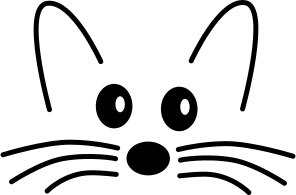
\includegraphics[width=1.4em]{squeak-logo}}}
\iftoshelse{
	\usepackage{marginnote}
		\renewcommand*{\marginfont}{\footnotesize}
	\newcommand{\vartriangleout}{\ifthenelse{\isodd{\thepage}}{\vartriangleright}{\vartriangleleft}}
	\newcommand{\dothisicon}{\fcolorbox{blue!65}{white}{\highlight{$\vartriangleout$}}}
	\newcommand{\dothis}[1]{%
		\noindent\par\noindent
		{\reversemarginpar
			\marginnote{\fcolorbox{blue!65}{white}{\highlight{$\vartriangleout$}}}}
		%\MarginLabel{do this}
		\noindent\emph{#1}
		\nopagebreak}
}{
	\newcommand{\dothisicon}{\raisebox{-.5ex}{
\includegraphics[height=1.2em]{pharo}}}
	\newcommand{\dothis}[1]{%
		\medskip
		\noindent\dothisicon
		\ifx#1\empty\else\quad\emph{#1}\fi
		\par\smallskip\nopagebreak}
}
%===> NEW VERSION <===
% NB: To use this in an individual chapter, you must set:
%\graphicspath{{figures/} {../figures/}}
% at the head of the chapter.  Don't forget the final /
%=============================================================
%:Reader hints (hint)
%
% Indicates a non-obvious consequence 
\newcommand{\hint}[1]{\vspace{1ex}\noindent\fbox{\textsc{Hint}} \emph{#1}}
%=================================================================
% graphics for Morphic handles
\newcommand{\grabHandle}{\raisebox{-0.2ex}{
\includegraphics[width=1em]{blackHandle}}}
\newcommand{\moveHandle}{\raisebox{-0.2ex}{
\includegraphics[width=1em]{moveHandle}}}
\newcommand{\debugHandle}{\raisebox{-0.2ex}{
\includegraphics[width=1em]{debugHandle}}}
%=============================================================
%:Highlighting Important stuff (doublebox)
%
% From Seaside book ...
\newsavebox{\SavedText}
\newlength{\InnerBoxRule}\setlength{\InnerBoxRule}{.75\fboxrule}
\newlength{\OuterBoxRule}\setlength{\OuterBoxRule}{1.5\fboxrule}
\newlength{\BoxSeparation}\setlength{\BoxSeparation}{1.5\fboxrule}
\addtolength{\BoxSeparation}{.5pt}
\newlength{\SaveBoxSep}\setlength{\SaveBoxSep}{2\fboxsep}
%
\newenvironment{doublebox}{\begin{lrbox}{\SavedText}
    \begin{minipage}{.75\textwidth}}
    {\end{minipage}\end{lrbox}\begin{center}
    \setlength{\fboxsep}{\BoxSeparation}\setlength{\fboxrule}{\OuterBoxRule}
    \fbox{\setlength{\fboxsep}{\SaveBoxSep}\setlength{\fboxrule}{\InnerBoxRule}%
      \fbox{\usebox{\SavedText}}}
  \end{center}}
% Use this:
\newcommand{\important}[1]{\begin{doublebox}#1\end{doublebox}}
%=============================================================
%:Section depth
\setcounter{secnumdepth}{2}
%% for this to happen start the file with
%\ifx\wholebook\relax\else
%% $Author$
% $Date$
% $Revision$

% HISTORY:
% 2006-10-31 - Oscar code macros
% ...

%=============================================================
% NB: documentclass must be set in main document.
% Allows book to be generated in multiple formats.
%=============================================================
%:Packages
\usepackage[T1]{fontenc}  %%%%%% really important to get the code directly in the text!
\usepackage{lmodern}
%\usepackage[scaled=0.85]{bookmanx} % needs another scale factor if used with \renewcommand{\sfdefault}{cmbr}
\usepackage{palatino}
\usepackage[scaled=0.85]{helvet}
\usepackage[protrusion,expansion=false]{microtype}
\usepackage{graphicx}
\usepackage{theorem}
\usepackage[english]{babel}
% ON: pdfsync breaks the use of p{width} for tabular columns!
\ifdefined\usepdfsync\usepackage{pdfsync}\fi % Requires texlive 2007
%=============================================================
%:More packages
%Stef should check which ones are used!
%\usepackage{picinpar}
%\usepackage{layout}
%\usepackage{color}
%\usepackage{enum}
%\usepackage{a4wide}
% \usepackage{fancyhdr}
\usepackage{ifthen}
\usepackage{float}
\usepackage{longtable}
\usepackage{makeidx}
\usepackage[nottoc]{tocbibind}
\usepackage{multicol}
\usepackage{booktabs}	% book-style tables
\usepackage{topcapt}	% enables \topcaption
\usepackage{multirow}
\usepackage{tabularx}
%\usepackage[bottom]{footmisc}
\usepackage{xspace}
\usepackage{alltt}
\usepackage{amssymb,textcomp}
\usepackage[usenames,dvipsnames]{color}
%\usepackage{colortbl}
\usepackage[hang]{subfigure}\makeatletter\def\p@subfigure{\thefigure\,}\makeatother
\usepackage{rotating}
\usepackage{enumitem}	% apb: allows more control over tags in enumerations
\usepackage{verbatim}     % for comment environment
\usepackage{varioref}	% for page references that work
\labelformat{footnote}{\thechapter--#1} % to distinguish citations from jurabib
\usepackage{needspace}
\usepackage{isodateo} % enable \isodate
\usepackage[newparttoc]{titlesec}
\usepackage{titletoc}
\usepackage{wrapfig}
\usepackage[
	super,
	citefull=first,
	authorformat={allreversed,and},
	titleformat={commasep,italic}
]{jurabib} % citations as footnotes
\usepackage[
	colorlinks=true,
	linkcolor=black,
	urlcolor=black,
	citecolor=black
]{hyperref}   % should come last
%=============================================================
%:PDF version
\pdfminorversion=3 % Set PDF to 1.3 for Lulu
%=============================================================
%:URL style
\makeatletter
\def\url@leostyle{%
  \@ifundefined{selectfont}{\def\UrlFont{\sf}}{\def\UrlFont{\sffamily}}}
\makeatother
% Now actually use the newly defined style.
\urlstyle{leo}
%=============================================================
%:Booleans
\newboolean{lulu}
\setboolean{lulu}{false}
\newcommand{\ifluluelse}[2]{\ifthenelse{\boolean{lulu}}{#1}{#2}}
%=============================================================
%:Names
\newcommand{\SUnit}{SUnit\xspace}
\newcommand{\sunit}{SUnit\xspace}
\newcommand{\xUnit}{$x$Unit\xspace}
\newcommand{\JUnit}{JUnit\xspace}
\newcommand{\st}{Smalltalk\xspace}
\newcommand{\pharo}{Pharo\xspace} % Use this, not \Pharo
%\newcommand{\sqmap}{SqueakMap\xspace}
\newcommand{\squeak}{Squeak\xspace} % use this, not \Squeak or \sq
\newcommand{\sqsrc}{SqueakSource\xspace}
\newcommand{\sbe}{\url{http://SqueakByExample.org}\xspace}
\newcommand{\pharoweb}{\url{http://pharo-project.org}\xspace}
\newcommand{\pbe}{\url{http://PharoByExample.org}\xspace}
\newcommand{\sba}{\url{http://SquareBracketAssociates.org}\xspace}
\newcommand{\bam}{\lct{Bounc\-ing\-Atoms\-Morph}\xspace}
%=============================================================
%:Markup macros for proof-reading
\usepackage[normalem]{ulem} % for \sout
\usepackage{xcolor}
\newcommand{\ra}{$\rightarrow$}
\newcommand{\ugh}[1]{\textcolor{red}{\uwave{#1}}} % please rephrase
\newcommand{\ins}[1]{\textcolor{blue}{\uline{#1}}} % please insert
\newcommand{\del}[1]{\textcolor{red}{\sout{#1}}} % please delete
\newcommand{\chg}[2]{\textcolor{red}{\sout{#1}}{\ra}\textcolor{blue}{\uline{#2}}} % please change
%=============================================================
%:Editorial comment macros
%\newcommand{\nnbb}[2]{
%    % \fbox{\bfseries\sffamily\scriptsize#1}
%    \fcolorbox{gray}{yellow}{\bfseries\sffamily\scriptsize#1}
%    {\sf\small$\blacktriangleright$\textit{#2}$\blacktriangleleft$}
%   }
\newcommand{\yellowbox}[1]{\fcolorbox{gray}{yellow}{\bfseries\sffamily\scriptsize#1}}
\newcommand{\triangles}[1]{{\sf\small$\blacktriangleright$\textit{#1}$\blacktriangleleft$}}
\newcommand{\nnbb}[2]{\yellowbox{#1} \triangles{#2}}
\newcommand{\fix}{\yellowbox{FIX!}}
\newcommand{\here}{\yellowbox{CONTINUE HERE!}}
% editor macros
\newcommand{\apl}[1]{\nnbb{Alain}{#1}} % Alain
\newcommand{\ab}[1]{\nnbb{Andrew}{#1}} % Black
\newcommand{\sd}[1]{\nnbb{St\'{e}f}{#1}} % Ducasse
\newcommand{\dc}[1]{\nnbb{DamienC}{#1}} % Ducasse
\newcommand{\md}[1]{\nnbb{Marcus}{#1}} % Denker
\newcommand{\on}[1]{\nnbb{Oscar}{#1}} % Nierstrasz
\newcommand{\damien}[1]{\nnbb{Damien}{#1}} % Pollet
\newcommand{\lr}[1]{\nnbb{Lukas}{#1}} % Renggli
\newcommand{\orla}[1]{\nnbb{Orla}{#1}} % Greevy
\newcommand{\alex}[1]{\nnbb{Alex}{#1}} % Bergel
\newcommand{\alx}[1]{\nnbb{Alex}{#1}} % Bergel
\newcommand{\dr}[1]{\nnbb{David}{#1}} % Roethlisberger
\newcommand{\ja}[1]{\nnbb{Jannik}{#1}} % Laval
\newcommand{\jr}[1]{\nnbb{Jorge}{#1}} % Ressia
\newcommand{\jb}[1]{\nnbb{JB}{#1}} % JB
\newcommand{\fp}[1]{\nnbb{Fabrizio}{#1}} % Perin
\newcommand{\michael}[1]{\nnbb{Michael}{#1}} % Davies
\newcommand{\ew}[1]{\nnbb{Erwann}{#1}} % Wernli
\newcommand{\mb}[1]{\nnbb{Martial}{#1}} % Boniou
\newcommand{\hw}[1]{\nnbb{Hernan}{#1}} % Wilkinson
\newcommand{\ben}[1]{\nnbb{Benjamin}{#1}} % Benjamin Van Ryseghem
%=============================================================
%:Abbreviation macros
\newcommand{\ie}{\emph{i.e.},\xspace}
\newcommand{\eg}{\emph{e.g.},\xspace}
\newcommand{\etc}{etc.\xspace}
%=============================================================
%:Cross reference macros
\newcommand{\charef}[1]{Chapter~\ref{cha:#1}\xspace}
\newcommand{\secref}[1]{Section~\ref{sec:#1}\xspace}
\newcommand{\figref}[1]{Figure~\ref{fig:#1}\xspace}
\newcommand{\Figref}[1]{Figure~\ref{fig:#1}\xspace}
\newcommand{\appref}[1]{Appendix~\ref{app:#1}\xspace}
\newcommand{\tabref}[1]{Table~\ref{tab:#1}\xspace}
\newcommand{\faqref}[1]{FAQ~\ref{faq:#1}, p.~\pageref{faq:#1}\xspace}
% APB: I removed trailing \xspace commands from these macros because
% \xspace mostly doesn't work.  If you want a space after your
% references, type one!
% ON: xspace has always worked just fine for me!  Please leave them in.
%
\newcommand{\ruleref}[1]{\ref{rule:#1}\xspace}
%
\newcommand{\egref}[1]{example~\ref{eg:#1}\xspace}
\newcommand{\Egref}[1]{Example~\ref{eg:#1}\xspace}
%
\newcommand{\scrref}[1]{script~\ref{scr:#1}\xspace}
\newcommand{\Scrref}[1]{Script~\ref{scr:#1}\xspace}
\newcommand{\tscrref}[1]{the script~\ref{scr:#1}\xspace}
\newcommand{\Tscrref}[1]{The script~\ref{scr:#1}\xspace}
%
\newcommand{\mthref}[1]{method~\ref{mth:#1}\xspace}
\newcommand{\mthsref}[1]{methods~\ref{mth:#1}\xspace}
\newcommand{\Mthref}[1]{Method~\ref{mth:#1}\xspace}
\newcommand{\tmthref}[1]{the method~\ref{mth:#1}\xspace}
\newcommand{\Tmthref}[1]{The method~\ref{mth:#1}\xspace}
%
\newcommand{\clsref}[1]{class~\ref{cls:#1}\xspace}
\newcommand{\tclsref}[1]{the class~\ref{cls:#1}\xspace}
\newcommand{\Tclsref}[1]{The class~\ref{cls:#1}\xspace}

\newcommand{\chalabel}[1]{\label{cha:#1}}
\newcommand{\seclabel}[1]{\label{sec:#1}}
\newcommand{\figlabel}[1]{\label{fig:#1}}
\newcommand{\tablabel}[1]{\label{tab:#1}}
\newcommand{\rulelabel}[1]{\label{rule:#1}}
\newcommand{\eglabel}[1]{\label{eg:#1}}
\newcommand{\scrlabel}[1]{\label{scr:#1}}
\newcommand{\mthlabel}[1]{\label{mth:#1}}
\newcommand{\clslabel}[1]{\label{cls:#1}}
\newcommand{\faqlabel}[1]{\label{faq:#1}}
%=============================================================
%:Menu item macro
% for menu items, so we can change our minds on how to print them! (apb)
\definecolor{lightgray}{gray}{0.89}
\newcommand{\menu}[1]{{%
	\setlength{\fboxsep}{0pt}%
	\colorbox{lightgray}{{{\upshape\sffamily\strut \,#1\,}}}}}
\newcommand{\link}[1]{{%
	\fontfamily{lmr}\selectfont
 	\upshape{\sffamily \underline{#1}}}}
% For submenu items:
\newcommand{\go}{\,$\triangleright$\,}
% \newcommand{\go}{\,$\blacktriangleright$\,}
% For keyboard shortcuts:
%\newcommand{\short}[1]{\mbox{$\langle${\sc CMD}$\rangle$-#1}\xspace}
\newcommand{\short}[1]{\mbox{{\sc cmd}\hspace{0.08em}--\hspace{0.09em}#1}\xspace}
% For buttons:
\newcommand{\button}[1]{{%
	\setlength{\fboxsep}{0pt}%
	\fbox{{\upshape\sffamily\strut \,#1\,}}}}
% NB: The button macro does not work within captions -- incompatible with xcolor package :-(
\newcommand{\toolsflap}{\textit{Tools} flap\xspace}
%=============================================================
%:Mouse clicks
\newcommand{\click}{click\xspace} % RED
\newcommand{\actclick}{action-click\xspace} % YELLOW
\newcommand{\metaclick}{meta-click\xspace} % BLUE
\newcommand{\Click}{Click\xspace} % RED
\newcommand{\Actclick}{Action-click\xspace} % YELLOW
\newcommand{\Metaclick}{Meta-click\xspace} % BLUE
%=============================================================
%:ToSh macros
\newboolean{tosh}
\setboolean{tosh}{false}
\newcommand{\iftoshelse}[2]{\ifthenelse{\boolean{tosh}}{#1}{#2}}
%=============================================================
%:ToSh colors
%\newcommand{\highlightcolor}{\color{blue!65}}
%\newcommand{\boxcolor}{\color{gray!25}}
\newcommand{\highlight}[1]{\textcolor{blue!65}{#1}}
%\newcommand{\codecolor}{\color{blue!65}}
%%\setlength{\fboxrule}{2pt}
%\newcommand{\asPict}[1]{%
%	{\Large\highlight{#1}}}
%=============================================================
%:Reader cues (do this)
%
% Indicate something the reader should try out.
% \newcommand{\dothisicon}{\raisebox{-.5ex}{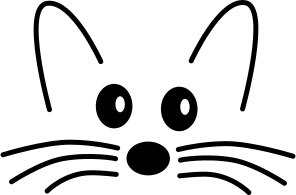
\includegraphics[width=1.4em]{squeak-logo}}}
\iftoshelse{
	\usepackage{marginnote}
		\renewcommand*{\marginfont}{\footnotesize}
	\newcommand{\vartriangleout}{\ifthenelse{\isodd{\thepage}}{\vartriangleright}{\vartriangleleft}}
	\newcommand{\dothisicon}{\fcolorbox{blue!65}{white}{\highlight{$\vartriangleout$}}}
	\newcommand{\dothis}[1]{%
		\noindent\par\noindent
		{\reversemarginpar
			\marginnote{\fcolorbox{blue!65}{white}{\highlight{$\vartriangleout$}}}}
		%\MarginLabel{do this}
		\noindent\emph{#1}
		\nopagebreak}
}{
	\newcommand{\dothisicon}{\raisebox{-.5ex}{
\includegraphics[height=1.2em]{pharo}}}
	\newcommand{\dothis}[1]{%
		\medskip
		\noindent\dothisicon
		\ifx#1\empty\else\quad\emph{#1}\fi
		\par\smallskip\nopagebreak}
}
%===> NEW VERSION <===
% NB: To use this in an individual chapter, you must set:
%\graphicspath{{figures/} {../figures/}}
% at the head of the chapter.  Don't forget the final /
%=============================================================
%:Reader hints (hint)
%
% Indicates a non-obvious consequence 
\newcommand{\hint}[1]{\vspace{1ex}\noindent\fbox{\textsc{Hint}} \emph{#1}}
%=================================================================
% graphics for Morphic handles
\newcommand{\grabHandle}{\raisebox{-0.2ex}{
\includegraphics[width=1em]{blackHandle}}}
\newcommand{\moveHandle}{\raisebox{-0.2ex}{
\includegraphics[width=1em]{moveHandle}}}
\newcommand{\debugHandle}{\raisebox{-0.2ex}{
\includegraphics[width=1em]{debugHandle}}}
%=============================================================
%:Highlighting Important stuff (doublebox)
%
% From Seaside book ...
\newsavebox{\SavedText}
\newlength{\InnerBoxRule}\setlength{\InnerBoxRule}{.75\fboxrule}
\newlength{\OuterBoxRule}\setlength{\OuterBoxRule}{1.5\fboxrule}
\newlength{\BoxSeparation}\setlength{\BoxSeparation}{1.5\fboxrule}
\addtolength{\BoxSeparation}{.5pt}
\newlength{\SaveBoxSep}\setlength{\SaveBoxSep}{2\fboxsep}
%
\newenvironment{doublebox}{\begin{lrbox}{\SavedText}
    \begin{minipage}{.75\textwidth}}
    {\end{minipage}\end{lrbox}\begin{center}
    \setlength{\fboxsep}{\BoxSeparation}\setlength{\fboxrule}{\OuterBoxRule}
    \fbox{\setlength{\fboxsep}{\SaveBoxSep}\setlength{\fboxrule}{\InnerBoxRule}%
      \fbox{\usebox{\SavedText}}}
  \end{center}}
% Use this:
\newcommand{\important}[1]{\begin{doublebox}#1\end{doublebox}}
%=============================================================
%:Section depth
\setcounter{secnumdepth}{2}
%% for this to happen start the file with
%\ifx\wholebook\relax\else
%% $Author$
% $Date$
% $Revision$

% HISTORY:
% 2006-10-31 - Oscar code macros
% ...

%=============================================================
% NB: documentclass must be set in main document.
% Allows book to be generated in multiple formats.
%=============================================================
%:Packages
\usepackage[T1]{fontenc}  %%%%%% really important to get the code directly in the text!
\usepackage{lmodern}
%\usepackage[scaled=0.85]{bookmanx} % needs another scale factor if used with \renewcommand{\sfdefault}{cmbr}
\usepackage{palatino}
\usepackage[scaled=0.85]{helvet}
\usepackage[protrusion,expansion=false]{microtype}
\usepackage{graphicx}
\usepackage{theorem}
\usepackage[english]{babel}
% ON: pdfsync breaks the use of p{width} for tabular columns!
\ifdefined\usepdfsync\usepackage{pdfsync}\fi % Requires texlive 2007
%=============================================================
%:More packages
%Stef should check which ones are used!
%\usepackage{picinpar}
%\usepackage{layout}
%\usepackage{color}
%\usepackage{enum}
%\usepackage{a4wide}
% \usepackage{fancyhdr}
\usepackage{ifthen}
\usepackage{float}
\usepackage{longtable}
\usepackage{makeidx}
\usepackage[nottoc]{tocbibind}
\usepackage{multicol}
\usepackage{booktabs}	% book-style tables
\usepackage{topcapt}	% enables \topcaption
\usepackage{multirow}
\usepackage{tabularx}
%\usepackage[bottom]{footmisc}
\usepackage{xspace}
\usepackage{alltt}
\usepackage{amssymb,textcomp}
\usepackage[usenames,dvipsnames]{color}
%\usepackage{colortbl}
\usepackage[hang]{subfigure}\makeatletter\def\p@subfigure{\thefigure\,}\makeatother
\usepackage{rotating}
\usepackage{enumitem}	% apb: allows more control over tags in enumerations
\usepackage{verbatim}     % for comment environment
\usepackage{varioref}	% for page references that work
\labelformat{footnote}{\thechapter--#1} % to distinguish citations from jurabib
\usepackage{needspace}
\usepackage{isodateo} % enable \isodate
\usepackage[newparttoc]{titlesec}
\usepackage{titletoc}
\usepackage{wrapfig}
\usepackage[
	super,
	citefull=first,
	authorformat={allreversed,and},
	titleformat={commasep,italic}
]{jurabib} % citations as footnotes
\usepackage[
	colorlinks=true,
	linkcolor=black,
	urlcolor=black,
	citecolor=black
]{hyperref}   % should come last
%=============================================================
%:PDF version
\pdfminorversion=3 % Set PDF to 1.3 for Lulu
%=============================================================
%:URL style
\makeatletter
\def\url@leostyle{%
  \@ifundefined{selectfont}{\def\UrlFont{\sf}}{\def\UrlFont{\sffamily}}}
\makeatother
% Now actually use the newly defined style.
\urlstyle{leo}
%=============================================================
%:Booleans
\newboolean{lulu}
\setboolean{lulu}{false}
\newcommand{\ifluluelse}[2]{\ifthenelse{\boolean{lulu}}{#1}{#2}}
%=============================================================
%:Names
\newcommand{\SUnit}{SUnit\xspace}
\newcommand{\sunit}{SUnit\xspace}
\newcommand{\xUnit}{$x$Unit\xspace}
\newcommand{\JUnit}{JUnit\xspace}
\newcommand{\st}{Smalltalk\xspace}
\newcommand{\pharo}{Pharo\xspace} % Use this, not \Pharo
%\newcommand{\sqmap}{SqueakMap\xspace}
\newcommand{\squeak}{Squeak\xspace} % use this, not \Squeak or \sq
\newcommand{\sqsrc}{SqueakSource\xspace}
\newcommand{\sbe}{\url{http://SqueakByExample.org}\xspace}
\newcommand{\pharoweb}{\url{http://pharo-project.org}\xspace}
\newcommand{\pbe}{\url{http://PharoByExample.org}\xspace}
\newcommand{\sba}{\url{http://SquareBracketAssociates.org}\xspace}
\newcommand{\bam}{\lct{Bounc\-ing\-Atoms\-Morph}\xspace}
%=============================================================
%:Markup macros for proof-reading
\usepackage[normalem]{ulem} % for \sout
\usepackage{xcolor}
\newcommand{\ra}{$\rightarrow$}
\newcommand{\ugh}[1]{\textcolor{red}{\uwave{#1}}} % please rephrase
\newcommand{\ins}[1]{\textcolor{blue}{\uline{#1}}} % please insert
\newcommand{\del}[1]{\textcolor{red}{\sout{#1}}} % please delete
\newcommand{\chg}[2]{\textcolor{red}{\sout{#1}}{\ra}\textcolor{blue}{\uline{#2}}} % please change
%=============================================================
%:Editorial comment macros
%\newcommand{\nnbb}[2]{
%    % \fbox{\bfseries\sffamily\scriptsize#1}
%    \fcolorbox{gray}{yellow}{\bfseries\sffamily\scriptsize#1}
%    {\sf\small$\blacktriangleright$\textit{#2}$\blacktriangleleft$}
%   }
\newcommand{\yellowbox}[1]{\fcolorbox{gray}{yellow}{\bfseries\sffamily\scriptsize#1}}
\newcommand{\triangles}[1]{{\sf\small$\blacktriangleright$\textit{#1}$\blacktriangleleft$}}
\newcommand{\nnbb}[2]{\yellowbox{#1} \triangles{#2}}
\newcommand{\fix}{\yellowbox{FIX!}}
\newcommand{\here}{\yellowbox{CONTINUE HERE!}}
% editor macros
\newcommand{\apl}[1]{\nnbb{Alain}{#1}} % Alain
\newcommand{\ab}[1]{\nnbb{Andrew}{#1}} % Black
\newcommand{\sd}[1]{\nnbb{St\'{e}f}{#1}} % Ducasse
\newcommand{\dc}[1]{\nnbb{DamienC}{#1}} % Ducasse
\newcommand{\md}[1]{\nnbb{Marcus}{#1}} % Denker
\newcommand{\on}[1]{\nnbb{Oscar}{#1}} % Nierstrasz
\newcommand{\damien}[1]{\nnbb{Damien}{#1}} % Pollet
\newcommand{\lr}[1]{\nnbb{Lukas}{#1}} % Renggli
\newcommand{\orla}[1]{\nnbb{Orla}{#1}} % Greevy
\newcommand{\alex}[1]{\nnbb{Alex}{#1}} % Bergel
\newcommand{\alx}[1]{\nnbb{Alex}{#1}} % Bergel
\newcommand{\dr}[1]{\nnbb{David}{#1}} % Roethlisberger
\newcommand{\ja}[1]{\nnbb{Jannik}{#1}} % Laval
\newcommand{\jr}[1]{\nnbb{Jorge}{#1}} % Ressia
\newcommand{\jb}[1]{\nnbb{JB}{#1}} % JB
\newcommand{\fp}[1]{\nnbb{Fabrizio}{#1}} % Perin
\newcommand{\michael}[1]{\nnbb{Michael}{#1}} % Davies
\newcommand{\ew}[1]{\nnbb{Erwann}{#1}} % Wernli
\newcommand{\mb}[1]{\nnbb{Martial}{#1}} % Boniou
\newcommand{\hw}[1]{\nnbb{Hernan}{#1}} % Wilkinson
\newcommand{\ben}[1]{\nnbb{Benjamin}{#1}} % Benjamin Van Ryseghem
%=============================================================
%:Abbreviation macros
\newcommand{\ie}{\emph{i.e.},\xspace}
\newcommand{\eg}{\emph{e.g.},\xspace}
\newcommand{\etc}{etc.\xspace}
%=============================================================
%:Cross reference macros
\newcommand{\charef}[1]{Chapter~\ref{cha:#1}\xspace}
\newcommand{\secref}[1]{Section~\ref{sec:#1}\xspace}
\newcommand{\figref}[1]{Figure~\ref{fig:#1}\xspace}
\newcommand{\Figref}[1]{Figure~\ref{fig:#1}\xspace}
\newcommand{\appref}[1]{Appendix~\ref{app:#1}\xspace}
\newcommand{\tabref}[1]{Table~\ref{tab:#1}\xspace}
\newcommand{\faqref}[1]{FAQ~\ref{faq:#1}, p.~\pageref{faq:#1}\xspace}
% APB: I removed trailing \xspace commands from these macros because
% \xspace mostly doesn't work.  If you want a space after your
% references, type one!
% ON: xspace has always worked just fine for me!  Please leave them in.
%
\newcommand{\ruleref}[1]{\ref{rule:#1}\xspace}
%
\newcommand{\egref}[1]{example~\ref{eg:#1}\xspace}
\newcommand{\Egref}[1]{Example~\ref{eg:#1}\xspace}
%
\newcommand{\scrref}[1]{script~\ref{scr:#1}\xspace}
\newcommand{\Scrref}[1]{Script~\ref{scr:#1}\xspace}
\newcommand{\tscrref}[1]{the script~\ref{scr:#1}\xspace}
\newcommand{\Tscrref}[1]{The script~\ref{scr:#1}\xspace}
%
\newcommand{\mthref}[1]{method~\ref{mth:#1}\xspace}
\newcommand{\mthsref}[1]{methods~\ref{mth:#1}\xspace}
\newcommand{\Mthref}[1]{Method~\ref{mth:#1}\xspace}
\newcommand{\tmthref}[1]{the method~\ref{mth:#1}\xspace}
\newcommand{\Tmthref}[1]{The method~\ref{mth:#1}\xspace}
%
\newcommand{\clsref}[1]{class~\ref{cls:#1}\xspace}
\newcommand{\tclsref}[1]{the class~\ref{cls:#1}\xspace}
\newcommand{\Tclsref}[1]{The class~\ref{cls:#1}\xspace}

\newcommand{\chalabel}[1]{\label{cha:#1}}
\newcommand{\seclabel}[1]{\label{sec:#1}}
\newcommand{\figlabel}[1]{\label{fig:#1}}
\newcommand{\tablabel}[1]{\label{tab:#1}}
\newcommand{\rulelabel}[1]{\label{rule:#1}}
\newcommand{\eglabel}[1]{\label{eg:#1}}
\newcommand{\scrlabel}[1]{\label{scr:#1}}
\newcommand{\mthlabel}[1]{\label{mth:#1}}
\newcommand{\clslabel}[1]{\label{cls:#1}}
\newcommand{\faqlabel}[1]{\label{faq:#1}}
%=============================================================
%:Menu item macro
% for menu items, so we can change our minds on how to print them! (apb)
\definecolor{lightgray}{gray}{0.89}
\newcommand{\menu}[1]{{%
	\setlength{\fboxsep}{0pt}%
	\colorbox{lightgray}{{{\upshape\sffamily\strut \,#1\,}}}}}
\newcommand{\link}[1]{{%
	\fontfamily{lmr}\selectfont
 	\upshape{\sffamily \underline{#1}}}}
% For submenu items:
\newcommand{\go}{\,$\triangleright$\,}
% \newcommand{\go}{\,$\blacktriangleright$\,}
% For keyboard shortcuts:
%\newcommand{\short}[1]{\mbox{$\langle${\sc CMD}$\rangle$-#1}\xspace}
\newcommand{\short}[1]{\mbox{{\sc cmd}\hspace{0.08em}--\hspace{0.09em}#1}\xspace}
% For buttons:
\newcommand{\button}[1]{{%
	\setlength{\fboxsep}{0pt}%
	\fbox{{\upshape\sffamily\strut \,#1\,}}}}
% NB: The button macro does not work within captions -- incompatible with xcolor package :-(
\newcommand{\toolsflap}{\textit{Tools} flap\xspace}
%=============================================================
%:Mouse clicks
\newcommand{\click}{click\xspace} % RED
\newcommand{\actclick}{action-click\xspace} % YELLOW
\newcommand{\metaclick}{meta-click\xspace} % BLUE
\newcommand{\Click}{Click\xspace} % RED
\newcommand{\Actclick}{Action-click\xspace} % YELLOW
\newcommand{\Metaclick}{Meta-click\xspace} % BLUE
%=============================================================
%:ToSh macros
\newboolean{tosh}
\setboolean{tosh}{false}
\newcommand{\iftoshelse}[2]{\ifthenelse{\boolean{tosh}}{#1}{#2}}
%=============================================================
%:ToSh colors
%\newcommand{\highlightcolor}{\color{blue!65}}
%\newcommand{\boxcolor}{\color{gray!25}}
\newcommand{\highlight}[1]{\textcolor{blue!65}{#1}}
%\newcommand{\codecolor}{\color{blue!65}}
%%\setlength{\fboxrule}{2pt}
%\newcommand{\asPict}[1]{%
%	{\Large\highlight{#1}}}
%=============================================================
%:Reader cues (do this)
%
% Indicate something the reader should try out.
% \newcommand{\dothisicon}{\raisebox{-.5ex}{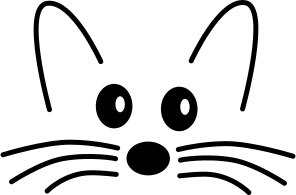
\includegraphics[width=1.4em]{squeak-logo}}}
\iftoshelse{
	\usepackage{marginnote}
		\renewcommand*{\marginfont}{\footnotesize}
	\newcommand{\vartriangleout}{\ifthenelse{\isodd{\thepage}}{\vartriangleright}{\vartriangleleft}}
	\newcommand{\dothisicon}{\fcolorbox{blue!65}{white}{\highlight{$\vartriangleout$}}}
	\newcommand{\dothis}[1]{%
		\noindent\par\noindent
		{\reversemarginpar
			\marginnote{\fcolorbox{blue!65}{white}{\highlight{$\vartriangleout$}}}}
		%\MarginLabel{do this}
		\noindent\emph{#1}
		\nopagebreak}
}{
	\newcommand{\dothisicon}{\raisebox{-.5ex}{
\includegraphics[height=1.2em]{pharo}}}
	\newcommand{\dothis}[1]{%
		\medskip
		\noindent\dothisicon
		\ifx#1\empty\else\quad\emph{#1}\fi
		\par\smallskip\nopagebreak}
}
%===> NEW VERSION <===
% NB: To use this in an individual chapter, you must set:
%\graphicspath{{figures/} {../figures/}}
% at the head of the chapter.  Don't forget the final /
%=============================================================
%:Reader hints (hint)
%
% Indicates a non-obvious consequence 
\newcommand{\hint}[1]{\vspace{1ex}\noindent\fbox{\textsc{Hint}} \emph{#1}}
%=================================================================
% graphics for Morphic handles
\newcommand{\grabHandle}{\raisebox{-0.2ex}{
\includegraphics[width=1em]{blackHandle}}}
\newcommand{\moveHandle}{\raisebox{-0.2ex}{
\includegraphics[width=1em]{moveHandle}}}
\newcommand{\debugHandle}{\raisebox{-0.2ex}{
\includegraphics[width=1em]{debugHandle}}}
%=============================================================
%:Highlighting Important stuff (doublebox)
%
% From Seaside book ...
\newsavebox{\SavedText}
\newlength{\InnerBoxRule}\setlength{\InnerBoxRule}{.75\fboxrule}
\newlength{\OuterBoxRule}\setlength{\OuterBoxRule}{1.5\fboxrule}
\newlength{\BoxSeparation}\setlength{\BoxSeparation}{1.5\fboxrule}
\addtolength{\BoxSeparation}{.5pt}
\newlength{\SaveBoxSep}\setlength{\SaveBoxSep}{2\fboxsep}
%
\newenvironment{doublebox}{\begin{lrbox}{\SavedText}
    \begin{minipage}{.75\textwidth}}
    {\end{minipage}\end{lrbox}\begin{center}
    \setlength{\fboxsep}{\BoxSeparation}\setlength{\fboxrule}{\OuterBoxRule}
    \fbox{\setlength{\fboxsep}{\SaveBoxSep}\setlength{\fboxrule}{\InnerBoxRule}%
      \fbox{\usebox{\SavedText}}}
  \end{center}}
% Use this:
\newcommand{\important}[1]{\begin{doublebox}#1\end{doublebox}}
%=============================================================
%:Section depth
\setcounter{secnumdepth}{2}
%% for this to happen start the file with
%\ifx\wholebook\relax\else
%\input{../common.tex}
%\begin{document}
%\fi
% and terminate by
% \ifx\wholebook\relax\else\end{document}\fi

\DeclareGraphicsExtensions{.pdf, .jpg, .png}
%=============================================================
%:PDF setup
\hypersetup{
%   a4paper,
%   pdfstartview=FitV,
%   colorlinks,
%   linkcolor=darkblue,
%   citecolor=darkblue,
   pdftitle={Pharo by Example},
   pdfauthor={Andrew P. Black, St\'ephane Ducasse,	Oscar Nierstrasz,
Damien Pollet},
   pdfkeywords={Smalltalk, Squeak, Object-Oriented Programming, OOP},
   pdfsubject={Computer Science}
}
%=============================================================
%:Page layout and appearance
%
% \renewcommand{\headrulewidth}{0pt}
\renewcommand{\chaptermark}[1]{\markboth{#1}{}}
\renewcommand{\sectionmark}[1]{\markright{\thesection\ #1}}
\renewpagestyle{plain}[\small\itshape]{%
	\setheadrule{0pt}%
	\sethead[][][]{}{}{}%
	\setfoot[][][]{}{}{}}
\renewpagestyle{headings}[\small\itshape]{%
	\setheadrule{0pt}%
	\setmarks{chapter}{section}%
	\sethead[\thepage][][\chaptertitle]{\sectiontitle}{}{\thepage}%
	\setfoot[][][]{}{}{}}
%=============================================================
%:Title section setup and TOC numbering depth
\setcounter{secnumdepth}{1}
\setcounter{tocdepth}{1}
\titleformat{\part}[display]{\centering}{\huge\partname\ \thepart}{1em}{\Huge\textbf}[]
\titleformat{\chapter}[display]{}{\huge\chaptertitlename\ \thechapter}{1em}{\Huge\raggedright\textbf}[]
\titlecontents{part}[3pc]{%
		\pagebreak[2]\addvspace{1em plus.4em minus.2em}%
		\leavevmode\large\bfseries}
	{\contentslabel{3pc}}{\hspace*{-3pc}}
	{}[\nopagebreak]
\titlecontents{chapter}[3pc]{%
		\pagebreak[0]\addvspace{1em plus.2em minus.2em}%
		\leavevmode\bfseries}
	{\contentslabel{3pc}}{}
	{\hfill\contentspage}[\nopagebreak]
\dottedcontents{section}[3pc]{}{3pc}{1pc}
\dottedcontents{subsection}[3pc]{}{0pc}{1pc}
% \dottedcontents{subsection}[4.5em]{}{0pt}{1pc}
% Make \cleardoublepage insert really blank pages http://www.tex.ac.uk/cgi-bin/texfaq2html?label=reallyblank
\let\origdoublepage\cleardoublepage
\newcommand{\clearemptydoublepage}{%
  \clearpage
  {\pagestyle{empty}\origdoublepage}}
\let\cleardoublepage\clearemptydoublepage % see http://www.tex.ac.uk/cgi-bin/texfaq2html?label=patch
%=============================================================
%:FAQ macros (for FAQ chapter)
\newtheorem{faq}{FAQ}
\newcommand{\answer}{\paragraph{Answer}\ }
%=============================================================
%:Listings package configuration
% \newcommand{\caret}{\makebox{\raisebox{0.4ex}{\footnotesize{$\wedge$}}}}
\newcommand{\caret}{\^\,}
\newcommand{\escape}{{\sf \textbackslash}}
\definecolor{source}{gray}{0.95}
\usepackage{listings}
\lstdefinelanguage{Smalltalk}{
%  morekeywords={self,super,true,false,nil,thisContext}, % This is overkill
  morestring=[d]',
  morecomment=[s]{"}{"},
  alsoletter={\#:},
  escapechar={!},
  literate=
    {BANG}{!}1
    {CARET}{\^}1
    {UNDERSCORE}{\_}1
    {\\st}{Smalltalk}9 % convenience -- in case \st occurs in code
    % {'}{{\textquotesingle}}1 % replaced by upquote=true in \lstset
    {_}{{$\leftarrow$}}1
    {>>>}{{\sep}}1
    {^}{{$\uparrow$}}1
    {~}{{$\sim$}}1
    {-}{{\texttt{-}}}1 %{\textminus}}1 %{-}{\hspace{-0.13em}}{-}}1  % the goal is to make - the same width as +
    % {+}{\sf+}1 %{\raisebox{0.08ex}{+}}}1      % and to raise + off the baseline to match -
    {-->}{{\quad$\longrightarrow$\quad}}3
	, % Don't forget the comma at the end!
  tabsize=4
}[keywords,comments,strings]

\lstset{language=Smalltalk,
	basicstyle=\sffamily,
	keywordstyle=\color{black}\bfseries,
	% stringstyle=\ttfamily, % Ugly! do we really want this? -- on
	mathescape=true,
	showstringspaces=false,
	keepspaces=true,
	breaklines=true,
	breakautoindent=true,
	backgroundcolor=\color{source},
	lineskip={-1pt}, % Ugly hack
	upquote=true, % straight quote; requires textcomp package
	columns=fullflexible} % no fixed width fonts
% In-line code (literal)
% Normally use this for all in-line code:
\newcommand{\ct}{\lstinline[mathescape=false,backgroundcolor=\color{white},basicstyle={\sffamily\upshape}]}
% apb 2007.8.28 added the \upshape declaration to avoid getting italicized code in \dothis{ } sections.
% In-line code (latex enabled)
% Use this only in special situations where \ct does not work
% (within section headings ...):
\newcommand{\lct}[1]{{\textsf{\textup{#1}}}}
% Use these for system categories and protocols:
\newcommand{\scat}[1]{\emph{\textsf{#1}}\xspace}
\newcommand{\pkg}[1]{\emph{\textsf{#1}}\xspace}
\newcommand{\prot}[1]{\emph{\textsf{#1}}\xspace}
% Code environments
% NB: the arg is for tests
% Only code and example environments may be tests
\lstnewenvironment{code}[1]{%
	\lstset{%
		% frame=lines,
		frame=single,
		framerule=0pt,
		mathescape=false
	}
}{}
\def\ignoredollar#1{}
%=============================================================
%:Code environments (method, script ...)
% NB: the third arg is for tests
% Only code and example environments may be tests
\lstnewenvironment{example}[3][defaultlabel]{%
	\renewcommand{\lstlistingname}{Example}%
	\lstset{
		% frame=lines,
		frame=single,
		framerule=0pt,
		mathescape=false,
		caption={\emph{#2}},
		label={eg:#1}
	}
}{}
\lstnewenvironment{script}[2][defaultlabel]{%
\renewcommand{\lstlistingname}{Script}%
	\lstset{
		% frame=lines,
		frame=single,
		framerule=0pt,
		mathescape=false,
		name={Script},
		caption={\emph{#2}},
		label={scr:#1}
	}
}{}
\lstnewenvironment{method}[2][defaultlabel]{%
	\renewcommand{\lstlistingname}{Method}%
	\lstset{
		% frame=lines,
		frame=single,
		framerule=0pt,
		mathescape=false,
		name={Method},
		caption={\emph{#2}},
		label={mth:#1}
	}
}{}
\lstnewenvironment{methods}[2][defaultlabel]{% just for multiple methods at once
	\renewcommand{\lstlistingname}{Methods}%
	\lstset{
		% frame=lines,
		frame=single,
		framerule=0pt,
		mathescape=false,
		name={Method},
		caption={\emph{#2}},
		label={mth:#1}
	}
}{}
\lstnewenvironment{numMethod}[2][defaultlabel]{%
	\renewcommand{\lstlistingname}{Method}%
	\lstset{
		numbers=left,
		numberstyle={\tiny\sffamily},
		% frame=lines,
		frame=single,
		framerule=0pt,
		mathescape=false,
		name={Method},
		caption={\emph{#2}},
		label={mth:#1}
	}
}{}
\lstnewenvironment{classdef}[2][defaultlabel]{%
	\renewcommand{\lstlistingname}{Class}%
	\lstset{
		% frame=lines,
		frame=single,
		framerule=0pt,
		mathescape=false,
		name={Class},
		caption={\emph{#2}},
		label={cls:#1}
	}
}{}
%=============================================================
%:Reserving space
% Usually need one more line than the actual lines of code
\newcommand{\needlines}[1]{\Needspace{#1\baselineskip}}
%=============================================================
%:Indexing macros
% Macros ending with "ind" generate text as well as an index entry
% Macros ending with "index" *only* generate an index entry
\newcommand{\ind}[1]{\index{#1}#1\xspace} % plain text
\newcommand{\subind}[2]{\index{#1!#2}#2\xspace} % show #2, subindex under #1
\newcommand{\emphind}[1]{\index{#1}\emph{#1}\xspace} % emph #1
\newcommand{\emphsubind}[2]{\index{#1!#2}\emph{#2}\xspace} % show emph #2, subindex inder #1
\newcommand{\scatind}[1]{\index{#1@\textsf{#1} (category)}\scat{#1}} % category
\newcommand{\pkgind}[1]{\index{#1@\textsf{#1} (package)}\pkg{#1}} % package
\newcommand{\protind}[1]{\index{#1@\textsf{#1} (protocol)}\prot{#1}} % protocol
\newcommand{\clsind}[1]{\index{#1@\textsf{#1} (class)}\ct{#1}\xspace}
% \newcommand{\clsind}[1]{\index{#1!\#@(class)}\ct{#1}\xspace} % class
\newcommand{\clsindplural}[1]{\index{#1!\#@(class)}\ct{#1}s\xspace} % class
\newcommand{\cvind}[1]{\index{#1@\textsf{#1} (class variable)}\ct{#1}\xspace} % class var
\newcommand{\glbind}[1]{\index{#1@\textsf{#1} (global)}\ct{#1}\xspace} % global
\newcommand{\patind}[1]{\index{#1@#1 (pattern)}\ct{#1}\xspace} % pattern
\newcommand{\pvind}[1]{\index{#1@\textsf{#1} (pseudo variable)}\ct{#1}\xspace} % pseudo var
\newcommand{\clsmthind}[2]{\index{#1!#2@\ct{#2}}\ct{#1>>>#2}\xspace} % class + method name
\newcommand{\mthind}[2]{\index{#1!#2@\ct{#2}}\ct{#2}\xspace} % show method name only
\newcommand{\lmthind}[2]{\index{#1!#2@\ct{#2}}\lct{#2}\xspace} % show method name only
\newcommand{\cmind}[2]{\index{#1!#2@\ct{#2}}\ct{#1>>>#2}\xspace} % show class>>method
\newcommand{\lcmind}[2]{\index{#1!#2@\ct{#2}}\lct{#1>>>#2}\xspace} % show class>>method
\newcommand{\toolsflapind}{\index{Tools flap}\toolsflap} % index tools flap
% The following only generate an index entry:
% \newcommand{\clsindex}[1]{\index{#1@\textsf{#1} (class)}}
\newcommand{\clsindex}[1]{\index{#1!\#@(class)}} % class
\newcommand{\mthindex}[2]{\index{#1!#2@\ct{#2}}} % method
\newcommand{\cmindex}[2]{\index{#1!#2@\ct{#2}}} % class>>method
\newcommand{\cvindex}[1]{\index{#1@\textsf{#1} (class variable)}} % class var
\newcommand{\glbindex}[1]{\index{#1@\textsf{#1} (global)}}% global
\newcommand{\pvindex}[1]{\index{#1@\textsf{#1} (pseudo variable)}}% pseudo var
\newcommand{\seeindex}[2]{\index{#1|see{#2}}} % #1, see #2
\newcommand{\scatindex}[1]{\index{#1@\textsf{#1} (category)}} % category
\newcommand{\pkgindex}[1]{\index{#1@\textsf{#1} (package)}} % package
\newcommand{\protindex}[1]{\index{#1@\textsf{#1} (protocol)}} % protocol
% How can we have the main entry page numbers in bold yet not break the hyperlink?
\newcommand{\boldidx}[1]{{\bf #1}} % breaks hyperlink
%\newcommand{\indmain}[1]{\index{#1|boldidx}#1\xspace} % plain text, main entry
%\newcommand{\emphsubindmain}[2]{\index{#1!#2|boldidx}\emph{#2}\xspace} % subindex, main entry
%\newcommand{\subindmain}[2]{\index{#1!#2|boldidx}#2\xspace} % subindex, main entry
%\newcommand{\clsindmain}[1]{\index{#1@\textsf{#1} (class)|boldidx}\ct{#1}\xspace}
%\newcommand{\clsindmain}[1]{\index{#1!\#@(class)|boldidx}\ct{#1}\xspace} % class main
%\newcommand{\indexmain}[1]{\index{#1|boldidx}} % main index entry only
\newcommand{\indmain}[1]{\index{#1}#1\xspace} % The main index entry for this item
\newcommand{\emphsubindmain}[2]{\index{#1!#2}\emph{#2}\xspace} % subindex, main entry
\newcommand{\subindmain}[2]{\index{#1!#2}#2\xspace} % subindex, main entry
%\newcommand{\clsindmain}[1]{\index{#1@\textsf{#1} (class)}\ct{#1}\xspace}
\newcommand{\clsindmain}[1]{\index{#1!\#@(class)}\ct{#1}\xspace} % class main
\newcommand{\clsindexmain}[1]{\index{#1!\#@(class)}} % class main index only
\newcommand{\indexmain}[1]{\index{#1}} 
%=============================================================
%:Code macros
% some constants
\newcommand{\codesize}{\small}
\newcommand{\codefont}{\sffamily}
%\newcommand{\cat}[1]{\textit{In category #1}}%%To remove later
\newlength{\scriptindent}
\setlength{\scriptindent}{.3cm}
%% Method presentation constants
\newlength{\methodindent}
\newlength{\methodwordlength}
\newlength{\aftermethod}
\setlength{\methodindent}{0.2cm}
\settowidth{\methodwordlength}{\ M\'ethode\ }
%=============================================================
%:Smalltalk macros
%\newcommand{\sep}{{$\gg$}}
\newcommand{\sep}{\mbox{>>}}
\newcommand{\self}{\lct{self}\xspace}
\newcommand{\super}{\lct{super}\xspace}
\newcommand{\nil}{\lct{nil}\xspace}
%=============================================================
% be less conservative about float placement
% these commands are from http://www.tex.ac.uk/cgi-bin/texfaq2html?label=floats
\renewcommand{\topfraction}{.9}
\renewcommand{\bottomfraction}{.9}
\renewcommand{\textfraction}{.1}
\renewcommand{\floatpagefraction}{.85}
\renewcommand{\dbltopfraction}{.66}
\renewcommand{\dblfloatpagefraction}{.85}
\setcounter{topnumber}{9}
\setcounter{bottomnumber}{9}
\setcounter{totalnumber}{20}
\setcounter{dbltopnumber}{9}
%=============================================================
% Give information from each chapter's author
\newcommand{\contact}[2]{\textbf{#1} \textsf{(#2)}}

\newcommand{\chapterauthor}[1]{\emph{with the participation of:\\#1}\\}

\newcommand{\authornoury}{\contact{Noury Bouraqadi}{bouraqadi@gmail.com}}
\newcommand{\authordamienc}{\contact{Damien Cassou}{damien.cassou@gmail.com}}
\newcommand{\authoroscar}{\contact{Oscar Nierstrasz}{oscar.nierstrasz@acm.org}}
\newcommand{\authorsteph}{\contact{St\'ephane Ducasse}{stephane.ducasse@inria.fr}}
\newcommand{\authoralex}{\contact{Alexandre Bergel}{alexandre@bergel.eu}}
\newcommand{\authorolivier}{\contact{Olivier Auverlot}{olivier.auverlot@inria.fr}}
\newcommand{\authornicolas}{\contact{Nicolas Cellier}{nicolas.cellier.aka.nice@gmail.com}}
\newcommand{\authormarcus}{\contact{Marcus Denker}{marcus.denker@inria.fr}}
\newcommand{\authoralain}{\contact{Alain Plantec}{alain.plantec@univ-brest.fr}}
\newcommand{\authordale}{\contact{Dale Henrichs}{dale.henrichs@gemstone.com}}
\newcommand{\authormariano}{\contact{Mariano Martinez Peck}{marianopeck@gmail.com}}
\newcommand{\authorsven}{\contact{Sven Van Caekenberghe}{sven@beta9.be}}
\newcommand{\authorlukas}{\contact{Lukas Renggli}{renggli@gmail.com}}

%=============================================================
% apb doesn't like paragraphs to run in to each other without a break
\parskip 1ex
%=============================================================
%:Stuff to check, merge or deprecate
%\setlength{\marginparsep}{2mm}
%\renewcommand{\baselinestretch}{1.1}
%=============================================================

%\begin{document}
%\fi
% and terminate by
% \ifx\wholebook\relax\else\end{document}\fi

\DeclareGraphicsExtensions{.pdf, .jpg, .png}
%=============================================================
%:PDF setup
\hypersetup{
%   a4paper,
%   pdfstartview=FitV,
%   colorlinks,
%   linkcolor=darkblue,
%   citecolor=darkblue,
   pdftitle={Pharo by Example},
   pdfauthor={Andrew P. Black, St\'ephane Ducasse,	Oscar Nierstrasz,
Damien Pollet},
   pdfkeywords={Smalltalk, Squeak, Object-Oriented Programming, OOP},
   pdfsubject={Computer Science}
}
%=============================================================
%:Page layout and appearance
%
% \renewcommand{\headrulewidth}{0pt}
\renewcommand{\chaptermark}[1]{\markboth{#1}{}}
\renewcommand{\sectionmark}[1]{\markright{\thesection\ #1}}
\renewpagestyle{plain}[\small\itshape]{%
	\setheadrule{0pt}%
	\sethead[][][]{}{}{}%
	\setfoot[][][]{}{}{}}
\renewpagestyle{headings}[\small\itshape]{%
	\setheadrule{0pt}%
	\setmarks{chapter}{section}%
	\sethead[\thepage][][\chaptertitle]{\sectiontitle}{}{\thepage}%
	\setfoot[][][]{}{}{}}
%=============================================================
%:Title section setup and TOC numbering depth
\setcounter{secnumdepth}{1}
\setcounter{tocdepth}{1}
\titleformat{\part}[display]{\centering}{\huge\partname\ \thepart}{1em}{\Huge\textbf}[]
\titleformat{\chapter}[display]{}{\huge\chaptertitlename\ \thechapter}{1em}{\Huge\raggedright\textbf}[]
\titlecontents{part}[3pc]{%
		\pagebreak[2]\addvspace{1em plus.4em minus.2em}%
		\leavevmode\large\bfseries}
	{\contentslabel{3pc}}{\hspace*{-3pc}}
	{}[\nopagebreak]
\titlecontents{chapter}[3pc]{%
		\pagebreak[0]\addvspace{1em plus.2em minus.2em}%
		\leavevmode\bfseries}
	{\contentslabel{3pc}}{}
	{\hfill\contentspage}[\nopagebreak]
\dottedcontents{section}[3pc]{}{3pc}{1pc}
\dottedcontents{subsection}[3pc]{}{0pc}{1pc}
% \dottedcontents{subsection}[4.5em]{}{0pt}{1pc}
% Make \cleardoublepage insert really blank pages http://www.tex.ac.uk/cgi-bin/texfaq2html?label=reallyblank
\let\origdoublepage\cleardoublepage
\newcommand{\clearemptydoublepage}{%
  \clearpage
  {\pagestyle{empty}\origdoublepage}}
\let\cleardoublepage\clearemptydoublepage % see http://www.tex.ac.uk/cgi-bin/texfaq2html?label=patch
%=============================================================
%:FAQ macros (for FAQ chapter)
\newtheorem{faq}{FAQ}
\newcommand{\answer}{\paragraph{Answer}\ }
%=============================================================
%:Listings package configuration
% \newcommand{\caret}{\makebox{\raisebox{0.4ex}{\footnotesize{$\wedge$}}}}
\newcommand{\caret}{\^\,}
\newcommand{\escape}{{\sf \textbackslash}}
\definecolor{source}{gray}{0.95}
\usepackage{listings}
\lstdefinelanguage{Smalltalk}{
%  morekeywords={self,super,true,false,nil,thisContext}, % This is overkill
  morestring=[d]',
  morecomment=[s]{"}{"},
  alsoletter={\#:},
  escapechar={!},
  literate=
    {BANG}{!}1
    {CARET}{\^}1
    {UNDERSCORE}{\_}1
    {\\st}{Smalltalk}9 % convenience -- in case \st occurs in code
    % {'}{{\textquotesingle}}1 % replaced by upquote=true in \lstset
    {_}{{$\leftarrow$}}1
    {>>>}{{\sep}}1
    {^}{{$\uparrow$}}1
    {~}{{$\sim$}}1
    {-}{{\texttt{-}}}1 %{\textminus}}1 %{-}{\hspace{-0.13em}}{-}}1  % the goal is to make - the same width as +
    % {+}{\sf+}1 %{\raisebox{0.08ex}{+}}}1      % and to raise + off the baseline to match -
    {-->}{{\quad$\longrightarrow$\quad}}3
	, % Don't forget the comma at the end!
  tabsize=4
}[keywords,comments,strings]

\lstset{language=Smalltalk,
	basicstyle=\sffamily,
	keywordstyle=\color{black}\bfseries,
	% stringstyle=\ttfamily, % Ugly! do we really want this? -- on
	mathescape=true,
	showstringspaces=false,
	keepspaces=true,
	breaklines=true,
	breakautoindent=true,
	backgroundcolor=\color{source},
	lineskip={-1pt}, % Ugly hack
	upquote=true, % straight quote; requires textcomp package
	columns=fullflexible} % no fixed width fonts
% In-line code (literal)
% Normally use this for all in-line code:
\newcommand{\ct}{\lstinline[mathescape=false,backgroundcolor=\color{white},basicstyle={\sffamily\upshape}]}
% apb 2007.8.28 added the \upshape declaration to avoid getting italicized code in \dothis{ } sections.
% In-line code (latex enabled)
% Use this only in special situations where \ct does not work
% (within section headings ...):
\newcommand{\lct}[1]{{\textsf{\textup{#1}}}}
% Use these for system categories and protocols:
\newcommand{\scat}[1]{\emph{\textsf{#1}}\xspace}
\newcommand{\pkg}[1]{\emph{\textsf{#1}}\xspace}
\newcommand{\prot}[1]{\emph{\textsf{#1}}\xspace}
% Code environments
% NB: the arg is for tests
% Only code and example environments may be tests
\lstnewenvironment{code}[1]{%
	\lstset{%
		% frame=lines,
		frame=single,
		framerule=0pt,
		mathescape=false
	}
}{}
\def\ignoredollar#1{}
%=============================================================
%:Code environments (method, script ...)
% NB: the third arg is for tests
% Only code and example environments may be tests
\lstnewenvironment{example}[3][defaultlabel]{%
	\renewcommand{\lstlistingname}{Example}%
	\lstset{
		% frame=lines,
		frame=single,
		framerule=0pt,
		mathescape=false,
		caption={\emph{#2}},
		label={eg:#1}
	}
}{}
\lstnewenvironment{script}[2][defaultlabel]{%
\renewcommand{\lstlistingname}{Script}%
	\lstset{
		% frame=lines,
		frame=single,
		framerule=0pt,
		mathescape=false,
		name={Script},
		caption={\emph{#2}},
		label={scr:#1}
	}
}{}
\lstnewenvironment{method}[2][defaultlabel]{%
	\renewcommand{\lstlistingname}{Method}%
	\lstset{
		% frame=lines,
		frame=single,
		framerule=0pt,
		mathescape=false,
		name={Method},
		caption={\emph{#2}},
		label={mth:#1}
	}
}{}
\lstnewenvironment{methods}[2][defaultlabel]{% just for multiple methods at once
	\renewcommand{\lstlistingname}{Methods}%
	\lstset{
		% frame=lines,
		frame=single,
		framerule=0pt,
		mathescape=false,
		name={Method},
		caption={\emph{#2}},
		label={mth:#1}
	}
}{}
\lstnewenvironment{numMethod}[2][defaultlabel]{%
	\renewcommand{\lstlistingname}{Method}%
	\lstset{
		numbers=left,
		numberstyle={\tiny\sffamily},
		% frame=lines,
		frame=single,
		framerule=0pt,
		mathescape=false,
		name={Method},
		caption={\emph{#2}},
		label={mth:#1}
	}
}{}
\lstnewenvironment{classdef}[2][defaultlabel]{%
	\renewcommand{\lstlistingname}{Class}%
	\lstset{
		% frame=lines,
		frame=single,
		framerule=0pt,
		mathescape=false,
		name={Class},
		caption={\emph{#2}},
		label={cls:#1}
	}
}{}
%=============================================================
%:Reserving space
% Usually need one more line than the actual lines of code
\newcommand{\needlines}[1]{\Needspace{#1\baselineskip}}
%=============================================================
%:Indexing macros
% Macros ending with "ind" generate text as well as an index entry
% Macros ending with "index" *only* generate an index entry
\newcommand{\ind}[1]{\index{#1}#1\xspace} % plain text
\newcommand{\subind}[2]{\index{#1!#2}#2\xspace} % show #2, subindex under #1
\newcommand{\emphind}[1]{\index{#1}\emph{#1}\xspace} % emph #1
\newcommand{\emphsubind}[2]{\index{#1!#2}\emph{#2}\xspace} % show emph #2, subindex inder #1
\newcommand{\scatind}[1]{\index{#1@\textsf{#1} (category)}\scat{#1}} % category
\newcommand{\pkgind}[1]{\index{#1@\textsf{#1} (package)}\pkg{#1}} % package
\newcommand{\protind}[1]{\index{#1@\textsf{#1} (protocol)}\prot{#1}} % protocol
\newcommand{\clsind}[1]{\index{#1@\textsf{#1} (class)}\ct{#1}\xspace}
% \newcommand{\clsind}[1]{\index{#1!\#@(class)}\ct{#1}\xspace} % class
\newcommand{\clsindplural}[1]{\index{#1!\#@(class)}\ct{#1}s\xspace} % class
\newcommand{\cvind}[1]{\index{#1@\textsf{#1} (class variable)}\ct{#1}\xspace} % class var
\newcommand{\glbind}[1]{\index{#1@\textsf{#1} (global)}\ct{#1}\xspace} % global
\newcommand{\patind}[1]{\index{#1@#1 (pattern)}\ct{#1}\xspace} % pattern
\newcommand{\pvind}[1]{\index{#1@\textsf{#1} (pseudo variable)}\ct{#1}\xspace} % pseudo var
\newcommand{\clsmthind}[2]{\index{#1!#2@\ct{#2}}\ct{#1>>>#2}\xspace} % class + method name
\newcommand{\mthind}[2]{\index{#1!#2@\ct{#2}}\ct{#2}\xspace} % show method name only
\newcommand{\lmthind}[2]{\index{#1!#2@\ct{#2}}\lct{#2}\xspace} % show method name only
\newcommand{\cmind}[2]{\index{#1!#2@\ct{#2}}\ct{#1>>>#2}\xspace} % show class>>method
\newcommand{\lcmind}[2]{\index{#1!#2@\ct{#2}}\lct{#1>>>#2}\xspace} % show class>>method
\newcommand{\toolsflapind}{\index{Tools flap}\toolsflap} % index tools flap
% The following only generate an index entry:
% \newcommand{\clsindex}[1]{\index{#1@\textsf{#1} (class)}}
\newcommand{\clsindex}[1]{\index{#1!\#@(class)}} % class
\newcommand{\mthindex}[2]{\index{#1!#2@\ct{#2}}} % method
\newcommand{\cmindex}[2]{\index{#1!#2@\ct{#2}}} % class>>method
\newcommand{\cvindex}[1]{\index{#1@\textsf{#1} (class variable)}} % class var
\newcommand{\glbindex}[1]{\index{#1@\textsf{#1} (global)}}% global
\newcommand{\pvindex}[1]{\index{#1@\textsf{#1} (pseudo variable)}}% pseudo var
\newcommand{\seeindex}[2]{\index{#1|see{#2}}} % #1, see #2
\newcommand{\scatindex}[1]{\index{#1@\textsf{#1} (category)}} % category
\newcommand{\pkgindex}[1]{\index{#1@\textsf{#1} (package)}} % package
\newcommand{\protindex}[1]{\index{#1@\textsf{#1} (protocol)}} % protocol
% How can we have the main entry page numbers in bold yet not break the hyperlink?
\newcommand{\boldidx}[1]{{\bf #1}} % breaks hyperlink
%\newcommand{\indmain}[1]{\index{#1|boldidx}#1\xspace} % plain text, main entry
%\newcommand{\emphsubindmain}[2]{\index{#1!#2|boldidx}\emph{#2}\xspace} % subindex, main entry
%\newcommand{\subindmain}[2]{\index{#1!#2|boldidx}#2\xspace} % subindex, main entry
%\newcommand{\clsindmain}[1]{\index{#1@\textsf{#1} (class)|boldidx}\ct{#1}\xspace}
%\newcommand{\clsindmain}[1]{\index{#1!\#@(class)|boldidx}\ct{#1}\xspace} % class main
%\newcommand{\indexmain}[1]{\index{#1|boldidx}} % main index entry only
\newcommand{\indmain}[1]{\index{#1}#1\xspace} % The main index entry for this item
\newcommand{\emphsubindmain}[2]{\index{#1!#2}\emph{#2}\xspace} % subindex, main entry
\newcommand{\subindmain}[2]{\index{#1!#2}#2\xspace} % subindex, main entry
%\newcommand{\clsindmain}[1]{\index{#1@\textsf{#1} (class)}\ct{#1}\xspace}
\newcommand{\clsindmain}[1]{\index{#1!\#@(class)}\ct{#1}\xspace} % class main
\newcommand{\clsindexmain}[1]{\index{#1!\#@(class)}} % class main index only
\newcommand{\indexmain}[1]{\index{#1}} 
%=============================================================
%:Code macros
% some constants
\newcommand{\codesize}{\small}
\newcommand{\codefont}{\sffamily}
%\newcommand{\cat}[1]{\textit{In category #1}}%%To remove later
\newlength{\scriptindent}
\setlength{\scriptindent}{.3cm}
%% Method presentation constants
\newlength{\methodindent}
\newlength{\methodwordlength}
\newlength{\aftermethod}
\setlength{\methodindent}{0.2cm}
\settowidth{\methodwordlength}{\ M\'ethode\ }
%=============================================================
%:Smalltalk macros
%\newcommand{\sep}{{$\gg$}}
\newcommand{\sep}{\mbox{>>}}
\newcommand{\self}{\lct{self}\xspace}
\newcommand{\super}{\lct{super}\xspace}
\newcommand{\nil}{\lct{nil}\xspace}
%=============================================================
% be less conservative about float placement
% these commands are from http://www.tex.ac.uk/cgi-bin/texfaq2html?label=floats
\renewcommand{\topfraction}{.9}
\renewcommand{\bottomfraction}{.9}
\renewcommand{\textfraction}{.1}
\renewcommand{\floatpagefraction}{.85}
\renewcommand{\dbltopfraction}{.66}
\renewcommand{\dblfloatpagefraction}{.85}
\setcounter{topnumber}{9}
\setcounter{bottomnumber}{9}
\setcounter{totalnumber}{20}
\setcounter{dbltopnumber}{9}
%=============================================================
% Give information from each chapter's author
\newcommand{\contact}[2]{\textbf{#1} \textsf{(#2)}}

\newcommand{\chapterauthor}[1]{\emph{with the participation of:\\#1}\\}

\newcommand{\authornoury}{\contact{Noury Bouraqadi}{bouraqadi@gmail.com}}
\newcommand{\authordamienc}{\contact{Damien Cassou}{damien.cassou@gmail.com}}
\newcommand{\authoroscar}{\contact{Oscar Nierstrasz}{oscar.nierstrasz@acm.org}}
\newcommand{\authorsteph}{\contact{St\'ephane Ducasse}{stephane.ducasse@inria.fr}}
\newcommand{\authoralex}{\contact{Alexandre Bergel}{alexandre@bergel.eu}}
\newcommand{\authorolivier}{\contact{Olivier Auverlot}{olivier.auverlot@inria.fr}}
\newcommand{\authornicolas}{\contact{Nicolas Cellier}{nicolas.cellier.aka.nice@gmail.com}}
\newcommand{\authormarcus}{\contact{Marcus Denker}{marcus.denker@inria.fr}}
\newcommand{\authoralain}{\contact{Alain Plantec}{alain.plantec@univ-brest.fr}}
\newcommand{\authordale}{\contact{Dale Henrichs}{dale.henrichs@gemstone.com}}
\newcommand{\authormariano}{\contact{Mariano Martinez Peck}{marianopeck@gmail.com}}
\newcommand{\authorsven}{\contact{Sven Van Caekenberghe}{sven@beta9.be}}
\newcommand{\authorlukas}{\contact{Lukas Renggli}{renggli@gmail.com}}

%=============================================================
% apb doesn't like paragraphs to run in to each other without a break
\parskip 1ex
%=============================================================
%:Stuff to check, merge or deprecate
%\setlength{\marginparsep}{2mm}
%\renewcommand{\baselinestretch}{1.1}
%=============================================================

%\begin{document}
%\fi
% and terminate by
% \ifx\wholebook\relax\else\end{document}\fi

\DeclareGraphicsExtensions{.pdf, .jpg, .png}
%=============================================================
%:PDF setup
\hypersetup{
%   a4paper,
%   pdfstartview=FitV,
%   colorlinks,
%   linkcolor=darkblue,
%   citecolor=darkblue,
   pdftitle={Pharo by Example},
   pdfauthor={Andrew P. Black, St\'ephane Ducasse,	Oscar Nierstrasz,
Damien Pollet},
   pdfkeywords={Smalltalk, Squeak, Object-Oriented Programming, OOP},
   pdfsubject={Computer Science}
}
%=============================================================
%:Page layout and appearance
%
% \renewcommand{\headrulewidth}{0pt}
\renewcommand{\chaptermark}[1]{\markboth{#1}{}}
\renewcommand{\sectionmark}[1]{\markright{\thesection\ #1}}
\renewpagestyle{plain}[\small\itshape]{%
	\setheadrule{0pt}%
	\sethead[][][]{}{}{}%
	\setfoot[][][]{}{}{}}
\renewpagestyle{headings}[\small\itshape]{%
	\setheadrule{0pt}%
	\setmarks{chapter}{section}%
	\sethead[\thepage][][\chaptertitle]{\sectiontitle}{}{\thepage}%
	\setfoot[][][]{}{}{}}
%=============================================================
%:Title section setup and TOC numbering depth
\setcounter{secnumdepth}{1}
\setcounter{tocdepth}{1}
\titleformat{\part}[display]{\centering}{\huge\partname\ \thepart}{1em}{\Huge\textbf}[]
\titleformat{\chapter}[display]{}{\huge\chaptertitlename\ \thechapter}{1em}{\Huge\raggedright\textbf}[]
\titlecontents{part}[3pc]{%
		\pagebreak[2]\addvspace{1em plus.4em minus.2em}%
		\leavevmode\large\bfseries}
	{\contentslabel{3pc}}{\hspace*{-3pc}}
	{}[\nopagebreak]
\titlecontents{chapter}[3pc]{%
		\pagebreak[0]\addvspace{1em plus.2em minus.2em}%
		\leavevmode\bfseries}
	{\contentslabel{3pc}}{}
	{\hfill\contentspage}[\nopagebreak]
\dottedcontents{section}[3pc]{}{3pc}{1pc}
\dottedcontents{subsection}[3pc]{}{0pc}{1pc}
% \dottedcontents{subsection}[4.5em]{}{0pt}{1pc}
% Make \cleardoublepage insert really blank pages http://www.tex.ac.uk/cgi-bin/texfaq2html?label=reallyblank
\let\origdoublepage\cleardoublepage
\newcommand{\clearemptydoublepage}{%
  \clearpage
  {\pagestyle{empty}\origdoublepage}}
\let\cleardoublepage\clearemptydoublepage % see http://www.tex.ac.uk/cgi-bin/texfaq2html?label=patch
%=============================================================
%:FAQ macros (for FAQ chapter)
\newtheorem{faq}{FAQ}
\newcommand{\answer}{\paragraph{Answer}\ }
%=============================================================
%:Listings package configuration
% \newcommand{\caret}{\makebox{\raisebox{0.4ex}{\footnotesize{$\wedge$}}}}
\newcommand{\caret}{\^\,}
\newcommand{\escape}{{\sf \textbackslash}}
\definecolor{source}{gray}{0.95}
\usepackage{listings}
\lstdefinelanguage{Smalltalk}{
%  morekeywords={self,super,true,false,nil,thisContext}, % This is overkill
  morestring=[d]',
  morecomment=[s]{"}{"},
  alsoletter={\#:},
  escapechar={!},
  literate=
    {BANG}{!}1
    {CARET}{\^}1
    {UNDERSCORE}{\_}1
    {\\st}{Smalltalk}9 % convenience -- in case \st occurs in code
    % {'}{{\textquotesingle}}1 % replaced by upquote=true in \lstset
    {_}{{$\leftarrow$}}1
    {>>>}{{\sep}}1
    {^}{{$\uparrow$}}1
    {~}{{$\sim$}}1
    {-}{{\texttt{-}}}1 %{\textminus}}1 %{-}{\hspace{-0.13em}}{-}}1  % the goal is to make - the same width as +
    % {+}{\sf+}1 %{\raisebox{0.08ex}{+}}}1      % and to raise + off the baseline to match -
    {-->}{{\quad$\longrightarrow$\quad}}3
	, % Don't forget the comma at the end!
  tabsize=4
}[keywords,comments,strings]

\lstset{language=Smalltalk,
	basicstyle=\sffamily,
	keywordstyle=\color{black}\bfseries,
	% stringstyle=\ttfamily, % Ugly! do we really want this? -- on
	mathescape=true,
	showstringspaces=false,
	keepspaces=true,
	breaklines=true,
	breakautoindent=true,
	backgroundcolor=\color{source},
	lineskip={-1pt}, % Ugly hack
	upquote=true, % straight quote; requires textcomp package
	columns=fullflexible} % no fixed width fonts
% In-line code (literal)
% Normally use this for all in-line code:
\newcommand{\ct}{\lstinline[mathescape=false,backgroundcolor=\color{white},basicstyle={\sffamily\upshape}]}
% apb 2007.8.28 added the \upshape declaration to avoid getting italicized code in \dothis{ } sections.
% In-line code (latex enabled)
% Use this only in special situations where \ct does not work
% (within section headings ...):
\newcommand{\lct}[1]{{\textsf{\textup{#1}}}}
% Use these for system categories and protocols:
\newcommand{\scat}[1]{\emph{\textsf{#1}}\xspace}
\newcommand{\pkg}[1]{\emph{\textsf{#1}}\xspace}
\newcommand{\prot}[1]{\emph{\textsf{#1}}\xspace}
% Code environments
% NB: the arg is for tests
% Only code and example environments may be tests
\lstnewenvironment{code}[1]{%
	\lstset{%
		% frame=lines,
		frame=single,
		framerule=0pt,
		mathescape=false
	}
}{}
\def\ignoredollar#1{}
%=============================================================
%:Code environments (method, script ...)
% NB: the third arg is for tests
% Only code and example environments may be tests
\lstnewenvironment{example}[3][defaultlabel]{%
	\renewcommand{\lstlistingname}{Example}%
	\lstset{
		% frame=lines,
		frame=single,
		framerule=0pt,
		mathescape=false,
		caption={\emph{#2}},
		label={eg:#1}
	}
}{}
\lstnewenvironment{script}[2][defaultlabel]{%
\renewcommand{\lstlistingname}{Script}%
	\lstset{
		% frame=lines,
		frame=single,
		framerule=0pt,
		mathescape=false,
		name={Script},
		caption={\emph{#2}},
		label={scr:#1}
	}
}{}
\lstnewenvironment{method}[2][defaultlabel]{%
	\renewcommand{\lstlistingname}{Method}%
	\lstset{
		% frame=lines,
		frame=single,
		framerule=0pt,
		mathescape=false,
		name={Method},
		caption={\emph{#2}},
		label={mth:#1}
	}
}{}
\lstnewenvironment{methods}[2][defaultlabel]{% just for multiple methods at once
	\renewcommand{\lstlistingname}{Methods}%
	\lstset{
		% frame=lines,
		frame=single,
		framerule=0pt,
		mathescape=false,
		name={Method},
		caption={\emph{#2}},
		label={mth:#1}
	}
}{}
\lstnewenvironment{numMethod}[2][defaultlabel]{%
	\renewcommand{\lstlistingname}{Method}%
	\lstset{
		numbers=left,
		numberstyle={\tiny\sffamily},
		% frame=lines,
		frame=single,
		framerule=0pt,
		mathescape=false,
		name={Method},
		caption={\emph{#2}},
		label={mth:#1}
	}
}{}
\lstnewenvironment{classdef}[2][defaultlabel]{%
	\renewcommand{\lstlistingname}{Class}%
	\lstset{
		% frame=lines,
		frame=single,
		framerule=0pt,
		mathescape=false,
		name={Class},
		caption={\emph{#2}},
		label={cls:#1}
	}
}{}
%=============================================================
%:Reserving space
% Usually need one more line than the actual lines of code
\newcommand{\needlines}[1]{\Needspace{#1\baselineskip}}
%=============================================================
%:Indexing macros
% Macros ending with "ind" generate text as well as an index entry
% Macros ending with "index" *only* generate an index entry
\newcommand{\ind}[1]{\index{#1}#1\xspace} % plain text
\newcommand{\subind}[2]{\index{#1!#2}#2\xspace} % show #2, subindex under #1
\newcommand{\emphind}[1]{\index{#1}\emph{#1}\xspace} % emph #1
\newcommand{\emphsubind}[2]{\index{#1!#2}\emph{#2}\xspace} % show emph #2, subindex inder #1
\newcommand{\scatind}[1]{\index{#1@\textsf{#1} (category)}\scat{#1}} % category
\newcommand{\pkgind}[1]{\index{#1@\textsf{#1} (package)}\pkg{#1}} % package
\newcommand{\protind}[1]{\index{#1@\textsf{#1} (protocol)}\prot{#1}} % protocol
\newcommand{\clsind}[1]{\index{#1@\textsf{#1} (class)}\ct{#1}\xspace}
% \newcommand{\clsind}[1]{\index{#1!\#@(class)}\ct{#1}\xspace} % class
\newcommand{\clsindplural}[1]{\index{#1!\#@(class)}\ct{#1}s\xspace} % class
\newcommand{\cvind}[1]{\index{#1@\textsf{#1} (class variable)}\ct{#1}\xspace} % class var
\newcommand{\glbind}[1]{\index{#1@\textsf{#1} (global)}\ct{#1}\xspace} % global
\newcommand{\patind}[1]{\index{#1@#1 (pattern)}\ct{#1}\xspace} % pattern
\newcommand{\pvind}[1]{\index{#1@\textsf{#1} (pseudo variable)}\ct{#1}\xspace} % pseudo var
\newcommand{\clsmthind}[2]{\index{#1!#2@\ct{#2}}\ct{#1>>>#2}\xspace} % class + method name
\newcommand{\mthind}[2]{\index{#1!#2@\ct{#2}}\ct{#2}\xspace} % show method name only
\newcommand{\lmthind}[2]{\index{#1!#2@\ct{#2}}\lct{#2}\xspace} % show method name only
\newcommand{\cmind}[2]{\index{#1!#2@\ct{#2}}\ct{#1>>>#2}\xspace} % show class>>method
\newcommand{\lcmind}[2]{\index{#1!#2@\ct{#2}}\lct{#1>>>#2}\xspace} % show class>>method
\newcommand{\toolsflapind}{\index{Tools flap}\toolsflap} % index tools flap
% The following only generate an index entry:
% \newcommand{\clsindex}[1]{\index{#1@\textsf{#1} (class)}}
\newcommand{\clsindex}[1]{\index{#1!\#@(class)}} % class
\newcommand{\mthindex}[2]{\index{#1!#2@\ct{#2}}} % method
\newcommand{\cmindex}[2]{\index{#1!#2@\ct{#2}}} % class>>method
\newcommand{\cvindex}[1]{\index{#1@\textsf{#1} (class variable)}} % class var
\newcommand{\glbindex}[1]{\index{#1@\textsf{#1} (global)}}% global
\newcommand{\pvindex}[1]{\index{#1@\textsf{#1} (pseudo variable)}}% pseudo var
\newcommand{\seeindex}[2]{\index{#1|see{#2}}} % #1, see #2
\newcommand{\scatindex}[1]{\index{#1@\textsf{#1} (category)}} % category
\newcommand{\pkgindex}[1]{\index{#1@\textsf{#1} (package)}} % package
\newcommand{\protindex}[1]{\index{#1@\textsf{#1} (protocol)}} % protocol
% How can we have the main entry page numbers in bold yet not break the hyperlink?
\newcommand{\boldidx}[1]{{\bf #1}} % breaks hyperlink
%\newcommand{\indmain}[1]{\index{#1|boldidx}#1\xspace} % plain text, main entry
%\newcommand{\emphsubindmain}[2]{\index{#1!#2|boldidx}\emph{#2}\xspace} % subindex, main entry
%\newcommand{\subindmain}[2]{\index{#1!#2|boldidx}#2\xspace} % subindex, main entry
%\newcommand{\clsindmain}[1]{\index{#1@\textsf{#1} (class)|boldidx}\ct{#1}\xspace}
%\newcommand{\clsindmain}[1]{\index{#1!\#@(class)|boldidx}\ct{#1}\xspace} % class main
%\newcommand{\indexmain}[1]{\index{#1|boldidx}} % main index entry only
\newcommand{\indmain}[1]{\index{#1}#1\xspace} % The main index entry for this item
\newcommand{\emphsubindmain}[2]{\index{#1!#2}\emph{#2}\xspace} % subindex, main entry
\newcommand{\subindmain}[2]{\index{#1!#2}#2\xspace} % subindex, main entry
%\newcommand{\clsindmain}[1]{\index{#1@\textsf{#1} (class)}\ct{#1}\xspace}
\newcommand{\clsindmain}[1]{\index{#1!\#@(class)}\ct{#1}\xspace} % class main
\newcommand{\clsindexmain}[1]{\index{#1!\#@(class)}} % class main index only
\newcommand{\indexmain}[1]{\index{#1}} 
%=============================================================
%:Code macros
% some constants
\newcommand{\codesize}{\small}
\newcommand{\codefont}{\sffamily}
%\newcommand{\cat}[1]{\textit{In category #1}}%%To remove later
\newlength{\scriptindent}
\setlength{\scriptindent}{.3cm}
%% Method presentation constants
\newlength{\methodindent}
\newlength{\methodwordlength}
\newlength{\aftermethod}
\setlength{\methodindent}{0.2cm}
\settowidth{\methodwordlength}{\ M\'ethode\ }
%=============================================================
%:Smalltalk macros
%\newcommand{\sep}{{$\gg$}}
\newcommand{\sep}{\mbox{>>}}
\newcommand{\self}{\lct{self}\xspace}
\newcommand{\super}{\lct{super}\xspace}
\newcommand{\nil}{\lct{nil}\xspace}
%=============================================================
% be less conservative about float placement
% these commands are from http://www.tex.ac.uk/cgi-bin/texfaq2html?label=floats
\renewcommand{\topfraction}{.9}
\renewcommand{\bottomfraction}{.9}
\renewcommand{\textfraction}{.1}
\renewcommand{\floatpagefraction}{.85}
\renewcommand{\dbltopfraction}{.66}
\renewcommand{\dblfloatpagefraction}{.85}
\setcounter{topnumber}{9}
\setcounter{bottomnumber}{9}
\setcounter{totalnumber}{20}
\setcounter{dbltopnumber}{9}
%=============================================================
% Give information from each chapter's author
\newcommand{\contact}[2]{\textbf{#1} \textsf{(#2)}}

\newcommand{\chapterauthor}[1]{\emph{with the participation of:\\#1}\\}

\newcommand{\authornoury}{\contact{Noury Bouraqadi}{bouraqadi@gmail.com}}
\newcommand{\authordamienc}{\contact{Damien Cassou}{damien.cassou@gmail.com}}
\newcommand{\authoroscar}{\contact{Oscar Nierstrasz}{oscar.nierstrasz@acm.org}}
\newcommand{\authorsteph}{\contact{St\'ephane Ducasse}{stephane.ducasse@inria.fr}}
\newcommand{\authoralex}{\contact{Alexandre Bergel}{alexandre@bergel.eu}}
\newcommand{\authorolivier}{\contact{Olivier Auverlot}{olivier.auverlot@inria.fr}}
\newcommand{\authornicolas}{\contact{Nicolas Cellier}{nicolas.cellier.aka.nice@gmail.com}}
\newcommand{\authormarcus}{\contact{Marcus Denker}{marcus.denker@inria.fr}}
\newcommand{\authoralain}{\contact{Alain Plantec}{alain.plantec@univ-brest.fr}}
\newcommand{\authordale}{\contact{Dale Henrichs}{dale.henrichs@gemstone.com}}
\newcommand{\authormariano}{\contact{Mariano Martinez Peck}{marianopeck@gmail.com}}
\newcommand{\authorsven}{\contact{Sven Van Caekenberghe}{sven@beta9.be}}
\newcommand{\authorlukas}{\contact{Lukas Renggli}{renggli@gmail.com}}

%=============================================================
% apb doesn't like paragraphs to run in to each other without a break
\parskip 1ex
%=============================================================
%:Stuff to check, merge or deprecate
%\setlength{\marginparsep}{2mm}
%\renewcommand{\baselinestretch}{1.1}
%=============================================================

	\pagestyle{headings}
	\setboolean{lulu}{true}
% --------------------------------------------
% A4:
%	\documentclass[a4paper,11pt,twoside]{book}
%	% $Author$
% $Date$
% $Revision$

% HISTORY:
% 2006-10-31 - Oscar code macros
% ...

%=============================================================
% NB: documentclass must be set in main document.
% Allows book to be generated in multiple formats.
%=============================================================
%:Packages
\usepackage[T1]{fontenc}  %%%%%% really important to get the code directly in the text!
\usepackage{lmodern}
%\usepackage[scaled=0.85]{bookmanx} % needs another scale factor if used with \renewcommand{\sfdefault}{cmbr}
\usepackage{palatino}
\usepackage[scaled=0.85]{helvet}
\usepackage[protrusion,expansion=false]{microtype}
\usepackage{graphicx}
\usepackage{theorem}
\usepackage[english]{babel}
% ON: pdfsync breaks the use of p{width} for tabular columns!
\ifdefined\usepdfsync\usepackage{pdfsync}\fi % Requires texlive 2007
%=============================================================
%:More packages
%Stef should check which ones are used!
%\usepackage{picinpar}
%\usepackage{layout}
%\usepackage{color}
%\usepackage{enum}
%\usepackage{a4wide}
% \usepackage{fancyhdr}
\usepackage{ifthen}
\usepackage{float}
\usepackage{longtable}
\usepackage{makeidx}
\usepackage[nottoc]{tocbibind}
\usepackage{multicol}
\usepackage{booktabs}	% book-style tables
\usepackage{topcapt}	% enables \topcaption
\usepackage{multirow}
\usepackage{tabularx}
%\usepackage[bottom]{footmisc}
\usepackage{xspace}
\usepackage{alltt}
\usepackage{amssymb,textcomp}
\usepackage[usenames,dvipsnames]{color}
%\usepackage{colortbl}
\usepackage[hang]{subfigure}\makeatletter\def\p@subfigure{\thefigure\,}\makeatother
\usepackage{rotating}
\usepackage{enumitem}	% apb: allows more control over tags in enumerations
\usepackage{verbatim}     % for comment environment
\usepackage{varioref}	% for page references that work
\labelformat{footnote}{\thechapter--#1} % to distinguish citations from jurabib
\usepackage{needspace}
\usepackage{isodateo} % enable \isodate
\usepackage[newparttoc]{titlesec}
\usepackage{titletoc}
\usepackage{wrapfig}
\usepackage[
	super,
	citefull=first,
	authorformat={allreversed,and},
	titleformat={commasep,italic}
]{jurabib} % citations as footnotes
\usepackage[
	colorlinks=true,
	linkcolor=black,
	urlcolor=black,
	citecolor=black
]{hyperref}   % should come last
%=============================================================
%:PDF version
\pdfminorversion=3 % Set PDF to 1.3 for Lulu
%=============================================================
%:URL style
\makeatletter
\def\url@leostyle{%
  \@ifundefined{selectfont}{\def\UrlFont{\sf}}{\def\UrlFont{\sffamily}}}
\makeatother
% Now actually use the newly defined style.
\urlstyle{leo}
%=============================================================
%:Booleans
\newboolean{lulu}
\setboolean{lulu}{false}
\newcommand{\ifluluelse}[2]{\ifthenelse{\boolean{lulu}}{#1}{#2}}
%=============================================================
%:Names
\newcommand{\SUnit}{SUnit\xspace}
\newcommand{\sunit}{SUnit\xspace}
\newcommand{\xUnit}{$x$Unit\xspace}
\newcommand{\JUnit}{JUnit\xspace}
\newcommand{\st}{Smalltalk\xspace}
\newcommand{\pharo}{Pharo\xspace} % Use this, not \Pharo
%\newcommand{\sqmap}{SqueakMap\xspace}
\newcommand{\squeak}{Squeak\xspace} % use this, not \Squeak or \sq
\newcommand{\sqsrc}{SqueakSource\xspace}
\newcommand{\sbe}{\url{http://SqueakByExample.org}\xspace}
\newcommand{\pharoweb}{\url{http://pharo-project.org}\xspace}
\newcommand{\pbe}{\url{http://PharoByExample.org}\xspace}
\newcommand{\sba}{\url{http://SquareBracketAssociates.org}\xspace}
\newcommand{\bam}{\lct{Bounc\-ing\-Atoms\-Morph}\xspace}
%=============================================================
%:Markup macros for proof-reading
\usepackage[normalem]{ulem} % for \sout
\usepackage{xcolor}
\newcommand{\ra}{$\rightarrow$}
\newcommand{\ugh}[1]{\textcolor{red}{\uwave{#1}}} % please rephrase
\newcommand{\ins}[1]{\textcolor{blue}{\uline{#1}}} % please insert
\newcommand{\del}[1]{\textcolor{red}{\sout{#1}}} % please delete
\newcommand{\chg}[2]{\textcolor{red}{\sout{#1}}{\ra}\textcolor{blue}{\uline{#2}}} % please change
%=============================================================
%:Editorial comment macros
%\newcommand{\nnbb}[2]{
%    % \fbox{\bfseries\sffamily\scriptsize#1}
%    \fcolorbox{gray}{yellow}{\bfseries\sffamily\scriptsize#1}
%    {\sf\small$\blacktriangleright$\textit{#2}$\blacktriangleleft$}
%   }
\newcommand{\yellowbox}[1]{\fcolorbox{gray}{yellow}{\bfseries\sffamily\scriptsize#1}}
\newcommand{\triangles}[1]{{\sf\small$\blacktriangleright$\textit{#1}$\blacktriangleleft$}}
\newcommand{\nnbb}[2]{\yellowbox{#1} \triangles{#2}}
\newcommand{\fix}{\yellowbox{FIX!}}
\newcommand{\here}{\yellowbox{CONTINUE HERE!}}
% editor macros
\newcommand{\apl}[1]{\nnbb{Alain}{#1}} % Alain
\newcommand{\ab}[1]{\nnbb{Andrew}{#1}} % Black
\newcommand{\sd}[1]{\nnbb{St\'{e}f}{#1}} % Ducasse
\newcommand{\dc}[1]{\nnbb{DamienC}{#1}} % Ducasse
\newcommand{\md}[1]{\nnbb{Marcus}{#1}} % Denker
\newcommand{\on}[1]{\nnbb{Oscar}{#1}} % Nierstrasz
\newcommand{\damien}[1]{\nnbb{Damien}{#1}} % Pollet
\newcommand{\lr}[1]{\nnbb{Lukas}{#1}} % Renggli
\newcommand{\orla}[1]{\nnbb{Orla}{#1}} % Greevy
\newcommand{\alex}[1]{\nnbb{Alex}{#1}} % Bergel
\newcommand{\alx}[1]{\nnbb{Alex}{#1}} % Bergel
\newcommand{\dr}[1]{\nnbb{David}{#1}} % Roethlisberger
\newcommand{\ja}[1]{\nnbb{Jannik}{#1}} % Laval
\newcommand{\jr}[1]{\nnbb{Jorge}{#1}} % Ressia
\newcommand{\jb}[1]{\nnbb{JB}{#1}} % JB
\newcommand{\fp}[1]{\nnbb{Fabrizio}{#1}} % Perin
\newcommand{\michael}[1]{\nnbb{Michael}{#1}} % Davies
\newcommand{\ew}[1]{\nnbb{Erwann}{#1}} % Wernli
\newcommand{\mb}[1]{\nnbb{Martial}{#1}} % Boniou
\newcommand{\hw}[1]{\nnbb{Hernan}{#1}} % Wilkinson
\newcommand{\ben}[1]{\nnbb{Benjamin}{#1}} % Benjamin Van Ryseghem
%=============================================================
%:Abbreviation macros
\newcommand{\ie}{\emph{i.e.},\xspace}
\newcommand{\eg}{\emph{e.g.},\xspace}
\newcommand{\etc}{etc.\xspace}
%=============================================================
%:Cross reference macros
\newcommand{\charef}[1]{Chapter~\ref{cha:#1}\xspace}
\newcommand{\secref}[1]{Section~\ref{sec:#1}\xspace}
\newcommand{\figref}[1]{Figure~\ref{fig:#1}\xspace}
\newcommand{\Figref}[1]{Figure~\ref{fig:#1}\xspace}
\newcommand{\appref}[1]{Appendix~\ref{app:#1}\xspace}
\newcommand{\tabref}[1]{Table~\ref{tab:#1}\xspace}
\newcommand{\faqref}[1]{FAQ~\ref{faq:#1}, p.~\pageref{faq:#1}\xspace}
% APB: I removed trailing \xspace commands from these macros because
% \xspace mostly doesn't work.  If you want a space after your
% references, type one!
% ON: xspace has always worked just fine for me!  Please leave them in.
%
\newcommand{\ruleref}[1]{\ref{rule:#1}\xspace}
%
\newcommand{\egref}[1]{example~\ref{eg:#1}\xspace}
\newcommand{\Egref}[1]{Example~\ref{eg:#1}\xspace}
%
\newcommand{\scrref}[1]{script~\ref{scr:#1}\xspace}
\newcommand{\Scrref}[1]{Script~\ref{scr:#1}\xspace}
\newcommand{\tscrref}[1]{the script~\ref{scr:#1}\xspace}
\newcommand{\Tscrref}[1]{The script~\ref{scr:#1}\xspace}
%
\newcommand{\mthref}[1]{method~\ref{mth:#1}\xspace}
\newcommand{\mthsref}[1]{methods~\ref{mth:#1}\xspace}
\newcommand{\Mthref}[1]{Method~\ref{mth:#1}\xspace}
\newcommand{\tmthref}[1]{the method~\ref{mth:#1}\xspace}
\newcommand{\Tmthref}[1]{The method~\ref{mth:#1}\xspace}
%
\newcommand{\clsref}[1]{class~\ref{cls:#1}\xspace}
\newcommand{\tclsref}[1]{the class~\ref{cls:#1}\xspace}
\newcommand{\Tclsref}[1]{The class~\ref{cls:#1}\xspace}

\newcommand{\chalabel}[1]{\label{cha:#1}}
\newcommand{\seclabel}[1]{\label{sec:#1}}
\newcommand{\figlabel}[1]{\label{fig:#1}}
\newcommand{\tablabel}[1]{\label{tab:#1}}
\newcommand{\rulelabel}[1]{\label{rule:#1}}
\newcommand{\eglabel}[1]{\label{eg:#1}}
\newcommand{\scrlabel}[1]{\label{scr:#1}}
\newcommand{\mthlabel}[1]{\label{mth:#1}}
\newcommand{\clslabel}[1]{\label{cls:#1}}
\newcommand{\faqlabel}[1]{\label{faq:#1}}
%=============================================================
%:Menu item macro
% for menu items, so we can change our minds on how to print them! (apb)
\definecolor{lightgray}{gray}{0.89}
\newcommand{\menu}[1]{{%
	\setlength{\fboxsep}{0pt}%
	\colorbox{lightgray}{{{\upshape\sffamily\strut \,#1\,}}}}}
\newcommand{\link}[1]{{%
	\fontfamily{lmr}\selectfont
 	\upshape{\sffamily \underline{#1}}}}
% For submenu items:
\newcommand{\go}{\,$\triangleright$\,}
% \newcommand{\go}{\,$\blacktriangleright$\,}
% For keyboard shortcuts:
%\newcommand{\short}[1]{\mbox{$\langle${\sc CMD}$\rangle$-#1}\xspace}
\newcommand{\short}[1]{\mbox{{\sc cmd}\hspace{0.08em}--\hspace{0.09em}#1}\xspace}
% For buttons:
\newcommand{\button}[1]{{%
	\setlength{\fboxsep}{0pt}%
	\fbox{{\upshape\sffamily\strut \,#1\,}}}}
% NB: The button macro does not work within captions -- incompatible with xcolor package :-(
\newcommand{\toolsflap}{\textit{Tools} flap\xspace}
%=============================================================
%:Mouse clicks
\newcommand{\click}{click\xspace} % RED
\newcommand{\actclick}{action-click\xspace} % YELLOW
\newcommand{\metaclick}{meta-click\xspace} % BLUE
\newcommand{\Click}{Click\xspace} % RED
\newcommand{\Actclick}{Action-click\xspace} % YELLOW
\newcommand{\Metaclick}{Meta-click\xspace} % BLUE
%=============================================================
%:ToSh macros
\newboolean{tosh}
\setboolean{tosh}{false}
\newcommand{\iftoshelse}[2]{\ifthenelse{\boolean{tosh}}{#1}{#2}}
%=============================================================
%:ToSh colors
%\newcommand{\highlightcolor}{\color{blue!65}}
%\newcommand{\boxcolor}{\color{gray!25}}
\newcommand{\highlight}[1]{\textcolor{blue!65}{#1}}
%\newcommand{\codecolor}{\color{blue!65}}
%%\setlength{\fboxrule}{2pt}
%\newcommand{\asPict}[1]{%
%	{\Large\highlight{#1}}}
%=============================================================
%:Reader cues (do this)
%
% Indicate something the reader should try out.
% \newcommand{\dothisicon}{\raisebox{-.5ex}{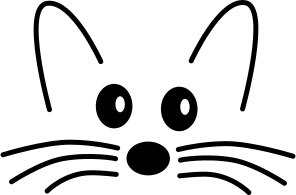
\includegraphics[width=1.4em]{squeak-logo}}}
\iftoshelse{
	\usepackage{marginnote}
		\renewcommand*{\marginfont}{\footnotesize}
	\newcommand{\vartriangleout}{\ifthenelse{\isodd{\thepage}}{\vartriangleright}{\vartriangleleft}}
	\newcommand{\dothisicon}{\fcolorbox{blue!65}{white}{\highlight{$\vartriangleout$}}}
	\newcommand{\dothis}[1]{%
		\noindent\par\noindent
		{\reversemarginpar
			\marginnote{\fcolorbox{blue!65}{white}{\highlight{$\vartriangleout$}}}}
		%\MarginLabel{do this}
		\noindent\emph{#1}
		\nopagebreak}
}{
	\newcommand{\dothisicon}{\raisebox{-.5ex}{
\includegraphics[height=1.2em]{pharo}}}
	\newcommand{\dothis}[1]{%
		\medskip
		\noindent\dothisicon
		\ifx#1\empty\else\quad\emph{#1}\fi
		\par\smallskip\nopagebreak}
}
%===> NEW VERSION <===
% NB: To use this in an individual chapter, you must set:
%\graphicspath{{figures/} {../figures/}}
% at the head of the chapter.  Don't forget the final /
%=============================================================
%:Reader hints (hint)
%
% Indicates a non-obvious consequence 
\newcommand{\hint}[1]{\vspace{1ex}\noindent\fbox{\textsc{Hint}} \emph{#1}}
%=================================================================
% graphics for Morphic handles
\newcommand{\grabHandle}{\raisebox{-0.2ex}{
\includegraphics[width=1em]{blackHandle}}}
\newcommand{\moveHandle}{\raisebox{-0.2ex}{
\includegraphics[width=1em]{moveHandle}}}
\newcommand{\debugHandle}{\raisebox{-0.2ex}{
\includegraphics[width=1em]{debugHandle}}}
%=============================================================
%:Highlighting Important stuff (doublebox)
%
% From Seaside book ...
\newsavebox{\SavedText}
\newlength{\InnerBoxRule}\setlength{\InnerBoxRule}{.75\fboxrule}
\newlength{\OuterBoxRule}\setlength{\OuterBoxRule}{1.5\fboxrule}
\newlength{\BoxSeparation}\setlength{\BoxSeparation}{1.5\fboxrule}
\addtolength{\BoxSeparation}{.5pt}
\newlength{\SaveBoxSep}\setlength{\SaveBoxSep}{2\fboxsep}
%
\newenvironment{doublebox}{\begin{lrbox}{\SavedText}
    \begin{minipage}{.75\textwidth}}
    {\end{minipage}\end{lrbox}\begin{center}
    \setlength{\fboxsep}{\BoxSeparation}\setlength{\fboxrule}{\OuterBoxRule}
    \fbox{\setlength{\fboxsep}{\SaveBoxSep}\setlength{\fboxrule}{\InnerBoxRule}%
      \fbox{\usebox{\SavedText}}}
  \end{center}}
% Use this:
\newcommand{\important}[1]{\begin{doublebox}#1\end{doublebox}}
%=============================================================
%:Section depth
\setcounter{secnumdepth}{2}
%% for this to happen start the file with
%\ifx\wholebook\relax\else
%% $Author$
% $Date$
% $Revision$

% HISTORY:
% 2006-10-31 - Oscar code macros
% ...

%=============================================================
% NB: documentclass must be set in main document.
% Allows book to be generated in multiple formats.
%=============================================================
%:Packages
\usepackage[T1]{fontenc}  %%%%%% really important to get the code directly in the text!
\usepackage{lmodern}
%\usepackage[scaled=0.85]{bookmanx} % needs another scale factor if used with \renewcommand{\sfdefault}{cmbr}
\usepackage{palatino}
\usepackage[scaled=0.85]{helvet}
\usepackage[protrusion,expansion=false]{microtype}
\usepackage{graphicx}
\usepackage{theorem}
\usepackage[english]{babel}
% ON: pdfsync breaks the use of p{width} for tabular columns!
\ifdefined\usepdfsync\usepackage{pdfsync}\fi % Requires texlive 2007
%=============================================================
%:More packages
%Stef should check which ones are used!
%\usepackage{picinpar}
%\usepackage{layout}
%\usepackage{color}
%\usepackage{enum}
%\usepackage{a4wide}
% \usepackage{fancyhdr}
\usepackage{ifthen}
\usepackage{float}
\usepackage{longtable}
\usepackage{makeidx}
\usepackage[nottoc]{tocbibind}
\usepackage{multicol}
\usepackage{booktabs}	% book-style tables
\usepackage{topcapt}	% enables \topcaption
\usepackage{multirow}
\usepackage{tabularx}
%\usepackage[bottom]{footmisc}
\usepackage{xspace}
\usepackage{alltt}
\usepackage{amssymb,textcomp}
\usepackage[usenames,dvipsnames]{color}
%\usepackage{colortbl}
\usepackage[hang]{subfigure}\makeatletter\def\p@subfigure{\thefigure\,}\makeatother
\usepackage{rotating}
\usepackage{enumitem}	% apb: allows more control over tags in enumerations
\usepackage{verbatim}     % for comment environment
\usepackage{varioref}	% for page references that work
\labelformat{footnote}{\thechapter--#1} % to distinguish citations from jurabib
\usepackage{needspace}
\usepackage{isodateo} % enable \isodate
\usepackage[newparttoc]{titlesec}
\usepackage{titletoc}
\usepackage{wrapfig}
\usepackage[
	super,
	citefull=first,
	authorformat={allreversed,and},
	titleformat={commasep,italic}
]{jurabib} % citations as footnotes
\usepackage[
	colorlinks=true,
	linkcolor=black,
	urlcolor=black,
	citecolor=black
]{hyperref}   % should come last
%=============================================================
%:PDF version
\pdfminorversion=3 % Set PDF to 1.3 for Lulu
%=============================================================
%:URL style
\makeatletter
\def\url@leostyle{%
  \@ifundefined{selectfont}{\def\UrlFont{\sf}}{\def\UrlFont{\sffamily}}}
\makeatother
% Now actually use the newly defined style.
\urlstyle{leo}
%=============================================================
%:Booleans
\newboolean{lulu}
\setboolean{lulu}{false}
\newcommand{\ifluluelse}[2]{\ifthenelse{\boolean{lulu}}{#1}{#2}}
%=============================================================
%:Names
\newcommand{\SUnit}{SUnit\xspace}
\newcommand{\sunit}{SUnit\xspace}
\newcommand{\xUnit}{$x$Unit\xspace}
\newcommand{\JUnit}{JUnit\xspace}
\newcommand{\st}{Smalltalk\xspace}
\newcommand{\pharo}{Pharo\xspace} % Use this, not \Pharo
%\newcommand{\sqmap}{SqueakMap\xspace}
\newcommand{\squeak}{Squeak\xspace} % use this, not \Squeak or \sq
\newcommand{\sqsrc}{SqueakSource\xspace}
\newcommand{\sbe}{\url{http://SqueakByExample.org}\xspace}
\newcommand{\pharoweb}{\url{http://pharo-project.org}\xspace}
\newcommand{\pbe}{\url{http://PharoByExample.org}\xspace}
\newcommand{\sba}{\url{http://SquareBracketAssociates.org}\xspace}
\newcommand{\bam}{\lct{Bounc\-ing\-Atoms\-Morph}\xspace}
%=============================================================
%:Markup macros for proof-reading
\usepackage[normalem]{ulem} % for \sout
\usepackage{xcolor}
\newcommand{\ra}{$\rightarrow$}
\newcommand{\ugh}[1]{\textcolor{red}{\uwave{#1}}} % please rephrase
\newcommand{\ins}[1]{\textcolor{blue}{\uline{#1}}} % please insert
\newcommand{\del}[1]{\textcolor{red}{\sout{#1}}} % please delete
\newcommand{\chg}[2]{\textcolor{red}{\sout{#1}}{\ra}\textcolor{blue}{\uline{#2}}} % please change
%=============================================================
%:Editorial comment macros
%\newcommand{\nnbb}[2]{
%    % \fbox{\bfseries\sffamily\scriptsize#1}
%    \fcolorbox{gray}{yellow}{\bfseries\sffamily\scriptsize#1}
%    {\sf\small$\blacktriangleright$\textit{#2}$\blacktriangleleft$}
%   }
\newcommand{\yellowbox}[1]{\fcolorbox{gray}{yellow}{\bfseries\sffamily\scriptsize#1}}
\newcommand{\triangles}[1]{{\sf\small$\blacktriangleright$\textit{#1}$\blacktriangleleft$}}
\newcommand{\nnbb}[2]{\yellowbox{#1} \triangles{#2}}
\newcommand{\fix}{\yellowbox{FIX!}}
\newcommand{\here}{\yellowbox{CONTINUE HERE!}}
% editor macros
\newcommand{\apl}[1]{\nnbb{Alain}{#1}} % Alain
\newcommand{\ab}[1]{\nnbb{Andrew}{#1}} % Black
\newcommand{\sd}[1]{\nnbb{St\'{e}f}{#1}} % Ducasse
\newcommand{\dc}[1]{\nnbb{DamienC}{#1}} % Ducasse
\newcommand{\md}[1]{\nnbb{Marcus}{#1}} % Denker
\newcommand{\on}[1]{\nnbb{Oscar}{#1}} % Nierstrasz
\newcommand{\damien}[1]{\nnbb{Damien}{#1}} % Pollet
\newcommand{\lr}[1]{\nnbb{Lukas}{#1}} % Renggli
\newcommand{\orla}[1]{\nnbb{Orla}{#1}} % Greevy
\newcommand{\alex}[1]{\nnbb{Alex}{#1}} % Bergel
\newcommand{\alx}[1]{\nnbb{Alex}{#1}} % Bergel
\newcommand{\dr}[1]{\nnbb{David}{#1}} % Roethlisberger
\newcommand{\ja}[1]{\nnbb{Jannik}{#1}} % Laval
\newcommand{\jr}[1]{\nnbb{Jorge}{#1}} % Ressia
\newcommand{\jb}[1]{\nnbb{JB}{#1}} % JB
\newcommand{\fp}[1]{\nnbb{Fabrizio}{#1}} % Perin
\newcommand{\michael}[1]{\nnbb{Michael}{#1}} % Davies
\newcommand{\ew}[1]{\nnbb{Erwann}{#1}} % Wernli
\newcommand{\mb}[1]{\nnbb{Martial}{#1}} % Boniou
\newcommand{\hw}[1]{\nnbb{Hernan}{#1}} % Wilkinson
\newcommand{\ben}[1]{\nnbb{Benjamin}{#1}} % Benjamin Van Ryseghem
%=============================================================
%:Abbreviation macros
\newcommand{\ie}{\emph{i.e.},\xspace}
\newcommand{\eg}{\emph{e.g.},\xspace}
\newcommand{\etc}{etc.\xspace}
%=============================================================
%:Cross reference macros
\newcommand{\charef}[1]{Chapter~\ref{cha:#1}\xspace}
\newcommand{\secref}[1]{Section~\ref{sec:#1}\xspace}
\newcommand{\figref}[1]{Figure~\ref{fig:#1}\xspace}
\newcommand{\Figref}[1]{Figure~\ref{fig:#1}\xspace}
\newcommand{\appref}[1]{Appendix~\ref{app:#1}\xspace}
\newcommand{\tabref}[1]{Table~\ref{tab:#1}\xspace}
\newcommand{\faqref}[1]{FAQ~\ref{faq:#1}, p.~\pageref{faq:#1}\xspace}
% APB: I removed trailing \xspace commands from these macros because
% \xspace mostly doesn't work.  If you want a space after your
% references, type one!
% ON: xspace has always worked just fine for me!  Please leave them in.
%
\newcommand{\ruleref}[1]{\ref{rule:#1}\xspace}
%
\newcommand{\egref}[1]{example~\ref{eg:#1}\xspace}
\newcommand{\Egref}[1]{Example~\ref{eg:#1}\xspace}
%
\newcommand{\scrref}[1]{script~\ref{scr:#1}\xspace}
\newcommand{\Scrref}[1]{Script~\ref{scr:#1}\xspace}
\newcommand{\tscrref}[1]{the script~\ref{scr:#1}\xspace}
\newcommand{\Tscrref}[1]{The script~\ref{scr:#1}\xspace}
%
\newcommand{\mthref}[1]{method~\ref{mth:#1}\xspace}
\newcommand{\mthsref}[1]{methods~\ref{mth:#1}\xspace}
\newcommand{\Mthref}[1]{Method~\ref{mth:#1}\xspace}
\newcommand{\tmthref}[1]{the method~\ref{mth:#1}\xspace}
\newcommand{\Tmthref}[1]{The method~\ref{mth:#1}\xspace}
%
\newcommand{\clsref}[1]{class~\ref{cls:#1}\xspace}
\newcommand{\tclsref}[1]{the class~\ref{cls:#1}\xspace}
\newcommand{\Tclsref}[1]{The class~\ref{cls:#1}\xspace}

\newcommand{\chalabel}[1]{\label{cha:#1}}
\newcommand{\seclabel}[1]{\label{sec:#1}}
\newcommand{\figlabel}[1]{\label{fig:#1}}
\newcommand{\tablabel}[1]{\label{tab:#1}}
\newcommand{\rulelabel}[1]{\label{rule:#1}}
\newcommand{\eglabel}[1]{\label{eg:#1}}
\newcommand{\scrlabel}[1]{\label{scr:#1}}
\newcommand{\mthlabel}[1]{\label{mth:#1}}
\newcommand{\clslabel}[1]{\label{cls:#1}}
\newcommand{\faqlabel}[1]{\label{faq:#1}}
%=============================================================
%:Menu item macro
% for menu items, so we can change our minds on how to print them! (apb)
\definecolor{lightgray}{gray}{0.89}
\newcommand{\menu}[1]{{%
	\setlength{\fboxsep}{0pt}%
	\colorbox{lightgray}{{{\upshape\sffamily\strut \,#1\,}}}}}
\newcommand{\link}[1]{{%
	\fontfamily{lmr}\selectfont
 	\upshape{\sffamily \underline{#1}}}}
% For submenu items:
\newcommand{\go}{\,$\triangleright$\,}
% \newcommand{\go}{\,$\blacktriangleright$\,}
% For keyboard shortcuts:
%\newcommand{\short}[1]{\mbox{$\langle${\sc CMD}$\rangle$-#1}\xspace}
\newcommand{\short}[1]{\mbox{{\sc cmd}\hspace{0.08em}--\hspace{0.09em}#1}\xspace}
% For buttons:
\newcommand{\button}[1]{{%
	\setlength{\fboxsep}{0pt}%
	\fbox{{\upshape\sffamily\strut \,#1\,}}}}
% NB: The button macro does not work within captions -- incompatible with xcolor package :-(
\newcommand{\toolsflap}{\textit{Tools} flap\xspace}
%=============================================================
%:Mouse clicks
\newcommand{\click}{click\xspace} % RED
\newcommand{\actclick}{action-click\xspace} % YELLOW
\newcommand{\metaclick}{meta-click\xspace} % BLUE
\newcommand{\Click}{Click\xspace} % RED
\newcommand{\Actclick}{Action-click\xspace} % YELLOW
\newcommand{\Metaclick}{Meta-click\xspace} % BLUE
%=============================================================
%:ToSh macros
\newboolean{tosh}
\setboolean{tosh}{false}
\newcommand{\iftoshelse}[2]{\ifthenelse{\boolean{tosh}}{#1}{#2}}
%=============================================================
%:ToSh colors
%\newcommand{\highlightcolor}{\color{blue!65}}
%\newcommand{\boxcolor}{\color{gray!25}}
\newcommand{\highlight}[1]{\textcolor{blue!65}{#1}}
%\newcommand{\codecolor}{\color{blue!65}}
%%\setlength{\fboxrule}{2pt}
%\newcommand{\asPict}[1]{%
%	{\Large\highlight{#1}}}
%=============================================================
%:Reader cues (do this)
%
% Indicate something the reader should try out.
% \newcommand{\dothisicon}{\raisebox{-.5ex}{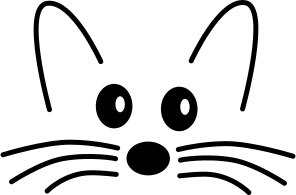
\includegraphics[width=1.4em]{squeak-logo}}}
\iftoshelse{
	\usepackage{marginnote}
		\renewcommand*{\marginfont}{\footnotesize}
	\newcommand{\vartriangleout}{\ifthenelse{\isodd{\thepage}}{\vartriangleright}{\vartriangleleft}}
	\newcommand{\dothisicon}{\fcolorbox{blue!65}{white}{\highlight{$\vartriangleout$}}}
	\newcommand{\dothis}[1]{%
		\noindent\par\noindent
		{\reversemarginpar
			\marginnote{\fcolorbox{blue!65}{white}{\highlight{$\vartriangleout$}}}}
		%\MarginLabel{do this}
		\noindent\emph{#1}
		\nopagebreak}
}{
	\newcommand{\dothisicon}{\raisebox{-.5ex}{
\includegraphics[height=1.2em]{pharo}}}
	\newcommand{\dothis}[1]{%
		\medskip
		\noindent\dothisicon
		\ifx#1\empty\else\quad\emph{#1}\fi
		\par\smallskip\nopagebreak}
}
%===> NEW VERSION <===
% NB: To use this in an individual chapter, you must set:
%\graphicspath{{figures/} {../figures/}}
% at the head of the chapter.  Don't forget the final /
%=============================================================
%:Reader hints (hint)
%
% Indicates a non-obvious consequence 
\newcommand{\hint}[1]{\vspace{1ex}\noindent\fbox{\textsc{Hint}} \emph{#1}}
%=================================================================
% graphics for Morphic handles
\newcommand{\grabHandle}{\raisebox{-0.2ex}{
\includegraphics[width=1em]{blackHandle}}}
\newcommand{\moveHandle}{\raisebox{-0.2ex}{
\includegraphics[width=1em]{moveHandle}}}
\newcommand{\debugHandle}{\raisebox{-0.2ex}{
\includegraphics[width=1em]{debugHandle}}}
%=============================================================
%:Highlighting Important stuff (doublebox)
%
% From Seaside book ...
\newsavebox{\SavedText}
\newlength{\InnerBoxRule}\setlength{\InnerBoxRule}{.75\fboxrule}
\newlength{\OuterBoxRule}\setlength{\OuterBoxRule}{1.5\fboxrule}
\newlength{\BoxSeparation}\setlength{\BoxSeparation}{1.5\fboxrule}
\addtolength{\BoxSeparation}{.5pt}
\newlength{\SaveBoxSep}\setlength{\SaveBoxSep}{2\fboxsep}
%
\newenvironment{doublebox}{\begin{lrbox}{\SavedText}
    \begin{minipage}{.75\textwidth}}
    {\end{minipage}\end{lrbox}\begin{center}
    \setlength{\fboxsep}{\BoxSeparation}\setlength{\fboxrule}{\OuterBoxRule}
    \fbox{\setlength{\fboxsep}{\SaveBoxSep}\setlength{\fboxrule}{\InnerBoxRule}%
      \fbox{\usebox{\SavedText}}}
  \end{center}}
% Use this:
\newcommand{\important}[1]{\begin{doublebox}#1\end{doublebox}}
%=============================================================
%:Section depth
\setcounter{secnumdepth}{2}
%% for this to happen start the file with
%\ifx\wholebook\relax\else
%% $Author$
% $Date$
% $Revision$

% HISTORY:
% 2006-10-31 - Oscar code macros
% ...

%=============================================================
% NB: documentclass must be set in main document.
% Allows book to be generated in multiple formats.
%=============================================================
%:Packages
\usepackage[T1]{fontenc}  %%%%%% really important to get the code directly in the text!
\usepackage{lmodern}
%\usepackage[scaled=0.85]{bookmanx} % needs another scale factor if used with \renewcommand{\sfdefault}{cmbr}
\usepackage{palatino}
\usepackage[scaled=0.85]{helvet}
\usepackage[protrusion,expansion=false]{microtype}
\usepackage{graphicx}
\usepackage{theorem}
\usepackage[english]{babel}
% ON: pdfsync breaks the use of p{width} for tabular columns!
\ifdefined\usepdfsync\usepackage{pdfsync}\fi % Requires texlive 2007
%=============================================================
%:More packages
%Stef should check which ones are used!
%\usepackage{picinpar}
%\usepackage{layout}
%\usepackage{color}
%\usepackage{enum}
%\usepackage{a4wide}
% \usepackage{fancyhdr}
\usepackage{ifthen}
\usepackage{float}
\usepackage{longtable}
\usepackage{makeidx}
\usepackage[nottoc]{tocbibind}
\usepackage{multicol}
\usepackage{booktabs}	% book-style tables
\usepackage{topcapt}	% enables \topcaption
\usepackage{multirow}
\usepackage{tabularx}
%\usepackage[bottom]{footmisc}
\usepackage{xspace}
\usepackage{alltt}
\usepackage{amssymb,textcomp}
\usepackage[usenames,dvipsnames]{color}
%\usepackage{colortbl}
\usepackage[hang]{subfigure}\makeatletter\def\p@subfigure{\thefigure\,}\makeatother
\usepackage{rotating}
\usepackage{enumitem}	% apb: allows more control over tags in enumerations
\usepackage{verbatim}     % for comment environment
\usepackage{varioref}	% for page references that work
\labelformat{footnote}{\thechapter--#1} % to distinguish citations from jurabib
\usepackage{needspace}
\usepackage{isodateo} % enable \isodate
\usepackage[newparttoc]{titlesec}
\usepackage{titletoc}
\usepackage{wrapfig}
\usepackage[
	super,
	citefull=first,
	authorformat={allreversed,and},
	titleformat={commasep,italic}
]{jurabib} % citations as footnotes
\usepackage[
	colorlinks=true,
	linkcolor=black,
	urlcolor=black,
	citecolor=black
]{hyperref}   % should come last
%=============================================================
%:PDF version
\pdfminorversion=3 % Set PDF to 1.3 for Lulu
%=============================================================
%:URL style
\makeatletter
\def\url@leostyle{%
  \@ifundefined{selectfont}{\def\UrlFont{\sf}}{\def\UrlFont{\sffamily}}}
\makeatother
% Now actually use the newly defined style.
\urlstyle{leo}
%=============================================================
%:Booleans
\newboolean{lulu}
\setboolean{lulu}{false}
\newcommand{\ifluluelse}[2]{\ifthenelse{\boolean{lulu}}{#1}{#2}}
%=============================================================
%:Names
\newcommand{\SUnit}{SUnit\xspace}
\newcommand{\sunit}{SUnit\xspace}
\newcommand{\xUnit}{$x$Unit\xspace}
\newcommand{\JUnit}{JUnit\xspace}
\newcommand{\st}{Smalltalk\xspace}
\newcommand{\pharo}{Pharo\xspace} % Use this, not \Pharo
%\newcommand{\sqmap}{SqueakMap\xspace}
\newcommand{\squeak}{Squeak\xspace} % use this, not \Squeak or \sq
\newcommand{\sqsrc}{SqueakSource\xspace}
\newcommand{\sbe}{\url{http://SqueakByExample.org}\xspace}
\newcommand{\pharoweb}{\url{http://pharo-project.org}\xspace}
\newcommand{\pbe}{\url{http://PharoByExample.org}\xspace}
\newcommand{\sba}{\url{http://SquareBracketAssociates.org}\xspace}
\newcommand{\bam}{\lct{Bounc\-ing\-Atoms\-Morph}\xspace}
%=============================================================
%:Markup macros for proof-reading
\usepackage[normalem]{ulem} % for \sout
\usepackage{xcolor}
\newcommand{\ra}{$\rightarrow$}
\newcommand{\ugh}[1]{\textcolor{red}{\uwave{#1}}} % please rephrase
\newcommand{\ins}[1]{\textcolor{blue}{\uline{#1}}} % please insert
\newcommand{\del}[1]{\textcolor{red}{\sout{#1}}} % please delete
\newcommand{\chg}[2]{\textcolor{red}{\sout{#1}}{\ra}\textcolor{blue}{\uline{#2}}} % please change
%=============================================================
%:Editorial comment macros
%\newcommand{\nnbb}[2]{
%    % \fbox{\bfseries\sffamily\scriptsize#1}
%    \fcolorbox{gray}{yellow}{\bfseries\sffamily\scriptsize#1}
%    {\sf\small$\blacktriangleright$\textit{#2}$\blacktriangleleft$}
%   }
\newcommand{\yellowbox}[1]{\fcolorbox{gray}{yellow}{\bfseries\sffamily\scriptsize#1}}
\newcommand{\triangles}[1]{{\sf\small$\blacktriangleright$\textit{#1}$\blacktriangleleft$}}
\newcommand{\nnbb}[2]{\yellowbox{#1} \triangles{#2}}
\newcommand{\fix}{\yellowbox{FIX!}}
\newcommand{\here}{\yellowbox{CONTINUE HERE!}}
% editor macros
\newcommand{\apl}[1]{\nnbb{Alain}{#1}} % Alain
\newcommand{\ab}[1]{\nnbb{Andrew}{#1}} % Black
\newcommand{\sd}[1]{\nnbb{St\'{e}f}{#1}} % Ducasse
\newcommand{\dc}[1]{\nnbb{DamienC}{#1}} % Ducasse
\newcommand{\md}[1]{\nnbb{Marcus}{#1}} % Denker
\newcommand{\on}[1]{\nnbb{Oscar}{#1}} % Nierstrasz
\newcommand{\damien}[1]{\nnbb{Damien}{#1}} % Pollet
\newcommand{\lr}[1]{\nnbb{Lukas}{#1}} % Renggli
\newcommand{\orla}[1]{\nnbb{Orla}{#1}} % Greevy
\newcommand{\alex}[1]{\nnbb{Alex}{#1}} % Bergel
\newcommand{\alx}[1]{\nnbb{Alex}{#1}} % Bergel
\newcommand{\dr}[1]{\nnbb{David}{#1}} % Roethlisberger
\newcommand{\ja}[1]{\nnbb{Jannik}{#1}} % Laval
\newcommand{\jr}[1]{\nnbb{Jorge}{#1}} % Ressia
\newcommand{\jb}[1]{\nnbb{JB}{#1}} % JB
\newcommand{\fp}[1]{\nnbb{Fabrizio}{#1}} % Perin
\newcommand{\michael}[1]{\nnbb{Michael}{#1}} % Davies
\newcommand{\ew}[1]{\nnbb{Erwann}{#1}} % Wernli
\newcommand{\mb}[1]{\nnbb{Martial}{#1}} % Boniou
\newcommand{\hw}[1]{\nnbb{Hernan}{#1}} % Wilkinson
\newcommand{\ben}[1]{\nnbb{Benjamin}{#1}} % Benjamin Van Ryseghem
%=============================================================
%:Abbreviation macros
\newcommand{\ie}{\emph{i.e.},\xspace}
\newcommand{\eg}{\emph{e.g.},\xspace}
\newcommand{\etc}{etc.\xspace}
%=============================================================
%:Cross reference macros
\newcommand{\charef}[1]{Chapter~\ref{cha:#1}\xspace}
\newcommand{\secref}[1]{Section~\ref{sec:#1}\xspace}
\newcommand{\figref}[1]{Figure~\ref{fig:#1}\xspace}
\newcommand{\Figref}[1]{Figure~\ref{fig:#1}\xspace}
\newcommand{\appref}[1]{Appendix~\ref{app:#1}\xspace}
\newcommand{\tabref}[1]{Table~\ref{tab:#1}\xspace}
\newcommand{\faqref}[1]{FAQ~\ref{faq:#1}, p.~\pageref{faq:#1}\xspace}
% APB: I removed trailing \xspace commands from these macros because
% \xspace mostly doesn't work.  If you want a space after your
% references, type one!
% ON: xspace has always worked just fine for me!  Please leave them in.
%
\newcommand{\ruleref}[1]{\ref{rule:#1}\xspace}
%
\newcommand{\egref}[1]{example~\ref{eg:#1}\xspace}
\newcommand{\Egref}[1]{Example~\ref{eg:#1}\xspace}
%
\newcommand{\scrref}[1]{script~\ref{scr:#1}\xspace}
\newcommand{\Scrref}[1]{Script~\ref{scr:#1}\xspace}
\newcommand{\tscrref}[1]{the script~\ref{scr:#1}\xspace}
\newcommand{\Tscrref}[1]{The script~\ref{scr:#1}\xspace}
%
\newcommand{\mthref}[1]{method~\ref{mth:#1}\xspace}
\newcommand{\mthsref}[1]{methods~\ref{mth:#1}\xspace}
\newcommand{\Mthref}[1]{Method~\ref{mth:#1}\xspace}
\newcommand{\tmthref}[1]{the method~\ref{mth:#1}\xspace}
\newcommand{\Tmthref}[1]{The method~\ref{mth:#1}\xspace}
%
\newcommand{\clsref}[1]{class~\ref{cls:#1}\xspace}
\newcommand{\tclsref}[1]{the class~\ref{cls:#1}\xspace}
\newcommand{\Tclsref}[1]{The class~\ref{cls:#1}\xspace}

\newcommand{\chalabel}[1]{\label{cha:#1}}
\newcommand{\seclabel}[1]{\label{sec:#1}}
\newcommand{\figlabel}[1]{\label{fig:#1}}
\newcommand{\tablabel}[1]{\label{tab:#1}}
\newcommand{\rulelabel}[1]{\label{rule:#1}}
\newcommand{\eglabel}[1]{\label{eg:#1}}
\newcommand{\scrlabel}[1]{\label{scr:#1}}
\newcommand{\mthlabel}[1]{\label{mth:#1}}
\newcommand{\clslabel}[1]{\label{cls:#1}}
\newcommand{\faqlabel}[1]{\label{faq:#1}}
%=============================================================
%:Menu item macro
% for menu items, so we can change our minds on how to print them! (apb)
\definecolor{lightgray}{gray}{0.89}
\newcommand{\menu}[1]{{%
	\setlength{\fboxsep}{0pt}%
	\colorbox{lightgray}{{{\upshape\sffamily\strut \,#1\,}}}}}
\newcommand{\link}[1]{{%
	\fontfamily{lmr}\selectfont
 	\upshape{\sffamily \underline{#1}}}}
% For submenu items:
\newcommand{\go}{\,$\triangleright$\,}
% \newcommand{\go}{\,$\blacktriangleright$\,}
% For keyboard shortcuts:
%\newcommand{\short}[1]{\mbox{$\langle${\sc CMD}$\rangle$-#1}\xspace}
\newcommand{\short}[1]{\mbox{{\sc cmd}\hspace{0.08em}--\hspace{0.09em}#1}\xspace}
% For buttons:
\newcommand{\button}[1]{{%
	\setlength{\fboxsep}{0pt}%
	\fbox{{\upshape\sffamily\strut \,#1\,}}}}
% NB: The button macro does not work within captions -- incompatible with xcolor package :-(
\newcommand{\toolsflap}{\textit{Tools} flap\xspace}
%=============================================================
%:Mouse clicks
\newcommand{\click}{click\xspace} % RED
\newcommand{\actclick}{action-click\xspace} % YELLOW
\newcommand{\metaclick}{meta-click\xspace} % BLUE
\newcommand{\Click}{Click\xspace} % RED
\newcommand{\Actclick}{Action-click\xspace} % YELLOW
\newcommand{\Metaclick}{Meta-click\xspace} % BLUE
%=============================================================
%:ToSh macros
\newboolean{tosh}
\setboolean{tosh}{false}
\newcommand{\iftoshelse}[2]{\ifthenelse{\boolean{tosh}}{#1}{#2}}
%=============================================================
%:ToSh colors
%\newcommand{\highlightcolor}{\color{blue!65}}
%\newcommand{\boxcolor}{\color{gray!25}}
\newcommand{\highlight}[1]{\textcolor{blue!65}{#1}}
%\newcommand{\codecolor}{\color{blue!65}}
%%\setlength{\fboxrule}{2pt}
%\newcommand{\asPict}[1]{%
%	{\Large\highlight{#1}}}
%=============================================================
%:Reader cues (do this)
%
% Indicate something the reader should try out.
% \newcommand{\dothisicon}{\raisebox{-.5ex}{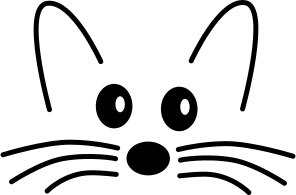
\includegraphics[width=1.4em]{squeak-logo}}}
\iftoshelse{
	\usepackage{marginnote}
		\renewcommand*{\marginfont}{\footnotesize}
	\newcommand{\vartriangleout}{\ifthenelse{\isodd{\thepage}}{\vartriangleright}{\vartriangleleft}}
	\newcommand{\dothisicon}{\fcolorbox{blue!65}{white}{\highlight{$\vartriangleout$}}}
	\newcommand{\dothis}[1]{%
		\noindent\par\noindent
		{\reversemarginpar
			\marginnote{\fcolorbox{blue!65}{white}{\highlight{$\vartriangleout$}}}}
		%\MarginLabel{do this}
		\noindent\emph{#1}
		\nopagebreak}
}{
	\newcommand{\dothisicon}{\raisebox{-.5ex}{
\includegraphics[height=1.2em]{pharo}}}
	\newcommand{\dothis}[1]{%
		\medskip
		\noindent\dothisicon
		\ifx#1\empty\else\quad\emph{#1}\fi
		\par\smallskip\nopagebreak}
}
%===> NEW VERSION <===
% NB: To use this in an individual chapter, you must set:
%\graphicspath{{figures/} {../figures/}}
% at the head of the chapter.  Don't forget the final /
%=============================================================
%:Reader hints (hint)
%
% Indicates a non-obvious consequence 
\newcommand{\hint}[1]{\vspace{1ex}\noindent\fbox{\textsc{Hint}} \emph{#1}}
%=================================================================
% graphics for Morphic handles
\newcommand{\grabHandle}{\raisebox{-0.2ex}{
\includegraphics[width=1em]{blackHandle}}}
\newcommand{\moveHandle}{\raisebox{-0.2ex}{
\includegraphics[width=1em]{moveHandle}}}
\newcommand{\debugHandle}{\raisebox{-0.2ex}{
\includegraphics[width=1em]{debugHandle}}}
%=============================================================
%:Highlighting Important stuff (doublebox)
%
% From Seaside book ...
\newsavebox{\SavedText}
\newlength{\InnerBoxRule}\setlength{\InnerBoxRule}{.75\fboxrule}
\newlength{\OuterBoxRule}\setlength{\OuterBoxRule}{1.5\fboxrule}
\newlength{\BoxSeparation}\setlength{\BoxSeparation}{1.5\fboxrule}
\addtolength{\BoxSeparation}{.5pt}
\newlength{\SaveBoxSep}\setlength{\SaveBoxSep}{2\fboxsep}
%
\newenvironment{doublebox}{\begin{lrbox}{\SavedText}
    \begin{minipage}{.75\textwidth}}
    {\end{minipage}\end{lrbox}\begin{center}
    \setlength{\fboxsep}{\BoxSeparation}\setlength{\fboxrule}{\OuterBoxRule}
    \fbox{\setlength{\fboxsep}{\SaveBoxSep}\setlength{\fboxrule}{\InnerBoxRule}%
      \fbox{\usebox{\SavedText}}}
  \end{center}}
% Use this:
\newcommand{\important}[1]{\begin{doublebox}#1\end{doublebox}}
%=============================================================
%:Section depth
\setcounter{secnumdepth}{2}
%% for this to happen start the file with
%\ifx\wholebook\relax\else
%\input{../common.tex}
%\begin{document}
%\fi
% and terminate by
% \ifx\wholebook\relax\else\end{document}\fi

\DeclareGraphicsExtensions{.pdf, .jpg, .png}
%=============================================================
%:PDF setup
\hypersetup{
%   a4paper,
%   pdfstartview=FitV,
%   colorlinks,
%   linkcolor=darkblue,
%   citecolor=darkblue,
   pdftitle={Pharo by Example},
   pdfauthor={Andrew P. Black, St\'ephane Ducasse,	Oscar Nierstrasz,
Damien Pollet},
   pdfkeywords={Smalltalk, Squeak, Object-Oriented Programming, OOP},
   pdfsubject={Computer Science}
}
%=============================================================
%:Page layout and appearance
%
% \renewcommand{\headrulewidth}{0pt}
\renewcommand{\chaptermark}[1]{\markboth{#1}{}}
\renewcommand{\sectionmark}[1]{\markright{\thesection\ #1}}
\renewpagestyle{plain}[\small\itshape]{%
	\setheadrule{0pt}%
	\sethead[][][]{}{}{}%
	\setfoot[][][]{}{}{}}
\renewpagestyle{headings}[\small\itshape]{%
	\setheadrule{0pt}%
	\setmarks{chapter}{section}%
	\sethead[\thepage][][\chaptertitle]{\sectiontitle}{}{\thepage}%
	\setfoot[][][]{}{}{}}
%=============================================================
%:Title section setup and TOC numbering depth
\setcounter{secnumdepth}{1}
\setcounter{tocdepth}{1}
\titleformat{\part}[display]{\centering}{\huge\partname\ \thepart}{1em}{\Huge\textbf}[]
\titleformat{\chapter}[display]{}{\huge\chaptertitlename\ \thechapter}{1em}{\Huge\raggedright\textbf}[]
\titlecontents{part}[3pc]{%
		\pagebreak[2]\addvspace{1em plus.4em minus.2em}%
		\leavevmode\large\bfseries}
	{\contentslabel{3pc}}{\hspace*{-3pc}}
	{}[\nopagebreak]
\titlecontents{chapter}[3pc]{%
		\pagebreak[0]\addvspace{1em plus.2em minus.2em}%
		\leavevmode\bfseries}
	{\contentslabel{3pc}}{}
	{\hfill\contentspage}[\nopagebreak]
\dottedcontents{section}[3pc]{}{3pc}{1pc}
\dottedcontents{subsection}[3pc]{}{0pc}{1pc}
% \dottedcontents{subsection}[4.5em]{}{0pt}{1pc}
% Make \cleardoublepage insert really blank pages http://www.tex.ac.uk/cgi-bin/texfaq2html?label=reallyblank
\let\origdoublepage\cleardoublepage
\newcommand{\clearemptydoublepage}{%
  \clearpage
  {\pagestyle{empty}\origdoublepage}}
\let\cleardoublepage\clearemptydoublepage % see http://www.tex.ac.uk/cgi-bin/texfaq2html?label=patch
%=============================================================
%:FAQ macros (for FAQ chapter)
\newtheorem{faq}{FAQ}
\newcommand{\answer}{\paragraph{Answer}\ }
%=============================================================
%:Listings package configuration
% \newcommand{\caret}{\makebox{\raisebox{0.4ex}{\footnotesize{$\wedge$}}}}
\newcommand{\caret}{\^\,}
\newcommand{\escape}{{\sf \textbackslash}}
\definecolor{source}{gray}{0.95}
\usepackage{listings}
\lstdefinelanguage{Smalltalk}{
%  morekeywords={self,super,true,false,nil,thisContext}, % This is overkill
  morestring=[d]',
  morecomment=[s]{"}{"},
  alsoletter={\#:},
  escapechar={!},
  literate=
    {BANG}{!}1
    {CARET}{\^}1
    {UNDERSCORE}{\_}1
    {\\st}{Smalltalk}9 % convenience -- in case \st occurs in code
    % {'}{{\textquotesingle}}1 % replaced by upquote=true in \lstset
    {_}{{$\leftarrow$}}1
    {>>>}{{\sep}}1
    {^}{{$\uparrow$}}1
    {~}{{$\sim$}}1
    {-}{{\texttt{-}}}1 %{\textminus}}1 %{-}{\hspace{-0.13em}}{-}}1  % the goal is to make - the same width as +
    % {+}{\sf+}1 %{\raisebox{0.08ex}{+}}}1      % and to raise + off the baseline to match -
    {-->}{{\quad$\longrightarrow$\quad}}3
	, % Don't forget the comma at the end!
  tabsize=4
}[keywords,comments,strings]

\lstset{language=Smalltalk,
	basicstyle=\sffamily,
	keywordstyle=\color{black}\bfseries,
	% stringstyle=\ttfamily, % Ugly! do we really want this? -- on
	mathescape=true,
	showstringspaces=false,
	keepspaces=true,
	breaklines=true,
	breakautoindent=true,
	backgroundcolor=\color{source},
	lineskip={-1pt}, % Ugly hack
	upquote=true, % straight quote; requires textcomp package
	columns=fullflexible} % no fixed width fonts
% In-line code (literal)
% Normally use this for all in-line code:
\newcommand{\ct}{\lstinline[mathescape=false,backgroundcolor=\color{white},basicstyle={\sffamily\upshape}]}
% apb 2007.8.28 added the \upshape declaration to avoid getting italicized code in \dothis{ } sections.
% In-line code (latex enabled)
% Use this only in special situations where \ct does not work
% (within section headings ...):
\newcommand{\lct}[1]{{\textsf{\textup{#1}}}}
% Use these for system categories and protocols:
\newcommand{\scat}[1]{\emph{\textsf{#1}}\xspace}
\newcommand{\pkg}[1]{\emph{\textsf{#1}}\xspace}
\newcommand{\prot}[1]{\emph{\textsf{#1}}\xspace}
% Code environments
% NB: the arg is for tests
% Only code and example environments may be tests
\lstnewenvironment{code}[1]{%
	\lstset{%
		% frame=lines,
		frame=single,
		framerule=0pt,
		mathescape=false
	}
}{}
\def\ignoredollar#1{}
%=============================================================
%:Code environments (method, script ...)
% NB: the third arg is for tests
% Only code and example environments may be tests
\lstnewenvironment{example}[3][defaultlabel]{%
	\renewcommand{\lstlistingname}{Example}%
	\lstset{
		% frame=lines,
		frame=single,
		framerule=0pt,
		mathescape=false,
		caption={\emph{#2}},
		label={eg:#1}
	}
}{}
\lstnewenvironment{script}[2][defaultlabel]{%
\renewcommand{\lstlistingname}{Script}%
	\lstset{
		% frame=lines,
		frame=single,
		framerule=0pt,
		mathescape=false,
		name={Script},
		caption={\emph{#2}},
		label={scr:#1}
	}
}{}
\lstnewenvironment{method}[2][defaultlabel]{%
	\renewcommand{\lstlistingname}{Method}%
	\lstset{
		% frame=lines,
		frame=single,
		framerule=0pt,
		mathescape=false,
		name={Method},
		caption={\emph{#2}},
		label={mth:#1}
	}
}{}
\lstnewenvironment{methods}[2][defaultlabel]{% just for multiple methods at once
	\renewcommand{\lstlistingname}{Methods}%
	\lstset{
		% frame=lines,
		frame=single,
		framerule=0pt,
		mathescape=false,
		name={Method},
		caption={\emph{#2}},
		label={mth:#1}
	}
}{}
\lstnewenvironment{numMethod}[2][defaultlabel]{%
	\renewcommand{\lstlistingname}{Method}%
	\lstset{
		numbers=left,
		numberstyle={\tiny\sffamily},
		% frame=lines,
		frame=single,
		framerule=0pt,
		mathescape=false,
		name={Method},
		caption={\emph{#2}},
		label={mth:#1}
	}
}{}
\lstnewenvironment{classdef}[2][defaultlabel]{%
	\renewcommand{\lstlistingname}{Class}%
	\lstset{
		% frame=lines,
		frame=single,
		framerule=0pt,
		mathescape=false,
		name={Class},
		caption={\emph{#2}},
		label={cls:#1}
	}
}{}
%=============================================================
%:Reserving space
% Usually need one more line than the actual lines of code
\newcommand{\needlines}[1]{\Needspace{#1\baselineskip}}
%=============================================================
%:Indexing macros
% Macros ending with "ind" generate text as well as an index entry
% Macros ending with "index" *only* generate an index entry
\newcommand{\ind}[1]{\index{#1}#1\xspace} % plain text
\newcommand{\subind}[2]{\index{#1!#2}#2\xspace} % show #2, subindex under #1
\newcommand{\emphind}[1]{\index{#1}\emph{#1}\xspace} % emph #1
\newcommand{\emphsubind}[2]{\index{#1!#2}\emph{#2}\xspace} % show emph #2, subindex inder #1
\newcommand{\scatind}[1]{\index{#1@\textsf{#1} (category)}\scat{#1}} % category
\newcommand{\pkgind}[1]{\index{#1@\textsf{#1} (package)}\pkg{#1}} % package
\newcommand{\protind}[1]{\index{#1@\textsf{#1} (protocol)}\prot{#1}} % protocol
\newcommand{\clsind}[1]{\index{#1@\textsf{#1} (class)}\ct{#1}\xspace}
% \newcommand{\clsind}[1]{\index{#1!\#@(class)}\ct{#1}\xspace} % class
\newcommand{\clsindplural}[1]{\index{#1!\#@(class)}\ct{#1}s\xspace} % class
\newcommand{\cvind}[1]{\index{#1@\textsf{#1} (class variable)}\ct{#1}\xspace} % class var
\newcommand{\glbind}[1]{\index{#1@\textsf{#1} (global)}\ct{#1}\xspace} % global
\newcommand{\patind}[1]{\index{#1@#1 (pattern)}\ct{#1}\xspace} % pattern
\newcommand{\pvind}[1]{\index{#1@\textsf{#1} (pseudo variable)}\ct{#1}\xspace} % pseudo var
\newcommand{\clsmthind}[2]{\index{#1!#2@\ct{#2}}\ct{#1>>>#2}\xspace} % class + method name
\newcommand{\mthind}[2]{\index{#1!#2@\ct{#2}}\ct{#2}\xspace} % show method name only
\newcommand{\lmthind}[2]{\index{#1!#2@\ct{#2}}\lct{#2}\xspace} % show method name only
\newcommand{\cmind}[2]{\index{#1!#2@\ct{#2}}\ct{#1>>>#2}\xspace} % show class>>method
\newcommand{\lcmind}[2]{\index{#1!#2@\ct{#2}}\lct{#1>>>#2}\xspace} % show class>>method
\newcommand{\toolsflapind}{\index{Tools flap}\toolsflap} % index tools flap
% The following only generate an index entry:
% \newcommand{\clsindex}[1]{\index{#1@\textsf{#1} (class)}}
\newcommand{\clsindex}[1]{\index{#1!\#@(class)}} % class
\newcommand{\mthindex}[2]{\index{#1!#2@\ct{#2}}} % method
\newcommand{\cmindex}[2]{\index{#1!#2@\ct{#2}}} % class>>method
\newcommand{\cvindex}[1]{\index{#1@\textsf{#1} (class variable)}} % class var
\newcommand{\glbindex}[1]{\index{#1@\textsf{#1} (global)}}% global
\newcommand{\pvindex}[1]{\index{#1@\textsf{#1} (pseudo variable)}}% pseudo var
\newcommand{\seeindex}[2]{\index{#1|see{#2}}} % #1, see #2
\newcommand{\scatindex}[1]{\index{#1@\textsf{#1} (category)}} % category
\newcommand{\pkgindex}[1]{\index{#1@\textsf{#1} (package)}} % package
\newcommand{\protindex}[1]{\index{#1@\textsf{#1} (protocol)}} % protocol
% How can we have the main entry page numbers in bold yet not break the hyperlink?
\newcommand{\boldidx}[1]{{\bf #1}} % breaks hyperlink
%\newcommand{\indmain}[1]{\index{#1|boldidx}#1\xspace} % plain text, main entry
%\newcommand{\emphsubindmain}[2]{\index{#1!#2|boldidx}\emph{#2}\xspace} % subindex, main entry
%\newcommand{\subindmain}[2]{\index{#1!#2|boldidx}#2\xspace} % subindex, main entry
%\newcommand{\clsindmain}[1]{\index{#1@\textsf{#1} (class)|boldidx}\ct{#1}\xspace}
%\newcommand{\clsindmain}[1]{\index{#1!\#@(class)|boldidx}\ct{#1}\xspace} % class main
%\newcommand{\indexmain}[1]{\index{#1|boldidx}} % main index entry only
\newcommand{\indmain}[1]{\index{#1}#1\xspace} % The main index entry for this item
\newcommand{\emphsubindmain}[2]{\index{#1!#2}\emph{#2}\xspace} % subindex, main entry
\newcommand{\subindmain}[2]{\index{#1!#2}#2\xspace} % subindex, main entry
%\newcommand{\clsindmain}[1]{\index{#1@\textsf{#1} (class)}\ct{#1}\xspace}
\newcommand{\clsindmain}[1]{\index{#1!\#@(class)}\ct{#1}\xspace} % class main
\newcommand{\clsindexmain}[1]{\index{#1!\#@(class)}} % class main index only
\newcommand{\indexmain}[1]{\index{#1}} 
%=============================================================
%:Code macros
% some constants
\newcommand{\codesize}{\small}
\newcommand{\codefont}{\sffamily}
%\newcommand{\cat}[1]{\textit{In category #1}}%%To remove later
\newlength{\scriptindent}
\setlength{\scriptindent}{.3cm}
%% Method presentation constants
\newlength{\methodindent}
\newlength{\methodwordlength}
\newlength{\aftermethod}
\setlength{\methodindent}{0.2cm}
\settowidth{\methodwordlength}{\ M\'ethode\ }
%=============================================================
%:Smalltalk macros
%\newcommand{\sep}{{$\gg$}}
\newcommand{\sep}{\mbox{>>}}
\newcommand{\self}{\lct{self}\xspace}
\newcommand{\super}{\lct{super}\xspace}
\newcommand{\nil}{\lct{nil}\xspace}
%=============================================================
% be less conservative about float placement
% these commands are from http://www.tex.ac.uk/cgi-bin/texfaq2html?label=floats
\renewcommand{\topfraction}{.9}
\renewcommand{\bottomfraction}{.9}
\renewcommand{\textfraction}{.1}
\renewcommand{\floatpagefraction}{.85}
\renewcommand{\dbltopfraction}{.66}
\renewcommand{\dblfloatpagefraction}{.85}
\setcounter{topnumber}{9}
\setcounter{bottomnumber}{9}
\setcounter{totalnumber}{20}
\setcounter{dbltopnumber}{9}
%=============================================================
% Give information from each chapter's author
\newcommand{\contact}[2]{\textbf{#1} \textsf{(#2)}}

\newcommand{\chapterauthor}[1]{\emph{with the participation of:\\#1}\\}

\newcommand{\authornoury}{\contact{Noury Bouraqadi}{bouraqadi@gmail.com}}
\newcommand{\authordamienc}{\contact{Damien Cassou}{damien.cassou@gmail.com}}
\newcommand{\authoroscar}{\contact{Oscar Nierstrasz}{oscar.nierstrasz@acm.org}}
\newcommand{\authorsteph}{\contact{St\'ephane Ducasse}{stephane.ducasse@inria.fr}}
\newcommand{\authoralex}{\contact{Alexandre Bergel}{alexandre@bergel.eu}}
\newcommand{\authorolivier}{\contact{Olivier Auverlot}{olivier.auverlot@inria.fr}}
\newcommand{\authornicolas}{\contact{Nicolas Cellier}{nicolas.cellier.aka.nice@gmail.com}}
\newcommand{\authormarcus}{\contact{Marcus Denker}{marcus.denker@inria.fr}}
\newcommand{\authoralain}{\contact{Alain Plantec}{alain.plantec@univ-brest.fr}}
\newcommand{\authordale}{\contact{Dale Henrichs}{dale.henrichs@gemstone.com}}
\newcommand{\authormariano}{\contact{Mariano Martinez Peck}{marianopeck@gmail.com}}
\newcommand{\authorsven}{\contact{Sven Van Caekenberghe}{sven@beta9.be}}
\newcommand{\authorlukas}{\contact{Lukas Renggli}{renggli@gmail.com}}

%=============================================================
% apb doesn't like paragraphs to run in to each other without a break
\parskip 1ex
%=============================================================
%:Stuff to check, merge or deprecate
%\setlength{\marginparsep}{2mm}
%\renewcommand{\baselinestretch}{1.1}
%=============================================================

%\begin{document}
%\fi
% and terminate by
% \ifx\wholebook\relax\else\end{document}\fi

\DeclareGraphicsExtensions{.pdf, .jpg, .png}
%=============================================================
%:PDF setup
\hypersetup{
%   a4paper,
%   pdfstartview=FitV,
%   colorlinks,
%   linkcolor=darkblue,
%   citecolor=darkblue,
   pdftitle={Pharo by Example},
   pdfauthor={Andrew P. Black, St\'ephane Ducasse,	Oscar Nierstrasz,
Damien Pollet},
   pdfkeywords={Smalltalk, Squeak, Object-Oriented Programming, OOP},
   pdfsubject={Computer Science}
}
%=============================================================
%:Page layout and appearance
%
% \renewcommand{\headrulewidth}{0pt}
\renewcommand{\chaptermark}[1]{\markboth{#1}{}}
\renewcommand{\sectionmark}[1]{\markright{\thesection\ #1}}
\renewpagestyle{plain}[\small\itshape]{%
	\setheadrule{0pt}%
	\sethead[][][]{}{}{}%
	\setfoot[][][]{}{}{}}
\renewpagestyle{headings}[\small\itshape]{%
	\setheadrule{0pt}%
	\setmarks{chapter}{section}%
	\sethead[\thepage][][\chaptertitle]{\sectiontitle}{}{\thepage}%
	\setfoot[][][]{}{}{}}
%=============================================================
%:Title section setup and TOC numbering depth
\setcounter{secnumdepth}{1}
\setcounter{tocdepth}{1}
\titleformat{\part}[display]{\centering}{\huge\partname\ \thepart}{1em}{\Huge\textbf}[]
\titleformat{\chapter}[display]{}{\huge\chaptertitlename\ \thechapter}{1em}{\Huge\raggedright\textbf}[]
\titlecontents{part}[3pc]{%
		\pagebreak[2]\addvspace{1em plus.4em minus.2em}%
		\leavevmode\large\bfseries}
	{\contentslabel{3pc}}{\hspace*{-3pc}}
	{}[\nopagebreak]
\titlecontents{chapter}[3pc]{%
		\pagebreak[0]\addvspace{1em plus.2em minus.2em}%
		\leavevmode\bfseries}
	{\contentslabel{3pc}}{}
	{\hfill\contentspage}[\nopagebreak]
\dottedcontents{section}[3pc]{}{3pc}{1pc}
\dottedcontents{subsection}[3pc]{}{0pc}{1pc}
% \dottedcontents{subsection}[4.5em]{}{0pt}{1pc}
% Make \cleardoublepage insert really blank pages http://www.tex.ac.uk/cgi-bin/texfaq2html?label=reallyblank
\let\origdoublepage\cleardoublepage
\newcommand{\clearemptydoublepage}{%
  \clearpage
  {\pagestyle{empty}\origdoublepage}}
\let\cleardoublepage\clearemptydoublepage % see http://www.tex.ac.uk/cgi-bin/texfaq2html?label=patch
%=============================================================
%:FAQ macros (for FAQ chapter)
\newtheorem{faq}{FAQ}
\newcommand{\answer}{\paragraph{Answer}\ }
%=============================================================
%:Listings package configuration
% \newcommand{\caret}{\makebox{\raisebox{0.4ex}{\footnotesize{$\wedge$}}}}
\newcommand{\caret}{\^\,}
\newcommand{\escape}{{\sf \textbackslash}}
\definecolor{source}{gray}{0.95}
\usepackage{listings}
\lstdefinelanguage{Smalltalk}{
%  morekeywords={self,super,true,false,nil,thisContext}, % This is overkill
  morestring=[d]',
  morecomment=[s]{"}{"},
  alsoletter={\#:},
  escapechar={!},
  literate=
    {BANG}{!}1
    {CARET}{\^}1
    {UNDERSCORE}{\_}1
    {\\st}{Smalltalk}9 % convenience -- in case \st occurs in code
    % {'}{{\textquotesingle}}1 % replaced by upquote=true in \lstset
    {_}{{$\leftarrow$}}1
    {>>>}{{\sep}}1
    {^}{{$\uparrow$}}1
    {~}{{$\sim$}}1
    {-}{{\texttt{-}}}1 %{\textminus}}1 %{-}{\hspace{-0.13em}}{-}}1  % the goal is to make - the same width as +
    % {+}{\sf+}1 %{\raisebox{0.08ex}{+}}}1      % and to raise + off the baseline to match -
    {-->}{{\quad$\longrightarrow$\quad}}3
	, % Don't forget the comma at the end!
  tabsize=4
}[keywords,comments,strings]

\lstset{language=Smalltalk,
	basicstyle=\sffamily,
	keywordstyle=\color{black}\bfseries,
	% stringstyle=\ttfamily, % Ugly! do we really want this? -- on
	mathescape=true,
	showstringspaces=false,
	keepspaces=true,
	breaklines=true,
	breakautoindent=true,
	backgroundcolor=\color{source},
	lineskip={-1pt}, % Ugly hack
	upquote=true, % straight quote; requires textcomp package
	columns=fullflexible} % no fixed width fonts
% In-line code (literal)
% Normally use this for all in-line code:
\newcommand{\ct}{\lstinline[mathescape=false,backgroundcolor=\color{white},basicstyle={\sffamily\upshape}]}
% apb 2007.8.28 added the \upshape declaration to avoid getting italicized code in \dothis{ } sections.
% In-line code (latex enabled)
% Use this only in special situations where \ct does not work
% (within section headings ...):
\newcommand{\lct}[1]{{\textsf{\textup{#1}}}}
% Use these for system categories and protocols:
\newcommand{\scat}[1]{\emph{\textsf{#1}}\xspace}
\newcommand{\pkg}[1]{\emph{\textsf{#1}}\xspace}
\newcommand{\prot}[1]{\emph{\textsf{#1}}\xspace}
% Code environments
% NB: the arg is for tests
% Only code and example environments may be tests
\lstnewenvironment{code}[1]{%
	\lstset{%
		% frame=lines,
		frame=single,
		framerule=0pt,
		mathescape=false
	}
}{}
\def\ignoredollar#1{}
%=============================================================
%:Code environments (method, script ...)
% NB: the third arg is for tests
% Only code and example environments may be tests
\lstnewenvironment{example}[3][defaultlabel]{%
	\renewcommand{\lstlistingname}{Example}%
	\lstset{
		% frame=lines,
		frame=single,
		framerule=0pt,
		mathescape=false,
		caption={\emph{#2}},
		label={eg:#1}
	}
}{}
\lstnewenvironment{script}[2][defaultlabel]{%
\renewcommand{\lstlistingname}{Script}%
	\lstset{
		% frame=lines,
		frame=single,
		framerule=0pt,
		mathescape=false,
		name={Script},
		caption={\emph{#2}},
		label={scr:#1}
	}
}{}
\lstnewenvironment{method}[2][defaultlabel]{%
	\renewcommand{\lstlistingname}{Method}%
	\lstset{
		% frame=lines,
		frame=single,
		framerule=0pt,
		mathescape=false,
		name={Method},
		caption={\emph{#2}},
		label={mth:#1}
	}
}{}
\lstnewenvironment{methods}[2][defaultlabel]{% just for multiple methods at once
	\renewcommand{\lstlistingname}{Methods}%
	\lstset{
		% frame=lines,
		frame=single,
		framerule=0pt,
		mathescape=false,
		name={Method},
		caption={\emph{#2}},
		label={mth:#1}
	}
}{}
\lstnewenvironment{numMethod}[2][defaultlabel]{%
	\renewcommand{\lstlistingname}{Method}%
	\lstset{
		numbers=left,
		numberstyle={\tiny\sffamily},
		% frame=lines,
		frame=single,
		framerule=0pt,
		mathescape=false,
		name={Method},
		caption={\emph{#2}},
		label={mth:#1}
	}
}{}
\lstnewenvironment{classdef}[2][defaultlabel]{%
	\renewcommand{\lstlistingname}{Class}%
	\lstset{
		% frame=lines,
		frame=single,
		framerule=0pt,
		mathescape=false,
		name={Class},
		caption={\emph{#2}},
		label={cls:#1}
	}
}{}
%=============================================================
%:Reserving space
% Usually need one more line than the actual lines of code
\newcommand{\needlines}[1]{\Needspace{#1\baselineskip}}
%=============================================================
%:Indexing macros
% Macros ending with "ind" generate text as well as an index entry
% Macros ending with "index" *only* generate an index entry
\newcommand{\ind}[1]{\index{#1}#1\xspace} % plain text
\newcommand{\subind}[2]{\index{#1!#2}#2\xspace} % show #2, subindex under #1
\newcommand{\emphind}[1]{\index{#1}\emph{#1}\xspace} % emph #1
\newcommand{\emphsubind}[2]{\index{#1!#2}\emph{#2}\xspace} % show emph #2, subindex inder #1
\newcommand{\scatind}[1]{\index{#1@\textsf{#1} (category)}\scat{#1}} % category
\newcommand{\pkgind}[1]{\index{#1@\textsf{#1} (package)}\pkg{#1}} % package
\newcommand{\protind}[1]{\index{#1@\textsf{#1} (protocol)}\prot{#1}} % protocol
\newcommand{\clsind}[1]{\index{#1@\textsf{#1} (class)}\ct{#1}\xspace}
% \newcommand{\clsind}[1]{\index{#1!\#@(class)}\ct{#1}\xspace} % class
\newcommand{\clsindplural}[1]{\index{#1!\#@(class)}\ct{#1}s\xspace} % class
\newcommand{\cvind}[1]{\index{#1@\textsf{#1} (class variable)}\ct{#1}\xspace} % class var
\newcommand{\glbind}[1]{\index{#1@\textsf{#1} (global)}\ct{#1}\xspace} % global
\newcommand{\patind}[1]{\index{#1@#1 (pattern)}\ct{#1}\xspace} % pattern
\newcommand{\pvind}[1]{\index{#1@\textsf{#1} (pseudo variable)}\ct{#1}\xspace} % pseudo var
\newcommand{\clsmthind}[2]{\index{#1!#2@\ct{#2}}\ct{#1>>>#2}\xspace} % class + method name
\newcommand{\mthind}[2]{\index{#1!#2@\ct{#2}}\ct{#2}\xspace} % show method name only
\newcommand{\lmthind}[2]{\index{#1!#2@\ct{#2}}\lct{#2}\xspace} % show method name only
\newcommand{\cmind}[2]{\index{#1!#2@\ct{#2}}\ct{#1>>>#2}\xspace} % show class>>method
\newcommand{\lcmind}[2]{\index{#1!#2@\ct{#2}}\lct{#1>>>#2}\xspace} % show class>>method
\newcommand{\toolsflapind}{\index{Tools flap}\toolsflap} % index tools flap
% The following only generate an index entry:
% \newcommand{\clsindex}[1]{\index{#1@\textsf{#1} (class)}}
\newcommand{\clsindex}[1]{\index{#1!\#@(class)}} % class
\newcommand{\mthindex}[2]{\index{#1!#2@\ct{#2}}} % method
\newcommand{\cmindex}[2]{\index{#1!#2@\ct{#2}}} % class>>method
\newcommand{\cvindex}[1]{\index{#1@\textsf{#1} (class variable)}} % class var
\newcommand{\glbindex}[1]{\index{#1@\textsf{#1} (global)}}% global
\newcommand{\pvindex}[1]{\index{#1@\textsf{#1} (pseudo variable)}}% pseudo var
\newcommand{\seeindex}[2]{\index{#1|see{#2}}} % #1, see #2
\newcommand{\scatindex}[1]{\index{#1@\textsf{#1} (category)}} % category
\newcommand{\pkgindex}[1]{\index{#1@\textsf{#1} (package)}} % package
\newcommand{\protindex}[1]{\index{#1@\textsf{#1} (protocol)}} % protocol
% How can we have the main entry page numbers in bold yet not break the hyperlink?
\newcommand{\boldidx}[1]{{\bf #1}} % breaks hyperlink
%\newcommand{\indmain}[1]{\index{#1|boldidx}#1\xspace} % plain text, main entry
%\newcommand{\emphsubindmain}[2]{\index{#1!#2|boldidx}\emph{#2}\xspace} % subindex, main entry
%\newcommand{\subindmain}[2]{\index{#1!#2|boldidx}#2\xspace} % subindex, main entry
%\newcommand{\clsindmain}[1]{\index{#1@\textsf{#1} (class)|boldidx}\ct{#1}\xspace}
%\newcommand{\clsindmain}[1]{\index{#1!\#@(class)|boldidx}\ct{#1}\xspace} % class main
%\newcommand{\indexmain}[1]{\index{#1|boldidx}} % main index entry only
\newcommand{\indmain}[1]{\index{#1}#1\xspace} % The main index entry for this item
\newcommand{\emphsubindmain}[2]{\index{#1!#2}\emph{#2}\xspace} % subindex, main entry
\newcommand{\subindmain}[2]{\index{#1!#2}#2\xspace} % subindex, main entry
%\newcommand{\clsindmain}[1]{\index{#1@\textsf{#1} (class)}\ct{#1}\xspace}
\newcommand{\clsindmain}[1]{\index{#1!\#@(class)}\ct{#1}\xspace} % class main
\newcommand{\clsindexmain}[1]{\index{#1!\#@(class)}} % class main index only
\newcommand{\indexmain}[1]{\index{#1}} 
%=============================================================
%:Code macros
% some constants
\newcommand{\codesize}{\small}
\newcommand{\codefont}{\sffamily}
%\newcommand{\cat}[1]{\textit{In category #1}}%%To remove later
\newlength{\scriptindent}
\setlength{\scriptindent}{.3cm}
%% Method presentation constants
\newlength{\methodindent}
\newlength{\methodwordlength}
\newlength{\aftermethod}
\setlength{\methodindent}{0.2cm}
\settowidth{\methodwordlength}{\ M\'ethode\ }
%=============================================================
%:Smalltalk macros
%\newcommand{\sep}{{$\gg$}}
\newcommand{\sep}{\mbox{>>}}
\newcommand{\self}{\lct{self}\xspace}
\newcommand{\super}{\lct{super}\xspace}
\newcommand{\nil}{\lct{nil}\xspace}
%=============================================================
% be less conservative about float placement
% these commands are from http://www.tex.ac.uk/cgi-bin/texfaq2html?label=floats
\renewcommand{\topfraction}{.9}
\renewcommand{\bottomfraction}{.9}
\renewcommand{\textfraction}{.1}
\renewcommand{\floatpagefraction}{.85}
\renewcommand{\dbltopfraction}{.66}
\renewcommand{\dblfloatpagefraction}{.85}
\setcounter{topnumber}{9}
\setcounter{bottomnumber}{9}
\setcounter{totalnumber}{20}
\setcounter{dbltopnumber}{9}
%=============================================================
% Give information from each chapter's author
\newcommand{\contact}[2]{\textbf{#1} \textsf{(#2)}}

\newcommand{\chapterauthor}[1]{\emph{with the participation of:\\#1}\\}

\newcommand{\authornoury}{\contact{Noury Bouraqadi}{bouraqadi@gmail.com}}
\newcommand{\authordamienc}{\contact{Damien Cassou}{damien.cassou@gmail.com}}
\newcommand{\authoroscar}{\contact{Oscar Nierstrasz}{oscar.nierstrasz@acm.org}}
\newcommand{\authorsteph}{\contact{St\'ephane Ducasse}{stephane.ducasse@inria.fr}}
\newcommand{\authoralex}{\contact{Alexandre Bergel}{alexandre@bergel.eu}}
\newcommand{\authorolivier}{\contact{Olivier Auverlot}{olivier.auverlot@inria.fr}}
\newcommand{\authornicolas}{\contact{Nicolas Cellier}{nicolas.cellier.aka.nice@gmail.com}}
\newcommand{\authormarcus}{\contact{Marcus Denker}{marcus.denker@inria.fr}}
\newcommand{\authoralain}{\contact{Alain Plantec}{alain.plantec@univ-brest.fr}}
\newcommand{\authordale}{\contact{Dale Henrichs}{dale.henrichs@gemstone.com}}
\newcommand{\authormariano}{\contact{Mariano Martinez Peck}{marianopeck@gmail.com}}
\newcommand{\authorsven}{\contact{Sven Van Caekenberghe}{sven@beta9.be}}
\newcommand{\authorlukas}{\contact{Lukas Renggli}{renggli@gmail.com}}

%=============================================================
% apb doesn't like paragraphs to run in to each other without a break
\parskip 1ex
%=============================================================
%:Stuff to check, merge or deprecate
%\setlength{\marginparsep}{2mm}
%\renewcommand{\baselinestretch}{1.1}
%=============================================================

%\begin{document}
%\fi
% and terminate by
% \ifx\wholebook\relax\else\end{document}\fi

\DeclareGraphicsExtensions{.pdf, .jpg, .png}
%=============================================================
%:PDF setup
\hypersetup{
%   a4paper,
%   pdfstartview=FitV,
%   colorlinks,
%   linkcolor=darkblue,
%   citecolor=darkblue,
   pdftitle={Pharo by Example},
   pdfauthor={Andrew P. Black, St\'ephane Ducasse,	Oscar Nierstrasz,
Damien Pollet},
   pdfkeywords={Smalltalk, Squeak, Object-Oriented Programming, OOP},
   pdfsubject={Computer Science}
}
%=============================================================
%:Page layout and appearance
%
% \renewcommand{\headrulewidth}{0pt}
\renewcommand{\chaptermark}[1]{\markboth{#1}{}}
\renewcommand{\sectionmark}[1]{\markright{\thesection\ #1}}
\renewpagestyle{plain}[\small\itshape]{%
	\setheadrule{0pt}%
	\sethead[][][]{}{}{}%
	\setfoot[][][]{}{}{}}
\renewpagestyle{headings}[\small\itshape]{%
	\setheadrule{0pt}%
	\setmarks{chapter}{section}%
	\sethead[\thepage][][\chaptertitle]{\sectiontitle}{}{\thepage}%
	\setfoot[][][]{}{}{}}
%=============================================================
%:Title section setup and TOC numbering depth
\setcounter{secnumdepth}{1}
\setcounter{tocdepth}{1}
\titleformat{\part}[display]{\centering}{\huge\partname\ \thepart}{1em}{\Huge\textbf}[]
\titleformat{\chapter}[display]{}{\huge\chaptertitlename\ \thechapter}{1em}{\Huge\raggedright\textbf}[]
\titlecontents{part}[3pc]{%
		\pagebreak[2]\addvspace{1em plus.4em minus.2em}%
		\leavevmode\large\bfseries}
	{\contentslabel{3pc}}{\hspace*{-3pc}}
	{}[\nopagebreak]
\titlecontents{chapter}[3pc]{%
		\pagebreak[0]\addvspace{1em plus.2em minus.2em}%
		\leavevmode\bfseries}
	{\contentslabel{3pc}}{}
	{\hfill\contentspage}[\nopagebreak]
\dottedcontents{section}[3pc]{}{3pc}{1pc}
\dottedcontents{subsection}[3pc]{}{0pc}{1pc}
% \dottedcontents{subsection}[4.5em]{}{0pt}{1pc}
% Make \cleardoublepage insert really blank pages http://www.tex.ac.uk/cgi-bin/texfaq2html?label=reallyblank
\let\origdoublepage\cleardoublepage
\newcommand{\clearemptydoublepage}{%
  \clearpage
  {\pagestyle{empty}\origdoublepage}}
\let\cleardoublepage\clearemptydoublepage % see http://www.tex.ac.uk/cgi-bin/texfaq2html?label=patch
%=============================================================
%:FAQ macros (for FAQ chapter)
\newtheorem{faq}{FAQ}
\newcommand{\answer}{\paragraph{Answer}\ }
%=============================================================
%:Listings package configuration
% \newcommand{\caret}{\makebox{\raisebox{0.4ex}{\footnotesize{$\wedge$}}}}
\newcommand{\caret}{\^\,}
\newcommand{\escape}{{\sf \textbackslash}}
\definecolor{source}{gray}{0.95}
\usepackage{listings}
\lstdefinelanguage{Smalltalk}{
%  morekeywords={self,super,true,false,nil,thisContext}, % This is overkill
  morestring=[d]',
  morecomment=[s]{"}{"},
  alsoletter={\#:},
  escapechar={!},
  literate=
    {BANG}{!}1
    {CARET}{\^}1
    {UNDERSCORE}{\_}1
    {\\st}{Smalltalk}9 % convenience -- in case \st occurs in code
    % {'}{{\textquotesingle}}1 % replaced by upquote=true in \lstset
    {_}{{$\leftarrow$}}1
    {>>>}{{\sep}}1
    {^}{{$\uparrow$}}1
    {~}{{$\sim$}}1
    {-}{{\texttt{-}}}1 %{\textminus}}1 %{-}{\hspace{-0.13em}}{-}}1  % the goal is to make - the same width as +
    % {+}{\sf+}1 %{\raisebox{0.08ex}{+}}}1      % and to raise + off the baseline to match -
    {-->}{{\quad$\longrightarrow$\quad}}3
	, % Don't forget the comma at the end!
  tabsize=4
}[keywords,comments,strings]

\lstset{language=Smalltalk,
	basicstyle=\sffamily,
	keywordstyle=\color{black}\bfseries,
	% stringstyle=\ttfamily, % Ugly! do we really want this? -- on
	mathescape=true,
	showstringspaces=false,
	keepspaces=true,
	breaklines=true,
	breakautoindent=true,
	backgroundcolor=\color{source},
	lineskip={-1pt}, % Ugly hack
	upquote=true, % straight quote; requires textcomp package
	columns=fullflexible} % no fixed width fonts
% In-line code (literal)
% Normally use this for all in-line code:
\newcommand{\ct}{\lstinline[mathescape=false,backgroundcolor=\color{white},basicstyle={\sffamily\upshape}]}
% apb 2007.8.28 added the \upshape declaration to avoid getting italicized code in \dothis{ } sections.
% In-line code (latex enabled)
% Use this only in special situations where \ct does not work
% (within section headings ...):
\newcommand{\lct}[1]{{\textsf{\textup{#1}}}}
% Use these for system categories and protocols:
\newcommand{\scat}[1]{\emph{\textsf{#1}}\xspace}
\newcommand{\pkg}[1]{\emph{\textsf{#1}}\xspace}
\newcommand{\prot}[1]{\emph{\textsf{#1}}\xspace}
% Code environments
% NB: the arg is for tests
% Only code and example environments may be tests
\lstnewenvironment{code}[1]{%
	\lstset{%
		% frame=lines,
		frame=single,
		framerule=0pt,
		mathescape=false
	}
}{}
\def\ignoredollar#1{}
%=============================================================
%:Code environments (method, script ...)
% NB: the third arg is for tests
% Only code and example environments may be tests
\lstnewenvironment{example}[3][defaultlabel]{%
	\renewcommand{\lstlistingname}{Example}%
	\lstset{
		% frame=lines,
		frame=single,
		framerule=0pt,
		mathescape=false,
		caption={\emph{#2}},
		label={eg:#1}
	}
}{}
\lstnewenvironment{script}[2][defaultlabel]{%
\renewcommand{\lstlistingname}{Script}%
	\lstset{
		% frame=lines,
		frame=single,
		framerule=0pt,
		mathescape=false,
		name={Script},
		caption={\emph{#2}},
		label={scr:#1}
	}
}{}
\lstnewenvironment{method}[2][defaultlabel]{%
	\renewcommand{\lstlistingname}{Method}%
	\lstset{
		% frame=lines,
		frame=single,
		framerule=0pt,
		mathescape=false,
		name={Method},
		caption={\emph{#2}},
		label={mth:#1}
	}
}{}
\lstnewenvironment{methods}[2][defaultlabel]{% just for multiple methods at once
	\renewcommand{\lstlistingname}{Methods}%
	\lstset{
		% frame=lines,
		frame=single,
		framerule=0pt,
		mathescape=false,
		name={Method},
		caption={\emph{#2}},
		label={mth:#1}
	}
}{}
\lstnewenvironment{numMethod}[2][defaultlabel]{%
	\renewcommand{\lstlistingname}{Method}%
	\lstset{
		numbers=left,
		numberstyle={\tiny\sffamily},
		% frame=lines,
		frame=single,
		framerule=0pt,
		mathescape=false,
		name={Method},
		caption={\emph{#2}},
		label={mth:#1}
	}
}{}
\lstnewenvironment{classdef}[2][defaultlabel]{%
	\renewcommand{\lstlistingname}{Class}%
	\lstset{
		% frame=lines,
		frame=single,
		framerule=0pt,
		mathescape=false,
		name={Class},
		caption={\emph{#2}},
		label={cls:#1}
	}
}{}
%=============================================================
%:Reserving space
% Usually need one more line than the actual lines of code
\newcommand{\needlines}[1]{\Needspace{#1\baselineskip}}
%=============================================================
%:Indexing macros
% Macros ending with "ind" generate text as well as an index entry
% Macros ending with "index" *only* generate an index entry
\newcommand{\ind}[1]{\index{#1}#1\xspace} % plain text
\newcommand{\subind}[2]{\index{#1!#2}#2\xspace} % show #2, subindex under #1
\newcommand{\emphind}[1]{\index{#1}\emph{#1}\xspace} % emph #1
\newcommand{\emphsubind}[2]{\index{#1!#2}\emph{#2}\xspace} % show emph #2, subindex inder #1
\newcommand{\scatind}[1]{\index{#1@\textsf{#1} (category)}\scat{#1}} % category
\newcommand{\pkgind}[1]{\index{#1@\textsf{#1} (package)}\pkg{#1}} % package
\newcommand{\protind}[1]{\index{#1@\textsf{#1} (protocol)}\prot{#1}} % protocol
\newcommand{\clsind}[1]{\index{#1@\textsf{#1} (class)}\ct{#1}\xspace}
% \newcommand{\clsind}[1]{\index{#1!\#@(class)}\ct{#1}\xspace} % class
\newcommand{\clsindplural}[1]{\index{#1!\#@(class)}\ct{#1}s\xspace} % class
\newcommand{\cvind}[1]{\index{#1@\textsf{#1} (class variable)}\ct{#1}\xspace} % class var
\newcommand{\glbind}[1]{\index{#1@\textsf{#1} (global)}\ct{#1}\xspace} % global
\newcommand{\patind}[1]{\index{#1@#1 (pattern)}\ct{#1}\xspace} % pattern
\newcommand{\pvind}[1]{\index{#1@\textsf{#1} (pseudo variable)}\ct{#1}\xspace} % pseudo var
\newcommand{\clsmthind}[2]{\index{#1!#2@\ct{#2}}\ct{#1>>>#2}\xspace} % class + method name
\newcommand{\mthind}[2]{\index{#1!#2@\ct{#2}}\ct{#2}\xspace} % show method name only
\newcommand{\lmthind}[2]{\index{#1!#2@\ct{#2}}\lct{#2}\xspace} % show method name only
\newcommand{\cmind}[2]{\index{#1!#2@\ct{#2}}\ct{#1>>>#2}\xspace} % show class>>method
\newcommand{\lcmind}[2]{\index{#1!#2@\ct{#2}}\lct{#1>>>#2}\xspace} % show class>>method
\newcommand{\toolsflapind}{\index{Tools flap}\toolsflap} % index tools flap
% The following only generate an index entry:
% \newcommand{\clsindex}[1]{\index{#1@\textsf{#1} (class)}}
\newcommand{\clsindex}[1]{\index{#1!\#@(class)}} % class
\newcommand{\mthindex}[2]{\index{#1!#2@\ct{#2}}} % method
\newcommand{\cmindex}[2]{\index{#1!#2@\ct{#2}}} % class>>method
\newcommand{\cvindex}[1]{\index{#1@\textsf{#1} (class variable)}} % class var
\newcommand{\glbindex}[1]{\index{#1@\textsf{#1} (global)}}% global
\newcommand{\pvindex}[1]{\index{#1@\textsf{#1} (pseudo variable)}}% pseudo var
\newcommand{\seeindex}[2]{\index{#1|see{#2}}} % #1, see #2
\newcommand{\scatindex}[1]{\index{#1@\textsf{#1} (category)}} % category
\newcommand{\pkgindex}[1]{\index{#1@\textsf{#1} (package)}} % package
\newcommand{\protindex}[1]{\index{#1@\textsf{#1} (protocol)}} % protocol
% How can we have the main entry page numbers in bold yet not break the hyperlink?
\newcommand{\boldidx}[1]{{\bf #1}} % breaks hyperlink
%\newcommand{\indmain}[1]{\index{#1|boldidx}#1\xspace} % plain text, main entry
%\newcommand{\emphsubindmain}[2]{\index{#1!#2|boldidx}\emph{#2}\xspace} % subindex, main entry
%\newcommand{\subindmain}[2]{\index{#1!#2|boldidx}#2\xspace} % subindex, main entry
%\newcommand{\clsindmain}[1]{\index{#1@\textsf{#1} (class)|boldidx}\ct{#1}\xspace}
%\newcommand{\clsindmain}[1]{\index{#1!\#@(class)|boldidx}\ct{#1}\xspace} % class main
%\newcommand{\indexmain}[1]{\index{#1|boldidx}} % main index entry only
\newcommand{\indmain}[1]{\index{#1}#1\xspace} % The main index entry for this item
\newcommand{\emphsubindmain}[2]{\index{#1!#2}\emph{#2}\xspace} % subindex, main entry
\newcommand{\subindmain}[2]{\index{#1!#2}#2\xspace} % subindex, main entry
%\newcommand{\clsindmain}[1]{\index{#1@\textsf{#1} (class)}\ct{#1}\xspace}
\newcommand{\clsindmain}[1]{\index{#1!\#@(class)}\ct{#1}\xspace} % class main
\newcommand{\clsindexmain}[1]{\index{#1!\#@(class)}} % class main index only
\newcommand{\indexmain}[1]{\index{#1}} 
%=============================================================
%:Code macros
% some constants
\newcommand{\codesize}{\small}
\newcommand{\codefont}{\sffamily}
%\newcommand{\cat}[1]{\textit{In category #1}}%%To remove later
\newlength{\scriptindent}
\setlength{\scriptindent}{.3cm}
%% Method presentation constants
\newlength{\methodindent}
\newlength{\methodwordlength}
\newlength{\aftermethod}
\setlength{\methodindent}{0.2cm}
\settowidth{\methodwordlength}{\ M\'ethode\ }
%=============================================================
%:Smalltalk macros
%\newcommand{\sep}{{$\gg$}}
\newcommand{\sep}{\mbox{>>}}
\newcommand{\self}{\lct{self}\xspace}
\newcommand{\super}{\lct{super}\xspace}
\newcommand{\nil}{\lct{nil}\xspace}
%=============================================================
% be less conservative about float placement
% these commands are from http://www.tex.ac.uk/cgi-bin/texfaq2html?label=floats
\renewcommand{\topfraction}{.9}
\renewcommand{\bottomfraction}{.9}
\renewcommand{\textfraction}{.1}
\renewcommand{\floatpagefraction}{.85}
\renewcommand{\dbltopfraction}{.66}
\renewcommand{\dblfloatpagefraction}{.85}
\setcounter{topnumber}{9}
\setcounter{bottomnumber}{9}
\setcounter{totalnumber}{20}
\setcounter{dbltopnumber}{9}
%=============================================================
% Give information from each chapter's author
\newcommand{\contact}[2]{\textbf{#1} \textsf{(#2)}}

\newcommand{\chapterauthor}[1]{\emph{with the participation of:\\#1}\\}

\newcommand{\authornoury}{\contact{Noury Bouraqadi}{bouraqadi@gmail.com}}
\newcommand{\authordamienc}{\contact{Damien Cassou}{damien.cassou@gmail.com}}
\newcommand{\authoroscar}{\contact{Oscar Nierstrasz}{oscar.nierstrasz@acm.org}}
\newcommand{\authorsteph}{\contact{St\'ephane Ducasse}{stephane.ducasse@inria.fr}}
\newcommand{\authoralex}{\contact{Alexandre Bergel}{alexandre@bergel.eu}}
\newcommand{\authorolivier}{\contact{Olivier Auverlot}{olivier.auverlot@inria.fr}}
\newcommand{\authornicolas}{\contact{Nicolas Cellier}{nicolas.cellier.aka.nice@gmail.com}}
\newcommand{\authormarcus}{\contact{Marcus Denker}{marcus.denker@inria.fr}}
\newcommand{\authoralain}{\contact{Alain Plantec}{alain.plantec@univ-brest.fr}}
\newcommand{\authordale}{\contact{Dale Henrichs}{dale.henrichs@gemstone.com}}
\newcommand{\authormariano}{\contact{Mariano Martinez Peck}{marianopeck@gmail.com}}
\newcommand{\authorsven}{\contact{Sven Van Caekenberghe}{sven@beta9.be}}
\newcommand{\authorlukas}{\contact{Lukas Renggli}{renggli@gmail.com}}

%=============================================================
% apb doesn't like paragraphs to run in to each other without a break
\parskip 1ex
%=============================================================
%:Stuff to check, merge or deprecate
%\setlength{\marginparsep}{2mm}
%\renewcommand{\baselinestretch}{1.1}
%=============================================================

%	\usepackage{a4wide}
% --------------------------------------------
    \graphicspath{{figures/} {../figures/}}
	\begin{document}
	% \renewcommand{\nnbb}[2]{} % Disable editorial comments
	\sloppy
\fi
%=================================================================
\chapter{Introspection and metaprogramming}\label{cha:metaprog}

\on{I am revising this chapter}

Like all Smalltalk dialects, \squeak is a reflective programming language.
\on{Needs a gentler explanation.}
For a programming language, being reflective means that it supports both \emph{introspection} and \emph{intercession}.
Introspection is the ability to \emph{look} at the data structures that define the language itself, like objects, classes, the execution stack.
Intercession is the ability to \emph{modify} these structures, in other words to change the language semantics and the behavior of a program from within the program itself.

For instance, this lets us add spy methods, or manipulate the execution stack from a debugger.

In this chapter, you will read about uses of introspection that are useful for day-to-day programming.

%:======================================
\section{Under the hood: instances} % (fold)

\on{
- Instances; accessing ivars; querying classes\\
--- object meta-operations vs class meta-operations?\\
--- listing all iVars\\
--- PointerFinder (who points to me -- also see Inspector and Explorer)\\
}

Using the inspector, you can look at an object, change the values of its instance variables, and even send messages to it.

\dothis{Evaluate the following code in a workspace:}
\begin{code}{| w |}
w := Workspace new.
w openLabel: 'My Workspace'.
w inspect
\end{code}

This will open a second workspace and an inspector.
The inspector shows the internal state of this new workspace, listing its instance variables in the left part (\ct!dependents!, \ct!contents!, \ct!bindings!...) and the value of the selected instance variable in the right part.
The \ct!contents! instance variable represents whatever the workspace is displaying in its text area, so i you select it, the right part will show an empty string.

\on{I would first type some text in the workspace, accept it and see the inspector change.}


Now type \ct!'1+2'! in place of that empty string, then \emph{accept} it.
The value of the \ct!contents! variable changed, but the workspace window didn't notice it, so it didn't redisplay itself.
To trigger the window refresh, evaluate \ct!self contentsChanged! in the lower part of the inspector. \damien{the french version says that the refresh didn't happen because \ct!contents:! doesn't trigger it, but the inspector bypasses the accessor...}
\on{Then we should also have an example where we send \ct{self contents: 'yahoo'}}

%-----------------------------------------------------------------
\subsection{Accessing instance variables}

How does the inspector work?
In Smalltalk, all instance variables are protected.
In theory, it is impossible to access them if the class doesn't define any accessor.
In practice, the inspector can access instance variables without needing accessors, because it uses the reflective abilities of \st.
In \st, classes define instance variables either by name or by numeric indexes.
The inspector uses methods defined by the \ct!Object! class to access them: \lct{instVarAt: \emph{index}} and \lct{instVarNamed: \emph{aString}} can be used to get the value of the instance variable at position \lct{\emph{index}} or identified by \lct{\emph{aString}}, respectively; to assign new values to these instance variables, it uses \ct!instVarAt:put:! and \ct!instVarNamed:put:!.

For instance, you can change the value of the \ct!w! instance variable of the first workspace with: \ct!w instVarNamed: 'contents' put: '3+4'; contentsChanged!.

Please note that these methods are useful to build development or debugging tools, but using them to develop conventional applications is a bad idea: these reflective methods break the encapsulation principles of object-oriented programming.

Both \ct!instVarAt:! and \ct!instVarAt:put:! are primitive methods, meaning that they invoke a primitive operation of the \squeak virtual machine.
If you consult the code of these methods, you will see the special syntax \ct!<primitive: xx>! where \ct!xx! is an integer.

\needlines{5}
\begin{code}{}
Object>>>instVarAt: index 
	"Primitive. Answer a fixed variable in an object. ..."
	!\textbf{<primitive: 73>}!
	"Access beyond fixed variables."
	^self basicAt: index - self class instSize		
\end{code}

Typically, the code after the primitive invocation is not executed.
It is executed only when the primitive fails. In this specific case, if we try to access a variable that does not exist, then the code following the primitive will be tried.
This also allows the debugger to be started on primitive methods.
Although it is possible to modify the code of primitive methods, beware that this is a quite risky business for the stability of your \squeak system.

There is a limited number of primitive operations in \squeak. They constitute the basic actions in \st: basic operations on integers, accessing input/output peripherals (disk, screen, network...).
Some of these primitives also accelerate system functions.
It is also possible to define custom primitives and to link them to plugins written in C to benefit from external libraries or from the speed of a native implementation.

\begin{figure}[ht]\centering
	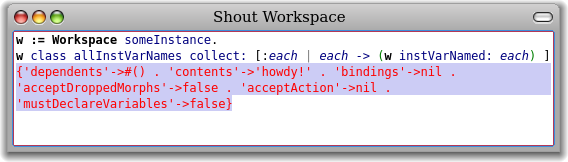
\includegraphics[width=\linewidth]{allInstanceVariables}
	\caption{Displaying all instance variables of a \ct!SystemWindow!.\label{fig:allInstanceVariables}}
\end{figure}

\figref{allInstanceVariables} shows how to display in a \ct!Transcript! the contents of the instance variables of an arbitrary instance (\ct!someInstance!) of class \ct!SystemWindow!.
The method \ct!allInstVarNames! returns all the names of the instance variables of a given class.

In the same spirit, it is possible to gather instances that have specific properties.
For instance, to get all instances of class \ct!Browser! whose instance variable \ct!systemOrganizer! is not \ct!nil!, try this expression:
\begin{code}{}
Browser allInstances select: [:c | (c instVarNamed: 'systemOrganizer') notNil]
\end{code}

%-----------------------------------------------------------------
\subsection{Iterating over instance variables}

Let us consider the message \ct!instanceVariableValues!, which returns a collection of all values of instance variables defined by this class, excluding the inherited instance variables.
For instance:
\begin{code}{@TEST}
(1@2) instanceVariableValues --> an OrderedCollection(1 2)
\end{code}

The method is implemented in \ct{Object} as follows:
\needlines{9}
\begin{code}{}
Object>>>instanceVariableValues
	"Answer a collection whose elements are the values of those instance variables of the receiver which were added by the receiver's class."	
	| c |
	c := OrderedCollection new.
	self class superclass instSize + 1
		to: self class instSize
		do: [ :i | c add: (self instVarAt: i)].
	^ c
\end{code}

% This example shows how useful it is to be able to access instance variables via their position \alex{maybe?: this example shows how index-based variable access is useful}
This method iterates over the indexes of instance variables that the class defines, starting just after the last index used by the superclasses.
(The method \ct!instSize! returns the number of all named instance variables that a class defines.)

%-----------------------------------------------------------------
\subsection{Querying classes and interfaces}

The development tools in \squeak (code browser, debugger, inspector...) all use the reflective features we have seen so far.

Here are a few other messages that might be useful to build development tools:


\lct{isKindOf: \emph{aClass}} returns true if the receiver is instance of \lct{\emph{aClass}} or of one of its superclasses.

For instance:
\begin{code}{@TEST}
1.5 class                     --> Float
1.5 isKindOf: Number --> true
1.5 isKindOf: Integer   --> false
\end{code}


\lct{respondsTo: \emph{aSymbol}} returns true if the receiver has a method whose selector is \lct{\emph{aSymbol}}.

For instance:
\begin{code}{@TEST}
1.5 respondsTo: #floor      --> true    "since Number implements floor"
1.5 floor                            --> 1
Exception respondsTo: #, --> true    "exception classes can be grouped"
\end{code}

Please note that these features are especially useful for defining development tools, but are normally not appropriate for typical applications.
Asking an object for its class, or querying it to discover which messages it understands, are typical signs of design problems, since they violate the principle of encapsulation.
Development tools, however, are not normal applications, since their domain is that of software itself. As such these tools have a right to dig deep into the internal details of code.

%Once again, the reflective features of \squeak are only useful to define development tools, and it is risky to use them to develop applications.
%Indeed, using the type of an object to drive execution of a method or another often reveals a design problem.

%\st offers other introspection possibilities for methods or the execution stack, the process scheduler, the memory manager... but we can't detail everything here; try to read the code and experiment by yourselves.

There also exist mechanisms for introspecting on various parts of the run-time system, such as compiled methods, the execution stack, the process scheduler, the memory manager and so on. For now we will focus on navigating through objects and classes, and we will look more closely at the runtime system in an other chapter.
\on{to be planned ...}

% section under_the_hood_instances (end)

%:======================================
\section{Browsing code} % (fold)

In \st, classes are normal objects, and they provide interesting features to navigate over their instances.
Most of the messages we will look at now are implemented in \ct{Behavior}, so they are understood by all classes.

As we saw previously, you can obtain an instance of a given class by sending it the message \ct!#someInstance!.

\begin{code}{} % Cannot test this
ByteString someInstance --> 'collection'
\end{code}

You can also gather all the instances with \ct!#allInstances!, or the number of alive instances in memory with \ct!#instanceCount!.

\begin{code}{} % Cannot test this
ByteString allInstances     --> #('collection' 'position'  ...)
ByteString instanceCount --> 104565
\end{code}

These features can be very useful when debugging an application, because you can ask a class to enumerate those of its methods that have specific properties.
\begin{itemize}
\item \ct!whichSelectorsAccess:! returns the list of all selectors of methods that read the instance variable named as the argument
\item \ct!whichSelectorsStoreInto:! returns the selectors of methods that modify the value of an instance variable
\item \ct!whichSelectorsReferTo:! returns the selectors of methods that send a given message
\item \ct!crossReference! associates each message with the set of methods that send it.
\end{itemize}

%\ct!an IdentitySet(#rotateBy:about: #translateBy: #isInsideCircle:with:with: #sideOf: #nearestPointAlongLineFrom:to: #normalized #eightNeighbors #dist: #hash #rotateBy:centerAt: #theta #grid: #fourNeighbors #dotProduct: #scaleFrom:to: #normal #onLineFrom:to:within: #+ #degrees #interpolateTo:at:)!.

\begin{code}{} % TOO FRAGILE TO TEST
Point whichSelectorsAccess: 'x'    --> an IdentitySet(#'\\' #= #scaleBy: ...)
Point whichSelectorsStoreInto: 'x' --> an IdentitySet(#setX:setY: ...)
Point whichSelectorsReferTo: #+  --> an IdentitySet(#rotateBy:about: ...)
Point crossReference --> an Array(
		an Array('*' an IdentitySet(#rotateBy:about: ...))
		an Array('+' an IdentitySet(#rotateBy:about: ...))
		...)
\end{code}

The following messages take inheritance into account:
\begin{itemize}
\item \ct{whichClassIncludesSelector:} returns the superclass that implements the given message
\item \ct{unreferencedInstanceVariables} returns the list of instance variables that are neither used in the receiver class nor any of its subclasses
\end{itemize}

\begin{code}{@TEST}
Rectangle whichClassIncludesSelector: #inspect --> Object
Rectangle unreferencedInstanceVariables            --> #()
\end{code}

\ct{SystemNavigation} is a facade that supports various useful methods for querying and browsing the source code of the system.
\ct!SystemNavigation default! returns an instance you can use to navigate the system.
For example:

\begin{code}{@TEST}
SystemNavigation default allClassesImplementing: #ifTrue: --> {Boolean. True. False}
\end{code}

%\ct!SystemNavigation default allClassesImplementing: #+! returns all classes that implement the message \ct!#+!.
%	In this case we get \ct!an Array(Number Fraction Float Integer SmallInteger LargePositiveInteger ScaledDecimal DateAndTime Duration Timespan Player Color Collection WordArray FloatArray KedamaFloatArray String Interval AbstractSound MixedSound Point Voice Complex TraitDescription TraitComposition TraitTransformation TComposingDescription)!.
%	As you can see, it is possible to add integers, fractions, strings or intervals.

The following messages should also be self-explanatory:

\begin{code}{}
SystemNavigation default allSentMessages size          --> 24930
SystemNavigation default allUnsentMessages size      --> 6431
SystemNavigation default allUnimplementedCalls size --> 270
\end{code}

Note that messages implemented but not sent are not necessarily useless, since they may be sent implicitly (\eg, using \ct{perform:}).
Messages sent but not implemented, however, are more problematic, because the methods sending these messages will fail at runtime.
They may be a sign of unfinished implementation, obsolete APIs, or missing libraries.


\ct!SystemNavigation default allCallsOn: #Point! returns all messages sent explicitly to \ct!Point! as a receiver.



All these features are integrated in the programming environment of \squeak, in particular in the code browsers.
As shown in \secref{cha:env}, you can list all methods that have the same name (implementors) or all methods that send a message (senders).
This is quite handy: for instance, when you want to change the name of a method, to check that you didn't miss one message send that could invoke this method (\figref{implementors}). \damien{is "invoke a method" OK here?}

\begin{figure}[ht]\centering
	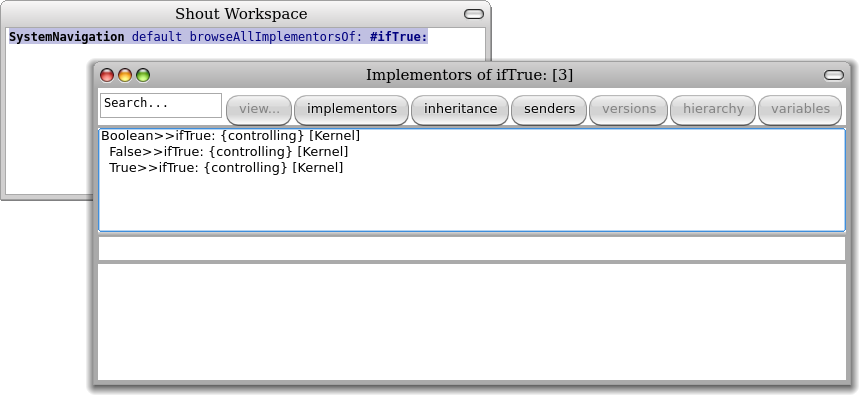
\includegraphics[width=.75\linewidth]{implementors}
	\caption{Displaying all classes that implement \ct!\#+!.\label{fig:implementors}}
\end{figure}

To see the internal structure of a class, you can inspect it like any object.
In \figref{CompiledMethod}, the inspector at the back shows the structure of class \ct!Point!.
You can see that the class stores its methods in a dictionary, indexing them by their selector.
The frontmost inspector shows the decompiled bytecode of \ct!Point!'s method \ct!#*!.

\begin{figure}[ht]\centering
	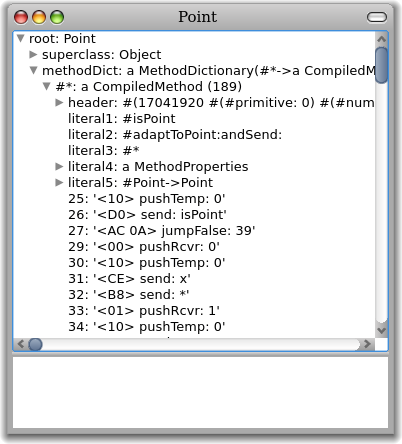
\includegraphics[width=.75\linewidth]{CompiledMethod}
	\caption{Inspecting class \ct!Point! and the bytecode of its \ct!\#*! method.\label{fig:CompiledMethod}}
	\on{re-do with white background!}
\end{figure}

\st is really a completely open and transparent system, where all the code is available for reading.
You can study the whole system as you wish, because there is no hidden code.
The primitive part of the system, \ie which is not written in \st, is reduced to its simplest expression.
Among \st dialects, \squeak has the peculiarity that even its virtual machine is written in \st, so it is possible to run and debug it inside a \squeak image!
Though this actually works, it is quite slow, and for actual use the virtual machine is translated to C and compiled to a native executable.

% section browsing_the_code (end)

%=================================================================
\section{Practical uses for introspection} % (fold)

%-----------------------------------------------------------------
\subsection{Code metrics}

Let's see how we can use \st's introspection features to quickly define code metrics.
A code metric is a measure of program code like depth in the inheritance hierarchy, the number of direct or indeirect subclasses, the number of methods or of instance variables in each class, or the number of locally defined methods or instance variables.
When discovering the code of a new application, you can evaluate a metric to get a rough idea of what the code looks like.
\scrref{metrics} computes a few code metrics for Morphic; these numbers can vary depending on the image you are using.
Results for class \ct!Morph!, which is the superclass of all graphical objects in \squeak, reveal that it is a huge class, and that it is at the root of a huge hierarchy. Maybe it needs some refactoring!

\begin{script}[metrics]{A few code metrics}
	inheritanceDepth := Morph allSuperclasses size. "2"
	methods := Morph allSelectors size. "1593"
	instVars := Morph allInstVarNames size. "6"
	addedMethods := Morph selectors size. "1165"
	addedInstVars := Morph instVarNames size. "6"
	directSubclasses := Morph subclasses size. "45"
	totalSubclasses := Morph allSubclasses size. "412"
\end{script}

One of the most interesting metrics in the domain of object-oriented languages is the number of methods that extend methods inherited from the superclass.
This informs us about the relation between the class and its superclasses.

Here is a script that identifies methods in class \ct!Browser! that call the method they redefine, like this:
\begin{code}{}
Browser >>> xx
	"..."
	super xx
\end{code}

\begin{script}[browsersendstosuper]{Methods of \ct!Browser! redefining via \ct!super!}
Browser selectors select: [ :eachSelector |
	| method |
	method := Browser compiledMethodAt: eachSelector.
	method sendsToSuper ]
\end{script}

In this code, we ask to class \ct!Browser! all messages it understands (\ct!selectors!) then select those whose associated method makes a call to the superclass.
This returns a collection of methods, containing for instance \ct!#veryDeepInner!.
You can see that the \st bytecode itself is viewed as an object that we can query for information.
We could even imagine methods that transform this bytecode.

%-----------------------------------------------------------------
\subsection{Detecting possible errors}

Sending a message to \ct!super! is a bad idea when that message is different from the one the current method implements.
This practice often causes bugs when adding subclasses, so good developers avoids that pattern of code.
It's easy to automatically identify occurences of this pattern: we simply have to find methods that make super-sends with a different selector than their own.

\begin{script}[findSuperSends]{Identifying bad super-sends}
Collection selectors select: [ :eachSelector |
	| method |
	method := Collection compiledMethodAt: eachSelector.
	method sendsToSuper and: [(method messages includes: eachSelector) not]]
\end{script}

Note that this script doesn't find everything we want... it doesn't detect methods containing loops or recursion like the following:
\begin{code}{}
xxx
	super yyy. "send something else than xxx to super"
	self zzz
\end{code}

When executing \scrref{findSuperSends} on class \ct!Collection!, you should obtain method \ct!printNameOn:! which does send \ct!printOn:! to \super:
\begin{method}[printNameOn]{A method that sends a different message to super}
Collection>>>printNameOn: aStream
	super printOn: aStream
\end{method}

In fact this method is used by \ct!printOn:! (\mthref{oldPrintOn}), which could be refactored as in \mthref{newPrintOn}.

\begin{method}[oldPrintOn]{The sender of \lct{\#printNameOn:}}
Collection>>>printOn: aStream
	"Append a sequence of characters that identify the receiver to aStream."
	self printNameOn: aStream.
	self printElementsOn: aStream
\end{method}

\begin{method}[newPrintOn]{New version of \mthref{oldPrintOn}, after inlining the \lct{\#printNameOn:} super-send}
Collection>>>printOn: aStream
	"Append a sequence of characters that identify the receiver to aStream."
	super printOn: aStream.
	self printElementsOn: aStream
\end{method}

Now \ct!#printNameOn:! (\mthref{printNameOn}) is not needed anymore. Well, in this case... is it used in other classes? Let's ask \squeak:
\begin{example}[sendersofprintnameon]{Asking for the senders of \lct{\#printNameOn:}}{}
SystemNavigator default allCallsOn: #printNameOn:
--> an OrderedCollection(A MethodReference RunArray >> printOn: aMethodReference Bitmap >> printOn: aMethodReference Text >> printOn: aMethodReference CompiledMethod >> printOn:)
\end{example}

So we should also refactor classes \clsind{RunArray}, \clsind{BitMap}, \clsind{Text}, and \clsind{CompiledMethod} that are sending message \ct!#printNameOn:!.

%-----------------------------------------------------------------
\subsection{Intelligent breakpoints}

In the 3.8 version of \squeak introduced a new kind of breakpoints.
Those are quite useful and are implemented by the \ct!Object>>>haltIf:! method.
This breakpoint only halts program execution if the method it's placed in was called by the one whose name was passed as an argument.
This is very useful to halt a method only during the execution of a test and not every time it is called.
For instance, the expression \ct!self haltIf: #testFoo! will only halt execution of its containing method if this method was called, directly or indirectly, from \ct!testFoo!.
The definition of \ct!haltIf:! is quite simple and fits in five lines; it uses the pseudo-variable \ct!thisContext!, which refers to the execution stack, represented as an object (\ct!thisContext! is one of the six keywords in Smalltalk, with \self, \super, \nil, \ct!true!, and \ct!false!).

\begin{method}[objecthaltif]{Implementation of a conditional breakpoint}
Object>>>haltIf: condition
	"This is the typical message to use for inserting breakpoints during debugging. Param can be a block or expression, halt if true.
	If the condition is a selector, we look up in the callchain. Halt if any method's selector equals selector."
	| cntxt |
	cntxt := thisContext.
	[cntxt sender isNil] whileFalse: [
		cntxt := cntxt sender.
		(cntxt selector = condition) ifTrue: [Halt signal]].
	^self.
\end{method}

Starting from \ct!thisContext!, \ct!haltIf:! goes up through the execution stack, checking if the name of the calling method is the same as the one passed as parameter.
If this is the case, then it raises an exception which, by default, summons the debugger.
This example shows the power of Smalltalk, which allows to define powerful features and tools from within the language itself.

The pseudo-variable \ct!thisContext! is especially used in the \squeak debugger.
It contains an instance of the \clsind{MethodContext} class.
This instance contains information about the method that is being executed, the stack pointer (\ct!stackpc!), and the program pointer (\ct!pc!).

In the following example, we halted \squeak's evaluation loop by pressing \short{.} and inspecting the current context.

\begin{figure}[ht]\centering
	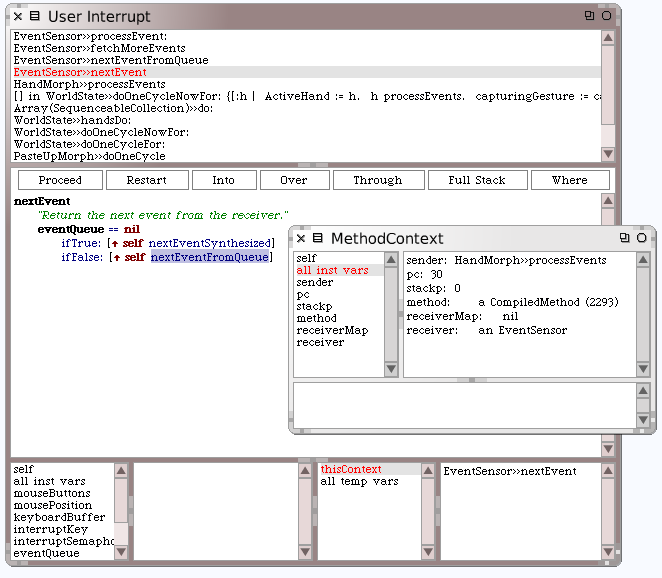
\includegraphics[width=\linewidth]{MethodContext}
	\caption{Inspecting the execution context of the evaluation loop in \squeak.\label{fig:MethodContext}}
\end{figure}

Via \ct!thisContext!, the Seaside web framework also accesses the execution stack, but it modifies it on the fly to easily implement reusable components over HTTP.

% section practical_uses_for_introspection (end)


%:======================================
\section{Object and Class meta-operations}

\on{uml}

\on{Object perform:}

%:======================================
\section{Controlling messages}

\on{
- override doesNotUnderstand\\
--- trap msgs sent to an object (with Proxy and with msgNotUnderstood)\\
- anonymous classes (see slides)\\
- method wrappers
}

\on{Object primitiveChangeClassTo: become: and becomeForward: (see slides with minimal object example)}

\on{- thisContext -- used in haltIf:}

%:======================================
\section{Methods as first class entities}

Compared to other reflective programming languages, \squeak is a Smalltalk implementation that brings reflection a step further. Whereas it handles \emph{methods as first class entities} that can be modified and replaced on the fly, it also allows for \emph{method execution reification}, exposing dynamic information related to method execution as objects.


\on{
- Methods as Objects; compiled methods; wrappers; spy\\
--- method dictionaries and compiled methods -- compiling, invoking \& removing methods\\
--- method wrappers: coverage; memoization\\
--- coverage checking of a class w. method wrappers\\
--- automatic memoization with method wrappers\\
}

\on{;""Q How do I check which methods of my package are not covered by tests?""
;""A"" Load the *http://www.squeaksource.com/ObjectsAsMethodsWrap.html* SqueakSource project and run:}

\begin{code}{}
category := 'SCGPier'.
w := (ObjectAsOneTimeMethodWrapper installOnClassCategory: category).

tr := TestRunner new.
ToolBuilder open: tr.
[tr
	categoryAt: (tr categoryList indexOf: 'SCGPier') put: true;
	selectAllClasses;
	runAll.]
ensure: [[w do: [:each| each uninstall ]] valueUnpreemptively].

((w select: [:each | each executed not ])
	collect: [:each | each wrappedClass name, '>>', each selector name ]) explore.
\end{code}


%-------------------------------------------------------------------------
\subsection{Reification of Methods} 

In Squeak, both classes and methods are represented by first class objects that can be accessed and even changed at runtime. 

\emph{Compiled methods} are objects in Squeak that describe the executable part of methods. A compiled method contains a pointer to the source code and the code executed by the virtual machine, the bytecode.

Compiled methods are stored in a method dictionary, in which keys are method names and values corresponding compiled methods. A method dictionary may be accessed from a given class by sending the message \ct{methodDict} to this class. For instance, the expression \ct{ExampleClass methodDict} returns the dictionary of methods for the class \ct{ExampleClass}.

Method dictionaries provide an interface for adding or replacing methods. When a new method is added from a development tool, such as the system browser, in essence, the system adds a new entry in the method dictionary of the class in which the method has been compiled for:

\begin{code}{}
ExampleClass methodDict at: #myMethod put: aCompiledMethod
\end{code}

A compiled method (\ct{aCompiledMethod}) is added to the method dictionary of the class \ct{ExampleClass} under the name \ct{myMethod}. The effect is the addition of a new method.

Having compiled methods as plain objects is a characteristic shared by most Smalltalk implementations. As we shall see in the coming section, one particularity of Squeak is to not restrict values contained in a method dictionary to be instances of \ct{CompiledMethod}.

%-------------------------------------------------------------------------
\subsection{Reification of method execution}

When a message named \emph{meth} is sent to an object, the class of receiver looks up the method to use to handle the message. If this class does have a method, it asks its superclass, and so on, up the inheritance chain. Once the method named \emph{meth} found in one of the superclass (\ie its method dictionary contains an entry for \emph{meth}), then the corresponding value associated with \emph{meth} is fetched from the method dictionary by the virtual machine (VM).

Once fetch, this method gets interpreted by the VM. At that stage, one of two cases happens: either this method is a \emph{compiled method} as we have seen previously, or it is a plain object that is not a compiled method. If this value is a compiled method (an instance of the class \ct{CompiledMethod}), then the VM directly interprets the bytecode. If this value is \emph{not} a compiled method, then the VM performs a \emph{reification of the method execution}.

This method execution reification is performed by the VM when sending the message \ct{run: methodName with: listOfArguments in: receiver} to this object method. In such a case, \ct{methodName} contains the name of the method currently invoked, \ct{listOfArguments} contains the list of arguments provided, and \ct{receiver} a reference to the receiver to the message.

For instance, let assume two classes, \ct{C} and \ct{Wrapper}:

\begin{code}{}
Object subclass: #C
	instanceVariableNames: ''
	classVariableNames: ''
	poolDictionaries: ''
	category: 'Example'.
 
Object subclass: #Wrapper
	instanceVariableNames: ''
	classVariableNames: ''
	poolDictionaries: ''
	category: 'Example'.
\end{code}

The class \ct{Wrapper} contains a method named \ct{run:with:in:} that takes three arguments, a name (\ct{methodName}), an array of objects (\ct{listOfArguments}), and an object reference (\ct{receiver}):

\begin{code}{}
Wrapper>>>run: methodName with: listOfArguments in: receiver
	"We first display some info on the standard output stream"
	Transcript show: 'Method ', methodName,
		' arguments: ', listOfArguments printString,
		' receiver: ', receiver printString.

	"Then we return the first element of the provided list"
	^ listOfArguments first
\end{code}

Prior to returning the first elements of \ct{listOfArguments}, some information is written to the standard output stream.

%The set of methods defined by a class is contained in a method dictionary, which can be accessed by sending the message \ct{methodDict} to a class. 
As we have seen in the previous section, a method \ct{foo:} is added to the class \ct{C} by altering its method dictionary:

\begin{code}{}
"We create an instance of Wrapper"
w := Wrapper new.

"We create an instance of C"
c := C new.

"We add a new method named foo: to C"
C methodDict at: #foo: put: w.
\end{code}

The last line above adds an entry named \ct{foo:} to the method dictionary of \ct{C}. Instances of \ct{C} therefore understand messages named \ct{foo:}. Because of the method execution reification mechanism, evaluating \ct{c foo: 10} is in fact evaluated by the VM as:

\begin{code}{}
w run: #foo: with: #(10) in: c
\end{code}

The result is \ct{10}, and displays the following on the standard output stream:

\begin{code}{}
Method foo: arguments: #(10) receiver: a C
\end{code}

Reification of method execution is an expressive mechanism that enables a whole range of dynamic meta operations. As an example, 

%-----------------------------------------------------------------
\subsection{Example with Spy}

As an illustration of section given above, this section presents \emph{Spy}, a small application that infers relationship between classes at runtime. Spy is available on SqueakSource\footnote{\url{http://www.squeaksource.com/Spy}}. 

A spy is installed on any class, with an \ct{installOn:} method and is removed by sending \ct{removeSpy} to a spied class. Spy is used as follows: 
\begin{itemize}
\item \ct{Spy installOn: aClass} -- installs a spy on a class \ct{aClass};
\item \ct{aClass stat} -- returns a textual description of the interaction of \ct{aClass};
\item \ct{aClass removeSpy} -- removes the spy from the class.
\end{itemize}

The idea is the following: installing spy will replace all compiled method of the class with instance of the class \ct{Spy}. Each instance of these instance knows the compiled method it has replaced. At runtime, each spy evaluates its compiled methods and uses introspection to extract dynamic information.

\ct{Spy} is a subclass of \ct{Object}
\begin{code}{}
Object subclass: #Spy
	instanceVariableNames: 'originalMethod nbOfcalls callingClasses selector'
	classVariableNames: ''
	poolDictionaries: ''
	category: 'Spy'
\end{code}

Few accessors and an initialization are necessary:
\begin{code}{}
Spy>>>callingClasses
	^ callingClasses ifNil: [callingClasses := OrderedCollection new]

Spy>>>originalMethod
	^ originalMethod

Spy>>>originalMethod: aCompiledMethod
	originalMethod := aCompiledMethod 

Spy>>>initialize
	super initialize.
	nbOfcalls := 0.
\end{code}

The variable \ct{callingClasses} will contains the classes that the spied class interact with. The compiled method the spy will replace is referenced by \ct{originalMethod}.

The main method is \ct{run:with:in:}:
\begin{code}{}
Spy>>>run: methodName with: listOfArguments in: receiver
	| callingClass |
	callingClass := thisContext sender receiver class.
	(self callingClasses includes: callingClass)
		ifFalse: [self callingClasses add: callingClass].
	nbOfcalls := nbOfcalls + 1.
		
	^ originalMethod valueWithReceiver: receiver arguments: listOfArguments 
\end{code}

The pseudo variable \ct{topContext} represents the top frame of the run-time stack. The frame below the top one is the result of \ct{thisContext sender}. The class of the receiver of this frame is obtained by sending the message \ct{receiver} and \ct{class}. This class is then inserted into \ct{callingClasses}. The compiled method is then evaluated on the receiver of the original message (and not the spy!) with the same arguments.

The Squeak interpreter may have to remove all references to this method form its method look cache. The following has to be defined as well:

\begin{code}{}
Spy>>>flushCache
	<primitive: 116>
\end{code}

Note that each object intended to replace a compiled method in a method dictionary has to understand this method.

Each spy is able to generate a little summary:

\begin{code}{}
Spy>>>summary
	^ selector printString, ' has been called: ', nbOfcalls asString, ' by ', self callingClasses asString
\end{code}

The \ct{installOn:} method will replace each compiled method with an instance of \ct{Spy}. Note that this method has to be defined on the class side:

\begin{code}{}
Spy class>>>installOn: aClass
	| dict cm |
	dict := aClass methodDictionary.
	dict keys do:
		[:k|
			cm := dict at: k.
			cm isCompiledMethod 
			 	ifTrue: [dict at: k put: (self new originalMethod: cm; selector: k; yourself)]]
			
\end{code}

The \ct{Spy} class is fully defined. The \ct{Behavior} class needs to be extended with few methods:

\begin{code}{}
Behavior>>>removeSpy
	| v |
	self methodDictionary keys do:
		[:k|
			v := self methodDict at: k. 
			(v class == Spy)
					ifTrue: [self methodDict at: k put: v originalMethod]]

Behavior>>>stat
	| ans |
	ans := ''.
	self methodDict values do: 
		[:spy|
				(spy isKindOf: Spy)
					ifTrue: [ans := ans, spy summary, String cr]].
	^ ans
\end{code}

The Spy application is now fully defined. As an example of usage, a spy may be installed on the class \ct{Stream} with \ct{Spy installOn: Stream}. Then print the result of \ct{Spy stat}. You should have something that looks like:

\begin{code}{}
 '#next:put: has been called: 0 by an OrderedCollection()
...
#basicNextPut: has been called: 71 by an OrderedCollection(Latin1TextConverter)
...
#nextPutAll: has been called: 27 by an OrderedCollection(WriteStream LimitedWriteStream)
...
'
\end{code}

\ct{Stream} may be freed from its spy with \ct{Stream removeSpy}.


%:======================================
\section{Chapter summary}

It is natural to use the reflective features in Smalltalk.
Indeed, the whole development environment and its code browsers are built using the introspective interfaces of objects and classes.
We want to stress that it is really interesting to be able to access and modify the objects that represent the program; it makes it unneccessary to devise alternative representations such as abstract syntax trees to build development tools (like Eclipse).
To fix Java~1.0's lack in this respect, Java~1.2 added the ``reflextive'' API ---which is actually only introspective.
Moreover, if the classes and other objects underlying the program execution offer introspective interfaces, then all program representations stay synchronized with the code at all times.
It is thus not needed to keep these representations up-to-date anymore.



%=================================================================
\ifx\wholebook\relax\else\end{document}\fi
%=================================================================

%-----------------------------------------------------------------
\subsection{XXX}
